\documentclass[12pt, a4paper]{article}

\usepackage[utf8]{inputenc}
\usepackage[T1]{fontenc}
\usepackage[left=2.5cm, right=2.5cm, top=3cm, bottom=3cm]{geometry}
\usepackage{graphicx}
\usepackage{tikz}
\usepackage{xcolor}
\usepackage{titlesec}
\usepackage{listings}
\usepackage{hyperref}
\usepackage{tcolorbox}
\tcbuselibrary{skins, breakable}
\usepackage{lmodern}
\usepackage{amsmath, amssymb}
\usepackage{enumitem}
\usepackage{array}

\renewcommand{\contentsname}{Índice}

\definecolor{RetroForgeDark}{HTML}{1E1E24}
\definecolor{RetroForgeOrange}{HTML}{FF6B35}
\definecolor{RetroForgeRed}{HTML}{E84855}
\definecolor{RetroForgePurple}{HTML}{7A28CB}
\definecolor{RetroForgeBlue}{HTML}{00A8E8}
\definecolor{RetroForgeBg}{HTML}{1E1E24}

\pagecolor{RetroForgeBg}
\AtBeginDocument{\color{white}}

\hypersetup{
    colorlinks=true,
    linkcolor=RetroForgeOrange,
    urlcolor=RetroForgeBlue,
    pdftitle={RetroForge - Guia de Estudos e Arquitetura}
}

\titleformat{\section}
  {\normalfont\Large\bfseries\color{RetroForgePurple}}
  {\thesection}{1em}{}
  [{\color{RetroForgePurple}\titlerule[0.8pt]}]

\titleformat{\subsection}
  {\normalfont\large\bfseries\color{RetroForgeRed}}
  {\thesubsection}{1em}{}

\titleformat{\subsubsection}
  {\normalfont\normalsize\bfseries\color{RetroForgeBlue}}
  {\thesubsubsection}{1em}{}

\tcbuselibrary{skins, breakable, most, listings}

\lstdefinestyle{RetroForgeCode}{
    basicstyle=\ttfamily\small\color{white},
    keywordstyle=\color{RetroForgeOrange}\bfseries,
    commentstyle=\color{gray},
    stringstyle=\color{RetroForgeBlue},
    breaklines=true,
    showstringspaces=false,
    tabsize=4,
    language=C++,
    numbers=left,
    numberstyle=\tiny\color{gray},
    numbersep=8pt,
}

\newtcolorbox{CaixaInfo}[1][]{
    enhanced,
    breakable,
    colback=RetroForgeDark!90!RetroForgeBlue,
    colframe=RetroForgeBlue,
    coltitle=white,
    coltext=white,
    title={\textbf{Dica / Info}},
    attach boxed title to top left={xshift=5mm, yshift=-3mm},
    boxed title style={size=small, colback=RetroForgeBlue, colframe=RetroForgeBlue, rounded corners},
    drop fuzzy shadow,
    #1
}

\newtcolorbox{CaixaAlerta}[1][]{
    enhanced,
    breakable,
    colback=RetroForgeDark!90!RetroForgeOrange,
    colframe=RetroForgeOrange,
    coltitle=white,
    coltext=white,
    title={\textbf{Atenção / Alerta}},
    attach boxed title to top left={xshift=5mm, yshift=-3mm},
    boxed title style={size=small, colback=RetroForgeOrange, colframe=RetroForgeOrange, rounded corners},
    drop fuzzy shadow,
    #1
}

\newtcblisting{CaixaCodigo}{
    enhanced,
    breakable,
    colback=RetroForgeDark!95!white,
    colframe=RetroForgeDark,
    coltext=white!90,
    title={\textbf{Fragmento de Código}},
    attach boxed title to top left={xshift=5mm, yshift=-3mm},
    boxed title style={size=small, colback=RetroForgeDark, colframe=RetroForgeDark, rounded corners},
    drop fuzzy shadow,
    listing only,
    listing options={style=RetroForgeCode},
}

\lstdefinestyle{RetroForgeTree}{
    basicstyle=\ttfamily\small\color{white},
    breaklines=false,
    showstringspaces=false,
    tabsize=2,
}

\newtcblisting{CaixaArvore}{
    enhanced,
    breakable,
    colback=RetroForgeDark!95!white,
    colframe=RetroForgePurple,
    coltext=white!90,
    title={\textbf{Estrutura de Pastas}},
    attach boxed title to top left={xshift=5mm, yshift=-3mm},
    boxed title style={size=small, colback=RetroForgePurple, colframe=RetroForgePurple, rounded corners},
    drop fuzzy shadow,
    listing only,
    listing options={style=RetroForgeTree},
}

\newtcolorbox{CaixaDesafio}[1][]{
    enhanced,
    breakable,
    colback=RetroForgeDark!90!RetroForgePurple,
    colframe=RetroForgePurple,
    coltitle=white,
    coltext=white,
    title={\textbf{Desafio Prático}},
    attach boxed title to top left={xshift=5mm, yshift=-3mm},
    boxed title style={size=small, colback=RetroForgePurple, colframe=RetroForgePurple, rounded corners},
    drop fuzzy shadow,
    #1
}

\newtcolorbox{CaixaResumo}[1][]{
    enhanced,
    breakable,
    colback=RetroForgeDark!90!RetroForgeRed,
    colframe=RetroForgeRed,
    coltitle=white,
    coltext=white,
    title={\textbf{Resumo do Módulo}},
    attach boxed title to top left={xshift=5mm, yshift=-3mm},
    boxed title style={size=small, colback=RetroForgeRed, colframe=RetroForgeRed, rounded corners},
    drop fuzzy shadow,
    #1
}

\begin{document}

\begin{titlepage}
    \begin{tikzpicture}[remember picture, overlay]
        \fill[RetroForgeDark] (current page.south west) rectangle (current page.north east);
 
        \draw[RetroForgePurple, thick] (current page.south west) grid[step=1cm] (current page.north east);
        \fill[RetroForgeDark, opacity=0.8] (current page.south west) rectangle (current page.north east);

        \fill[RetroForgeOrange] (current page.north) circle (3cm);
        \fill[RetroForgeRed, opacity=0.7] (current page.north) circle (2.5cm);
 
        \node[text=white, font=\Huge\bfseries\sffamily, align=center] at (current page.center) {
            \scalebox{2.5}{RETRO}\\[0.2cm]
            \scalebox{2.5}{\color{RetroForgeOrange}FORGE}
        };
 
        \node[text=white, font=\large, align=center, yshift=-3cm] at (current page.center) {
            GUIA DEFINITIVO DE ARQUITETURA\\
            E ESTUDOS EM C++ MODERNO
        };
 
        \node[text=RetroForgeBlue, font=\normalsize, align=center, yshift=-10cm] at (current page.center) {
            DOCUMENTAÇÃO OFICIAL\\
            v1.0.0
        };
    \end{tikzpicture}
\end{titlepage}

\newpage
\tableofcontents
\newpage

\section{Módulo 0: A Fundação em C++ (O Core de Alta Performance)}

O RetroForge não é um script utilitário qualquer: é uma ferramenta que vai varrer discos rígidos inteiros, abrir arquivos de múltiplos gigabytes, disparar processos externos em paralelo e, ainda assim, se comportar de forma previsível e segura. Nada disso é possível se a fundação em C++ estiver mal construída. Antes de escrever uma única linha do Motor de Identificação ou do Thread Pool, precisamos dominar quatro pilares que sustentam absolutamente tudo o que vem depois:

\begin{enumerate}[label=\textbf{\arabic*.}]
    \item \textbf{Orientação a Objetos e Princípios SOLID} -- como vamos organizar o código em classes coesas, desacopladas e extensíveis.
    \item \textbf{Arquitetura de Pastas} -- onde cada classe mora e por quê.
    \item \textbf{Manipulação Binária de Arquivos} -- ler ISOs, BINs e CUEs sem jogar 4 GB inteiros na RAM.
    \item \textbf{Gerenciamento de Memória via Smart Pointers} -- eliminar vazamentos enquanto o programa varre um HD inteiro e dispara subprocessos.
    \item \textbf{Estruturas de Dados Eficientes e Polimorfismo} -- escolher a coleção certa e a abstração certa para caminhos, metadados, filas e roteamento de consoles.
\end{enumerate}

\begin{CaixaInfo}
Este módulo é deliberadamente mais denso em teoria do que os módulos seguintes. É aqui que erros de arquitetura --- se cometidos --- se propagam para o resto do projeto inteiro. A partir daqui, \textbf{todo módulo deste livro vai introduzir classes reais}, explicando para cada uma: (1) por que ela existe, (2) como ela se comunica com as demais, e (3) em qual pasta do projeto ela mora. Vale a pena ler este módulo duas vezes -- ele define o vocabulário e as convenções que os módulos 1 a 14 vão assumir como já conhecidas.
\end{CaixaInfo}

\subsection{Por que C++17/20 e não C, Rust ou uma linguagem gerenciada?}

Antes de mergulhar em código, é importante justificar a escolha tecnológica que baliza todo o RetroForge.

\begin{itemize}
    \item \textbf{Zero-cost abstractions:} em C++ moderno, escrever código orientado a objetos e seguro (RAII, smart pointers, classes com interfaces bem definidas) não impõe overhead de performance em tempo de execução comparado ao C puro escrito ``na unha''. Pagamos o custo apenas em tempo de compilação -- nunca em tempo de execução.
    \item \textbf{Controle de baixo nível quando necessário:} precisamos de acesso a \texttt{mmap}/\texttt{MapViewOfFile}, chamadas POSIX de processos e leitura de bytes crus de um disco. Linguagens totalmente gerenciadas (Java, C\#, Python puro) escondem esse nível de controle ou o tornam custoso.
    \item \textbf{Ecossistema de bibliotecas de compressão:} \texttt{chdman}, \texttt{maxcso} e \texttt{dolphin-tool} são, em sua maioria, projetos em C/C++. Integrar via subprocesso ou até estaticamente é mais natural nesse ecossistema.
    \item \textbf{Portabilidade binária:} com CMake e compilação estática, entregamos um executável único para Windows e Linux, sem exigir runtime como o .NET ou uma JVM instalada na máquina do usuário final.
\end{itemize}

\begin{CaixaAlerta}
C++ moderno (17/20) não é ``C com classes''. Se você escrever RetroForge usando \texttt{new}/\texttt{delete} manuais, \texttt{char*} crus e \texttt{system()} para tudo, você reintroduz exatamente os bugs de memória e segurança que estamos tentando evitar. A regra de ouro deste projeto é: \textbf{se você está gerenciando um recurso manualmente, provavelmente existe uma abstração da STL ou uma classe do próprio RetroForge que faz isso por você, de forma segura e sem custo extra.}
\end{CaixaAlerta}

\subsection{Orientação a Objetos e os Princípios SOLID no RetroForge}

O RetroForge não vai ser escrito como uma sequência de funções soltas em um único arquivo \texttt{main.cpp}. Cada responsabilidade do sistema -- ler bytes de um arquivo, identificar um console, gerenciar um processo externo, representar o estado de uma conversão -- vira uma \textbf{classe}, com um contrato (interface) claro e uma única razão para existir. Isso não é purismo acadêmico: é o que permite que a comunidade (Módulo 14) adicione suporte a um novo console \textit{sem tocar} no código que já funciona, e é o que permite testar (Módulo 12) cada peça isoladamente, sem precisar rodar o programa inteiro com um jogo de 4 GB.

Vamos usar os cinco princípios SOLID como bússola ao longo de todo o livro. Aqui está o que cada um significa, especificamente, dentro do RetroForge:

\begin{center}
\begin{tabular}{|>{\ttfamily}c|p{2.1cm}|p{7.3cm}|}
\hline
\textbf{Sigla} & \textbf{Princípio} & \textbf{O que significa no RetroForge} \\
\hline
S & Responsabilidade Única & Uma classe como \texttt{BinaryFileReader} só sabe ler bytes de um arquivo. Ela não sabe identificar consoles, não sabe comprimir, não sabe desenhar barra de progresso. \\
\hline
O & Aberto/Fechado & Para suportar um novo console (ex: PS3), criamos uma \textbf{nova} classe detectora. Não abrimos e editamos a classe \texttt{ConsoleIdentifier} que já está testada e funcionando. \\
\hline
L & Substituição de Liskov & Qualquer detector de console (\texttt{GameCubeDetector}, \texttt{Ps1Detector}, etc.) pode substituir outro dentro de \texttt{ConsoleIdentifier} sem quebrar o comportamento esperado do sistema. \\
\hline
I & Segregação de Interface & A interface \texttt{IConsoleDetector} tem só dois métodos. Não existe uma interface gigante ``\texttt{IEverything}'' que obriga uma classe a implementar coisas que ela não usa. \\
\hline
D & Inversão de Dependência & \texttt{ConsoleIdentifier} (regra de negócio de alto nível) depende da \textbf{abstração} \texttt{IConsoleDetector}, nunca de uma classe concreta como \texttt{GameCubeDetector} diretamente. \\
\hline
\end{tabular}
\end{center}

\begin{CaixaInfo}
Nem todo princípio SOLID se aplica com a mesma força em toda classe. Uma classe de dados simples, como veremos com \texttt{ConversionJob}, é essencialmente sobre Responsabilidade Única e encapsulamento -- não faz sentido forçar uma interface polimórfica nela só para ``usar SOLID''. Aplicar SOLID onde \textit{faz sentido} é, em si, uma decisão de engenharia -- e vamos justificar cada escolha ao longo do livro.
\end{CaixaInfo}

\subsection{Arquitetura de Pastas do Projeto}

A documentação do RetroForge já estabelece a regra mais importante de arquitetura: separação estrita entre a \textbf{Regra de Negócio (Core)} e a \textbf{Camada de Apresentação (CLI/GUI)}. O repositório atual já reflete o início dessa separação, com as pastas \texttt{core/} e \texttt{cli/} orquestradas por um \texttt{CMakeLists.txt} raiz. A partir deste módulo, vamos formalizar e expandir essa estrutura -- ela é o ``mapa'' que usaremos em todos os módulos seguintes para saber onde cada nova classe deve morar.

\begin{CaixaArvore}
RetroForge/
|-- CMakeLists.txt              (raiz: orquestra os subprojetos)
|-- core/                       (Regra de Negocio -- NUNCA depende de UI)
|   |-- CMakeLists.txt
|   |-- include/
|   |   `-- retroforge/
|   |       |-- io/
|   |       |   |-- BinaryFileReader.hpp
|   |       |-- process/
|   |       |   |-- ExternalProcessHandle.hpp
|   |       |-- identification/
|   |       |   |-- IConsoleDetector.hpp
|   |       |   |-- ConsoleIdentifier.hpp
|   |       |   `-- detectors/
|   |       |       |-- GameCubeDetector.hpp
|   |       |       `-- Ps1Detector.hpp
|   |       `-- models/
|   |           |-- Console.hpp
|   |           `-- ConversionJob.hpp
|   `-- src/
|       |-- io/
|       |   |-- BinaryFileReader.cpp
|       |-- process/
|       |   |-- ExternalProcessHandle.cpp
|       `-- identification/
|           |-- ConsoleIdentifier.cpp
|           `-- detectors/
|               |-- GameCubeDetector.cpp
|               `-- Ps1Detector.cpp
|-- cli/                        (Apresentacao: terminal, usa CLI11)
|   |-- CMakeLists.txt
|   `-- main.cpp
|-- gui/                        (Apresentacao: Dear ImGui -- futuro, Modulo 11)
|-- external/                   (dependencias de terceiros: CLI11, etc.)
`-- tests/                      (Modulo 12: Catch2 ou GTest)
\end{CaixaArvore}

\subsubsection{Por que separar \texttt{include/} de \texttt{src/}?}

Esta é uma convenção profissional de projetos C++ de médio/grande porte, e vamos segui-la a partir deste módulo:

\begin{itemize}
    \item \textbf{\texttt{include/retroforge/...}} contém apenas os arquivos \texttt{.hpp} -- a \textbf{API pública} de cada classe: o que ela promete fazer, sem revelar como. É isso que o \texttt{cli/} (e futuramente o \texttt{gui/}) vai enxergar via \texttt{target\_include\_directories}.
    \item \textbf{\texttt{src/...}} contém os arquivos \texttt{.cpp} -- a \textbf{implementação} de fato. Detalhes internos (como exatamente lemos os bytes, como exatamente chamamos \texttt{popen}) ficam isolados aqui e podem mudar livremente sem que o \texttt{cli/} precise recompilar contra uma nova interface.
    \item O prefixo \texttt{retroforge/} dentro de \texttt{include/} evita colisão de nomes quando o projeto crescer e for usado como dependência por outro projeto (um \texttt{\#include <retroforge/io/BinaryFileReader.hpp>} é inequívoco).
\end{itemize}

\subsubsection{Por que subpastas como \texttt{io/}, \texttt{process/}, \texttt{identification/} e \texttt{models/}?}

Cada subpasta corresponde a uma \textbf{área de responsabilidade} do sistema, não a um tipo de dado ou a uma camada técnica genérica. Isso é intencional: quando a comunidade (Módulo 14) quiser adicionar suporte à Xbox, ela sabe, sem perguntar a ninguém, que a nova classe \texttt{XboxDetector} vai morar em \texttt{core/include/retroforge/identification/detectors/} e sua implementação em \texttt{core/src/identification/detectors/}. A pasta \texttt{detectors/} dentro de \texttt{identification/} existe justamente para acomodar o crescimento previsto pelo Princípio Aberto/Fechado: ela vai ganhar um arquivo novo a cada console suportado, sem que os arquivos existentes precisem ser tocados.

A pasta \texttt{models/} tem um papel um pouco diferente das demais: ela não representa uma \textit{operação} do sistema (ler bytes, identificar, gerenciar um processo), mas sim \textbf{vocabulário e estado de domínio} -- tipos simples que várias áreas do projeto precisam compartilhar. É por isso que, mais adiante nesta seção, o \texttt{enum class Console} vai morar sozinho em \texttt{models/Console.hpp}, em vez de ser declarado dentro de \texttt{ConversionJob.hpp} ou de \texttt{IConsoleDetector.hpp}: tanto \texttt{models/} quanto \texttt{identification/} precisam do mesmo vocabulário, e nenhuma das duas áreas deveria ser dona exclusiva dele.

\begin{CaixaAlerta}
Nunca coloque lógica de negócio (identificação de console, roteamento de compressão, regras de conversão) dentro de \texttt{cli/} ou \texttt{gui/}. Se amanhã a comunidade decidir criar uma GUI em Qt em vez de Dear ImGui, ela deve conseguir reaproveitar 100\% do código em \texttt{core/} sem reescrever nenhuma regra de negócio -- só a apresentação muda.
\end{CaixaAlerta}

\subsection{Manipulação Binária de Arquivos}

O Motor de Identificação (Módulo 2) precisa ler os primeiros bytes de arquivos que podem ter dezenas de gigabytes (uma ISO de PS2 dual-layer, por exemplo). Se abrirmos esse arquivo da forma errada, ou pior, se tentarmos carregá-lo inteiro na memória, o RetroForge vai travar a máquina do usuário. Tudo começa com \texttt{<fstream>} e o entendimento correto do \textbf{modo binário}.

\subsubsection{Texto vs. Binário: por que o \texttt{ios::binary} é inegociável}

Por padrão, fluxos de arquivo em C++ podem operar em ``modo texto''. Em sistemas como Windows, o modo texto realiza uma tradução automática de quebras de linha (\texttt{\textbackslash n} $\leftrightarrow$ \texttt{\textbackslash r\textbackslash n}) e pode interpretar certos bytes (como \texttt{0x1A}, EOF de DOS) como fim de arquivo prematuro. Uma ISO ou um BIN é uma sequência arbitrária de bytes -- não texto -- e qualquer tradução automática \textbf{corrompe silenciosamente os dados lidos}.

\begin{CaixaAlerta}
Este é exatamente o tipo de bug que motivou o RetroForge: ferramentas que ``operam às cegas''. Esquecer a flag \texttt{std::ios::binary} ao abrir um \texttt{.iso} no Windows pode fazer o programa interpretar erroneamente o byte \texttt{0x1A} como fim de arquivo, cortando a leitura e gerando um Magic Number incorreto -- o que classificaria o console errado antes mesmo de começarmos a conversão.
\end{CaixaAlerta}

\begin{CaixaCodigo}
#include <fstream>
#include <iostream>

int main() {
    // SEMPRE combine ios::in (leitura) com ios::binary
    std::ifstream arquivo("jogo.iso", std::ios::in | std::ios::binary);

    if (!arquivo.is_open()) {
        std::cerr << "Erro: nao foi possivel abrir o arquivo.\n";
        return 1;
    }

    std::cout << "Arquivo aberto em modo binario com seguranca.\n";
    return 0;
}
\end{CaixaCodigo}

\subsubsection{Flags de abertura essenciais}

A tabela a seguir resume as flags de \texttt{std::ios} mais relevantes para o RetroForge:

\begin{center}
\begin{tabular}{|>{\ttfamily}l|p{9cm}|}
\hline
\textbf{Flag} & \textbf{Uso no RetroForge} \\
\hline
ios::in & Abrir para leitura (padrão para \texttt{ifstream}). Usado ao ler magic numbers e ao gerar hash. \\
\hline
ios::out & Abrir para escrita. Usado ao gravar logs (\texttt{retroforge\_errors.txt}) e arquivos temporários. \\
\hline
ios::binary & \textbf{Obrigatório} para qualquer arquivo de ROM/ISO/BIN. Nunca abrir uma imagem de disco sem esta flag. \\
\hline
ios::ate & Posiciona o cursor no final do arquivo já na abertura -- útil para descobrir o tamanho do arquivo rapidamente com \texttt{tellg()}. \\
\hline
ios::app & Acrescenta ao final do arquivo sem sobrescrever. Ideal para o log concorrente do Módulo 9. \\
\hline
\end{tabular}
\end{center}

\subsubsection{Lendo apenas o necessário: \texttt{seekg}, \texttt{tellg} e leitura posicionada}

O Motor de Identificação não precisa ler o arquivo inteiro -- ele só precisa dos primeiros kilobytes (ou de um offset específico, como o \texttt{0xC2339F3D} do GameCube na posição \texttt{0x1C}). Para isso usamos \texttt{seekg} (posicionar o cursor de leitura) e \texttt{read} (ler um número exato de bytes para um buffer).

\begin{CaixaCodigo}
#include <fstream>
#include <array>
#include <cstdint>
#include <iostream>

// Le 4 bytes a partir de um offset especifico do arquivo,
// sem carregar o restante do arquivo na memoria.
uint32_t ler_magic_number(const std::string& caminho, std::streamoff offset) {
    std::ifstream arquivo(caminho, std::ios::in | std::ios::binary);
    if (!arquivo) {
        throw std::runtime_error("Nao foi possivel abrir: " + caminho);
    }

    // Posiciona o cursor de leitura no offset desejado
    arquivo.seekg(offset, std::ios::beg);

    std::array<char, 4> buffer{};
    arquivo.read(buffer.data(), buffer.size());

    if (arquivo.gcount() != 4) {
        throw std::runtime_error("Arquivo truncado ou menor que o esperado.");
    }

    // Monta o inteiro de 32 bits a partir dos 4 bytes lidos (big-endian aqui)
    uint32_t valor =
        (static_cast<uint8_t>(buffer[0]) << 24) |
        (static_cast<uint8_t>(buffer[1]) << 16) |
        (static_cast<uint8_t>(buffer[2]) << 8)  |
        (static_cast<uint8_t>(buffer[3]));

    return valor;
}

int main() {
    // Assinatura de GameCube esperada na posicao 0x1C
    constexpr uint32_t MAGIC_GAMECUBE = 0xC2339F3D;

    uint32_t assinatura = ler_magic_number("jogo.iso", 0x1C);

    if (assinatura == MAGIC_GAMECUBE) {
        std::cout << "Console identificado: Nintendo GameCube\n";
    } else {
        std::cout << "Assinatura desconhecida: 0x" << std::hex << assinatura << "\n";
    }

    return 0;
}
\end{CaixaCodigo}

\begin{CaixaInfo}
Note o uso de \texttt{std::array<char, 4>} em vez de um \texttt{char[4]} cru. \texttt{std::array} tem tamanho fixo conhecido em tempo de compilação, não decai para ponteiro tão facilmente quanto um array C, e se integra naturalmente com \texttt{.data()} e \texttt{.size()} -- ambos aceitos por \texttt{read()}.
\end{CaixaInfo}

\subsubsection{Lendo arquivos grandes em blocos (\textit{chunks})}

Quando o objetivo não é apenas ler um cabeçalho, mas processar o arquivo inteiro -- como no Scraper Online (Seção 3.6 da documentação), que precisa gerar uma hash \texttt{xxHash} do arquivo completo --, a estratégia correta é ler em blocos de tamanho fixo (por exemplo, 4 MB) em vez de alocar um buffer do tamanho do arquivo inteiro.

\begin{CaixaCodigo}
#include <fstream>
#include <vector>
#include <cstdint>
#include <iostream>

constexpr size_t TAMANHO_CHUNK = 4 * 1024 * 1024; // 4 MB

void processar_arquivo_em_chunks(const std::string& caminho) {
    std::ifstream arquivo(caminho, std::ios::in | std::ios::binary);
    if (!arquivo) {
        throw std::runtime_error("Falha ao abrir arquivo para hashing.");
    }

    // Um unico buffer reutilizado a cada iteracao: sem realocacoes constantes
    std::vector<char> buffer(TAMANHO_CHUNK);

    while (arquivo) {
        arquivo.read(buffer.data(), buffer.size());
        std::streamsize bytes_lidos = arquivo.gcount();

        if (bytes_lidos <= 0) {
            break;
        }

        // Aqui entraria a chamada real: xxh64_update(estado_hash, buffer.data(), bytes_lidos);
        std::cout << "Processado bloco de " << bytes_lidos << " bytes.\n";
    }
}
\end{CaixaCodigo}

\begin{CaixaAlerta}
Nunca faça algo como \texttt{std::vector<char> tudo(tamanho\_do\_arquivo)} seguido de um único \texttt{read()} gigante para arquivos de ROM. Uma ISO de PS2 pode ter 4,7 GB; multiplique isso pelo número de threads simultâneas do Thread Pool (Módulo 4) e você terá um consumo de RAM absurdo e picos de alocação que podem derrubar o processo por falta de memória.
\end{CaixaAlerta}

\subsubsection{Encapsulando tudo: a classe \texttt{BinaryFileReader}}

As duas funções livres acima (\texttt{ler\_magic\_number} e \texttt{processar\_arquivo\_em\_chunks}) são ótimas para \textbf{entender o mecanismo}, mas não é assim que o código vai viver dentro do RetroForge. Funções soltas que abrem o próprio \texttt{ifstream} a cada chamada não podem ser reutilizadas, testadas isoladamente (Módulo 12) ou substituídas por uma implementação diferente (por exemplo, uma baseada em \textit{memory mapping}, Módulo 10) sem alterar quem as chama.

Por isso, encapsulamos essa responsabilidade em uma classe.

\begin{itemize}
    \item \textbf{Por que ela existe:} \texttt{BinaryFileReader} tem uma única razão para mudar -- a forma como lemos bytes de um arquivo binário (Princípio da Responsabilidade Única). Ela não sabe o que é um console, um magic number específico ou uma hash; isso é problema de quem a usa.
    \item \textbf{Como se comunica com outras classes:} \texttt{BinaryFileReader} é uma dependência de baixo nível. No Módulo 2, a classe \texttt{ConsoleIdentifier} (que veremos adiante nesta mesma seção) vai receber uma referência a um \texttt{BinaryFileReader} já aberto e chamar \texttt{read\_at(...)} para obter o cabeçalho do arquivo. Ela não sabe (nem precisa saber) que existe um \texttt{ConsoleIdentifier} -- a dependência é de mão única.
    \item \textbf{Onde ela mora:} declaração em \texttt{core/include/retroforge/io/BinaryFileReader.hpp}; implementação em \texttt{core/src/io/BinaryFileReader.cpp}.
\end{itemize}

\begin{CaixaCodigo}
// Arquivo: core/include/retroforge/io/BinaryFileReader.hpp
#pragma once

#include <cstdint>
#include <fstream>
#include <string>
#include <vector>

namespace retroforge::io {

// Responsabilidade unica: abrir e ler bytes de arquivos binarios de forma
// segura (RAII, via std::ifstream como membro) e eficiente (leitura
// posicionada e em blocos). Esta classe NAO sabe nada sobre consoles,
// hashes ou conversao -- isso pertence a outras classes.
class BinaryFileReader {
public:
    explicit BinaryFileReader(const std::string& caminho);

    // Le 'quantidade' bytes a partir de um offset absoluto do arquivo.
    std::vector<uint8_t> read_at(std::streamoff offset, size_t quantidade);

    // Le o proximo bloco sequencial de ate 'tamanho_maximo' bytes.
    // Retorna um vetor vazio quando o arquivo tiver acabado.
    std::vector<uint8_t> read_next_chunk(size_t tamanho_maximo);

    bool eof() const;
    std::uintmax_t tamanho_total() const { return tamanho_total_; }

private:
    std::ifstream arquivo_;       // RAII: fechado automaticamente no destrutor
    std::uintmax_t tamanho_total_;
};

} // namespace retroforge::io
\end{CaixaCodigo}

\begin{CaixaCodigo}
// Arquivo: core/src/io/BinaryFileReader.cpp
#include "retroforge/io/BinaryFileReader.hpp"

#include <filesystem>
#include <stdexcept>

namespace retroforge::io {

BinaryFileReader::BinaryFileReader(const std::string& caminho)
    : arquivo_(caminho, std::ios::in | std::ios::binary)
    , tamanho_total_(0) {

    if (!arquivo_.is_open()) {
        throw std::runtime_error("Nao foi possivel abrir: " + caminho);
    }

    tamanho_total_ = std::filesystem::file_size(caminho);
}

std::vector<uint8_t> BinaryFileReader::read_at(std::streamoff offset, size_t quantidade) {
    arquivo_.clear();               // limpa eventuais flags de erro/EOF anteriores
    arquivo_.seekg(offset, std::ios::beg);

    std::vector<uint8_t> buffer(quantidade);
    arquivo_.read(reinterpret_cast<char*>(buffer.data()), static_cast<std::streamsize>(quantidade));

    // Se o arquivo for menor que o esperado, encolhemos o vetor para o
    // tamanho realmente lido em vez de devolver lixo de memoria.
    buffer.resize(static_cast<size_t>(arquivo_.gcount()));
    return buffer;
}

std::vector<uint8_t> BinaryFileReader::read_next_chunk(size_t tamanho_maximo) {
    std::vector<uint8_t> buffer(tamanho_maximo);
    arquivo_.read(reinterpret_cast<char*>(buffer.data()), static_cast<std::streamsize>(tamanho_maximo));
    buffer.resize(static_cast<size_t>(arquivo_.gcount()));
    return buffer;
}

bool BinaryFileReader::eof() const {
    return arquivo_.eof();
}

} // namespace retroforge::io
\end{CaixaCodigo}

\begin{CaixaInfo}
Note que o construtor lança uma exceção (\texttt{std::runtime\_error}) em vez de retornar um código de erro. Como o único recurso gerenciado é o \texttt{std::ifstream} (que já é RAII por si só), não precisamos de nenhum \texttt{try/catch} manual aqui para liberar recursos -- se a exceção se propagar, o destrutor de \texttt{arquivo\_} cuida de tudo sozinho. Essa é a essência de RAII combinada com Orientação a Objetos: o objeto garante seu próprio ciclo de vida.
\end{CaixaInfo}

\subsection{RAII e Gerenciamento de Memória (Smart Pointers)}

RAII (\textit{Resource Acquisition Is Initialization}) é o princípio mais importante de todo o C++ moderno e será citado repetidamente ao longo deste ``livro''. A ideia é simples: \textbf{a aquisição de um recurso (memória, arquivo, handle de processo, mutex) acontece no construtor de um objeto, e a liberação acontece automaticamente no destrutor.} Isso significa que, se o objeto sai de escopo -- seja por um \texttt{return} normal, seja por uma exceção lançada no meio do caminho --, o recurso é liberado sem que o programador precise lembrar de fazê-lo manualmente.

\begin{CaixaInfo}
\texttt{std::ifstream} e \texttt{std::ofstream} já são exemplos de RAII: o arquivo é fechado automaticamente quando o objeto sai de escopo, mesmo sem uma chamada explícita a \texttt{close()}. É exatamente por isso que a classe \texttt{BinaryFileReader} da seção anterior não precisa de destrutor customizado -- ela delega o RAII do arquivo para o \texttt{std::ifstream} que já possui como membro. Smart pointers estendem esse mesmo princípio para memória alocada dinamicamente e para recursos externos, como handles de processos, que \textbf{não} são RAII por padrão.
\end{CaixaInfo}

\subsubsection{\texttt{std::unique\_ptr}: posse exclusiva}

\texttt{std::unique\_ptr} representa posse exclusiva de um recurso: só pode existir um \texttt{unique\_ptr} apontando para aquele recurso em um dado momento (ele não pode ser copiado, apenas movido com \texttt{std::move}). É a escolha padrão sempre que não há necessidade de compartilhamento.

No RetroForge, o caso de uso mais direto é encapsular o handle de um processo externo aberto com \texttt{popen} (usado para chamar \texttt{chdman}, \texttt{maxcso} ou \texttt{dolphin-tool}, conforme descrito no Módulo 8). O \texttt{popen} retorna um \texttt{FILE*} cru que precisa ser fechado com \texttt{pclose} -- diferente de um arquivo comum, que se fecharia com \texttt{fclose}. Isso é exatamente o tipo de recurso ``não-RAII por padrão'' que uma classe com \texttt{unique\_ptr} interno resolve.

\begin{itemize}
    \item \textbf{Por que ela existe:} \texttt{ExternalProcessHandle} tem a única responsabilidade de abrir e garantir o fechamento correto (\texttt{pclose}) de um processo externo, mesmo diante de exceções. Sem essa classe, cada chamada a \texttt{chdman}/\texttt{maxcso}/\texttt{dolphin-tool} no Módulo 8 teria que repetir manualmente a lógica de \texttt{popen}/\texttt{pclose}, arriscando esquecer o fechamento em um caminho de erro.
    \item \textbf{Como se comunica com outras classes:} será usada pelo \texttt{ThreadPool} (Módulo 4) e pelas classes de conversão específicas (\texttt{ChdmanConverter}, \texttt{MaxcsoConverter}, no Módulo 3), que vão criar uma instância, ler sua saída linha a linha, e deixá-la sair de escopo ao final -- sem nunca chamar \texttt{pclose} manualmente.
    \item \textbf{Onde ela mora:} declaração em \texttt{core/include/retroforge/process/ExternalProcessHandle.hpp}; implementação em \texttt{core/src/process/ExternalProcessHandle.cpp}.
\end{itemize}

\begin{CaixaCodigo}
// Arquivo: core/include/retroforge/process/ExternalProcessHandle.hpp
#pragma once

#include <cstdio>
#include <memory>
#include <string>

namespace retroforge::process {

// Responsabilidade unica: gerenciar o ciclo de vida de um processo externo
// (chdman, maxcso, dolphin-tool) aberto via popen/pclose, garantindo que
// pclose() SEMPRE seja chamado (RAII via unique_ptr com deleter customizado),
// mesmo se uma excecao for lancada durante a leitura da saida do processo.
class ExternalProcessHandle {
public:
    explicit ExternalProcessHandle(const std::string& comando);

    // Le uma linha da saida (stdout) do processo. Retorna false no EOF.
    bool read_line(std::string& linha_destino);

private:
    struct FechadorDeProcesso {
        void operator()(FILE* fp) const {
            if (fp) {
                pclose(fp);
            }
        }
    };

    std::unique_ptr<FILE, FechadorDeProcesso> handle_;
};

} // namespace retroforge::process
\end{CaixaCodigo}

\begin{CaixaCodigo}
// Arquivo: core/src/process/ExternalProcessHandle.cpp
#include "retroforge/process/ExternalProcessHandle.hpp"

#include <array>
#include <stdexcept>

namespace retroforge::process {

ExternalProcessHandle::ExternalProcessHandle(const std::string& comando)
    : handle_(popen(comando.c_str(), "r"), FechadorDeProcesso{}) {

    if (!handle_) {
        throw std::runtime_error("Falha ao iniciar o processo: " + comando);
    }
}

bool ExternalProcessHandle::read_line(std::string& linha_destino) {
    std::array<char, 256> buffer{};

    if (fgets(buffer.data(), static_cast<int>(buffer.size()), handle_.get()) == nullptr) {
        return false; // EOF ou erro de leitura
    }

    linha_destino.assign(buffer.data());
    return true;
}

} // namespace retroforge::process
\end{CaixaCodigo}

\begin{CaixaAlerta}
Se você usar \texttt{new}/\texttt{delete} manualmente ou esquecer o \texttt{pclose()} em um caminho de erro, você vaza um processo filho \textit{zumbi}. Em uma conversão em lote de 50 jogos com cancelamentos individuais (US05), isso rapidamente esgota os descritores de processo do sistema operacional. Encapsular o \texttt{unique\_ptr} \textbf{dentro} de uma classe (em vez de expô-lo diretamente) também impede que outro desenvolvedor, sem saber, chame \texttt{pclose} uma segunda vez por engano -- o encapsulamento aqui não é só sobre organização, é sobre segurança.
\end{CaixaAlerta}

\subsubsection{\texttt{std::shared\_ptr}: posse compartilhada com contagem de referências}

Quando um mesmo recurso precisa ser acessado por múltiplas partes do sistema simultaneamente -- e não sabemos, em tempo de compilação, qual delas será a última a precisar dele --, usamos \texttt{std::shared\_ptr}. Ele mantém uma contagem de referências atômica e só libera a memória quando o último \texttt{shared\_ptr} apontando para o recurso é destruído.

No contexto do RetroForge, um exemplo natural é o estado de um trabalho de conversão que é referenciado simultaneamente pela fila do Thread Pool, pela interface (para atualizar a barra de progresso) e por um possível callback de log.

\begin{itemize}
    \item \textbf{Por que ela existe:} \texttt{ConversionJob} representa, e apenas representa, o estado de uma conversão em andamento (caminho de origem, console-alvo, progresso, se foi cancelada). Ela não sabe \textit{como} converter -- isso é responsabilidade das classes conversoras do Módulo 3 (\texttt{ChdmanConverter} e similares), que recebem um \texttt{ConversionJob} como parâmetro.
    \item \textbf{Como se comunica com outras classes:} é criada uma única vez (via \texttt{std::make\_shared}) quando um arquivo entra na fila (Módulo 4), e a partir daí é compartilhada, como \texttt{shared\_ptr}, entre a fila de execução, a interface (CLI ou GUI) e o sistema de log -- todos leem/alteram seu estado através dos métodos públicos, nunca acessando campos internos diretamente.
    \item \textbf{Onde ela mora:} declaração em \texttt{core/include/retroforge/models/ConversionJob.hpp}; por ser uma classe simples, sem lógica de I/O, sua implementação pode viver toda no próprio \texttt{.hpp} (\textit{header-only}) ou em \texttt{core/src/models/ConversionJob.cpp} -- optamos pela segunda forma aqui para manter a consistência com o restante do projeto.
\end{itemize}

\begin{CaixaInfo}[title={Uma decisão pequena que evita um problema grande: onde mora o \texttt{enum Console}}]
\texttt{ConversionJob} precisa de um tipo para representar ``qual console é esse job''. Mas esse mesmo vocabulário (\texttt{PS1}, \texttt{PS2}, \texttt{GameCube}...) também vai ser necessário poucas páginas à frente, dentro de \texttt{IConsoleDetector} (o Motor de Identificação) e, no Módulo 3, dentro do Motor de Recomendação. Se declarássemos \texttt{enum class Console} diretamente dentro de \texttt{ConversionJob.hpp}, e depois \textbf{de novo} dentro de \texttt{IConsoleDetector.hpp} só porque ``é rápido'', criaríamos dois tipos com o mesmo nome, mas \textbf{tecnicamente distintos} para o compilador -- e no dia em que um precisasse de um valor que o outro não tem (o que vai acontecer no Módulo 2, com \texttt{DreamcastModificado}), os dois começariam a divergir silenciosamente, sem nenhum erro de compilação para avisar. Por isso o enum ganha, desde já, seu próprio arquivo, dedicado só a ele: \texttt{core/include/retroforge/models/Console.hpp}. Toda classe do projeto que precisar desse vocabulário -- \texttt{ConversionJob}, \texttt{IConsoleDetector} e, futuramente, o Motor de Recomendação -- vai apenas \textbf{incluir} esse arquivo, nunca redeclarar o enum.
\end{CaixaInfo}

\begin{CaixaCodigo}
// Arquivo: core/include/retroforge/models/Console.hpp
#pragma once

namespace retroforge::models {

// Vocabulario de dominio puro: qual console/formato um arquivo representa.
// Vive em seu PROPRIO arquivo -- nao dentro de ConversionJob.hpp, nem
// dentro de IConsoleDetector.hpp -- porque e' reaproveitado por multiplas
// areas do sistema (models/, identification/ e, a partir do Modulo 3,
// compression/). Um unico enum, uma unica fonte de verdade: nenhuma dessas
// areas declara sua propria copia deste tipo.
enum class Console {
    PS1,
    PS2,
    GameCube,
    PSP,
    Dreamcast,
    Desconhecido
};

} // namespace retroforge::models
\end{CaixaCodigo}

\begin{CaixaCodigo}
// Arquivo: core/include/retroforge/models/ConversionJob.hpp
#pragma once

#include <atomic>
#include <string>

#include "retroforge/models/Console.hpp"

namespace retroforge::models {

// Representa o ESTADO de uma unica conversao. Compartilhada (shared_ptr)
// entre a fila do Thread Pool, a GUI/CLI e o sistema de log -- nenhuma
// dessas partes "possui" o job sozinha; a ultima referencia viva e' quem
// libera a memoria. Os campos sao privados e atomicos para permitir
// leitura/escrita segura a partir de threads diferentes (Modulo 4).
class ConversionJob {
public:
    ConversionJob(std::string caminho_origem, Console console_alvo);

    const std::string& caminho_origem() const { return caminho_origem_; }
    Console console_alvo() const { return console_alvo_; }

    void set_progresso(int percentual) { progresso_.store(percentual); }
    int progresso() const { return progresso_.load(); }

    void cancelar() { cancelado_.store(true); }
    bool foi_cancelado() const { return cancelado_.load(); }

private:
    std::string caminho_origem_;
    Console console_alvo_;
    std::atomic<int> progresso_{0};
    std::atomic<bool> cancelado_{false};
};

} // namespace retroforge::models
\end{CaixaCodigo}

\begin{CaixaCodigo}
#include <memory>
#include <vector>
#include <iostream>
#include "retroforge/models/ConversionJob.hpp"

using retroforge::models::ConversionJob;
using retroforge::models::Console;

int main() {
    // Criado uma unica vez, com make_shared (uma so alocacao para o
    // objeto + bloco de controle de referencias).
    auto job = std::make_shared<ConversionJob>("jogo.iso", Console::GameCube);

    // A fila do Thread Pool guarda uma copia do shared_ptr (incrementa o contador).
    std::vector<std::shared_ptr<ConversionJob>> fila_de_execucao;
    fila_de_execucao.push_back(job);

    // A interface (CLI/GUI) tambem guarda uma referencia para exibir o
    // progresso, sem se preocupar em saber quem vai destruir o objeto por ultimo.
    std::shared_ptr<ConversionJob> referencia_da_interface = job;
    referencia_da_interface->set_progresso(42);

    std::cout << "Progresso atual: " << job->progresso() << "%\n";

    // Quando 'job', 'fila_de_execucao' e 'referencia_da_interface' saem de
    // escopo, o ConversionJob e' destruido automaticamente na ultima referencia.
    return 0;
}
\end{CaixaCodigo}

\begin{CaixaInfo}
Prefira sempre \texttt{std::make\_shared<T>(...)} em vez de \texttt{std::shared\_ptr<T>(new T(...))}. \texttt{make\_shared} realiza uma única alocação para o objeto e o bloco de controle (contagem de referências), em vez de duas alocações separadas -- um ganho real de performance quando criamos dezenas de jobs por segundo durante uma varredura de HD.
\end{CaixaInfo}

\subsubsection{\texttt{std::weak\_ptr}: quebrando ciclos e observando sem possuir}

\texttt{std::weak\_ptr} referencia um recurso gerenciado por \texttt{shared\_ptr} \textbf{sem} incrementar a contagem de referências. É essencial para quebrar referências cíclicas (que causariam vazamento de memória mesmo com \texttt{shared\_ptr}) e para casos em que um objeto precisa ``observar'' outro sem impedir sua destruição.

Um cenário no RetroForge: um \textit{worker} do Thread Pool (Módulo 4) mantém uma referência de volta (\textit{back-reference}) para o gerenciador principal, apenas para reportar progresso -- sem impedir que o gerenciador seja destruído normalmente ao fechar o programa.

\begin{CaixaCodigo}
#include <memory>
#include <iostream>

struct GerenciadorDeFila; // forward declaration

struct Worker {
    std::weak_ptr<GerenciadorDeFila> gerenciador; // nao possui, apenas observa

    void reportar_progresso() {
        // lock() tenta obter um shared_ptr temporario. Se o gerenciador
        // ja foi destruido, lock() retorna nullptr em vez de um ponteiro invalido.
        if (auto ptr_forte = gerenciador.lock()) {
            // Seguro usar ptr_forte aqui.
        } else {
            std::cout << "Gerenciador ja foi encerrado, ignorando report.\n";
        }
    }
};
\end{CaixaCodigo}

\subsubsection{Comparativo rápido}

\begin{center}
\begin{tabular}{|>{\ttfamily}l|l|p{6.7cm}|}
\hline
\textbf{Tipo} & \textbf{Posse} & \textbf{Uso típico no RetroForge} \\
\hline
unique\_ptr & Exclusiva & \texttt{ExternalProcessHandle} (handle de processo via \texttt{popen}), buffers temporários. \\
\hline
shared\_ptr & Compartilhada & \texttt{ConversionJob} referenciado pela fila, pela interface e por logs simultaneamente. \\
\hline
weak\_ptr & Nenhuma (observador) & Referências de volta em \textit{callbacks} do Thread Pool, evitando ciclos. \\
\hline
\end{tabular}
\end{center}

\begin{CaixaAlerta}
Regra prática deste projeto: comece \textbf{sempre} com \texttt{unique\_ptr}. Só migre para \texttt{shared\_ptr} quando conseguir justificar, por escrito, por que múltiplas partes do sistema precisam de posse simultânea do mesmo recurso -- exatamente como fizemos ao decidir que \texttt{ConversionJob} precisa ser \texttt{shared\_ptr} (fila + interface + log), enquanto \texttt{ExternalProcessHandle} não (só quem o abriu o utiliza).
\end{CaixaAlerta}

\subsection{Estruturas de Dados Eficientes e Polimorfismo}

Com o binário sendo lido corretamente (via \texttt{BinaryFileReader}) e a memória sob controle via RAII e classes bem encapsuladas, falta a última peça da fundação: escolher as estruturas de dados certas da Standard Template Library (STL) -- e, quando o problema exigir, aplicar polimorfismo para manter o sistema extensível conforme o Princípio Aberto/Fechado.

\subsubsection{\texttt{std::vector}: a coleção padrão}

\texttt{std::vector} armazena elementos em um bloco contíguo de memória. Isso o torna extremamente eficiente para percorrer sequencialmente (excelente localidade de cache) e é a escolha correta, por padrão, para a fila de jobs de conversão (Seção 3.4 da documentação) e para listas de arquivos encontrados durante a varredura recursiva.

\begin{CaixaCodigo}
#include <vector>
#include <filesystem>
#include <string>

namespace fs = std::filesystem;

std::vector<fs::path> coletar_arquivos_validos(const fs::path& raiz) {
    std::vector<fs::path> arquivos;

    // reserve() evita realocacoes repetidas quando sabemos, aproximadamente,
    // quantos elementos serao inseridos (otimizacao discutida no Modulo 7).
    arquivos.reserve(1024);

    for (const auto& entrada : fs::recursive_directory_iterator(raiz)) {
        if (entrada.is_regular_file()) {
            arquivos.push_back(entrada.path());
        }
    }

    return arquivos;
}
\end{CaixaCodigo}

\subsubsection{\texttt{std::string\_view}: strings sem alocação}

Ao processar milhares de caminhos de arquivo durante uma varredura de HD inteiro (US08), extrair substrings (como a extensão de um arquivo) usando \texttt{std::string} tradicional gera uma nova alocação de memória a cada operação. \texttt{std::string\_view} representa uma ``janela'' somente-leitura sobre uma string já existente, sem copiar dados -- ideal para parsing de alta frequência.

\begin{CaixaCodigo}
#include <string_view>
#include <iostream>

// Retorna a extensao do arquivo sem alocar memoria nova.
// std::string_view aponta para dentro da string original.
std::string_view extrair_extensao(std::string_view caminho) {
    size_t pos_ponto = caminho.find_last_of('.');
    if (pos_ponto == std::string_view::npos) {
        return {};
    }
    return caminho.substr(pos_ponto);
}

int main() {
    std::string caminho_completo = "/mnt/hd_externo/PS2/God of War II.iso";

    std::string_view extensao = extrair_extensao(caminho_completo);
    std::cout << "Extensao detectada: " << extensao << "\n"; // .iso

    return 0;
}
\end{CaixaCodigo}

\begin{CaixaAlerta}
\texttt{std::string\_view} \textbf{não possui os dados}, apenas aponta para eles. Se a \texttt{std::string} original sair de escopo ou for modificada antes do \texttt{string\_view}, você terá um ponteiro pendurado (\textit{dangling pointer}) e comportamento indefinido. Nunca retorne um \texttt{string\_view} apontando para uma \texttt{std::string} local que será destruída ao final da função.
\end{CaixaAlerta}

\subsubsection{Bônus: \texttt{std::filesystem::path}}

Embora não seja uma estrutura de dados no sentido clássico, \texttt{std::filesystem::path} (introduzido no C++17) merece menção aqui por ser o tipo usado em praticamente toda manipulação de caminho no RetroForge, substituindo concatenações manuais de strings com barras (\texttt{"/"} ou \texttt{"\textbackslash\textbackslash"}) que quebram entre Windows e Linux.

\begin{CaixaCodigo}
#include <filesystem>
#include <iostream>

namespace fs = std::filesystem;

int main() {
    fs::path original("/mnt/hd_externo/PS2/God of War II.iso");

    std::cout << "Extensao:  " << original.extension()  << "\n"; // .iso
    std::cout << "Nome puro: " << original.stem()        << "\n"; // God of War II
    std::cout << "Pasta pai: " << original.parent_path()  << "\n";

    // replace_extension gera o caminho de saida da conversao automaticamente,
    // de forma portavel entre sistemas operacionais.
    fs::path destino = original;
    destino.replace_extension(".chd");
    std::cout << "Destino:   " << destino << "\n"; // .../God of War II.chd

    return 0;
}
\end{CaixaCodigo}

\subsubsection{Polimorfismo em ação: \texttt{IConsoleDetector} e \texttt{ConsoleIdentifier}}

Uma tabela \texttt{std::unordered\_map<uint32\_t, Console>} resolveria a identificação de um console em O(1) -- e é uma solução perfeitamente válida quando a regra é ``uma assinatura, um console''. Mas o Motor de Identificação (Módulo 2) precisa de mais do que isso: algumas identificações exigem lógica própria (por exemplo, distinguir um \texttt{.gdi} limpo de Dreamcast de um \texttt{.cdi} modificado, Seção 3.1 da documentação v2.0). Uma tabela de \textit{lookup} sozinha não modela bem ``regras'', apenas ``correspondências diretas''.

É aqui que o polimorfismo, guiado pelos princípios Aberto/Fechado, Substituição de Liskov, Segregação de Interface e Inversão de Dependência, entra em cena.

\begin{itemize}
    \item \textbf{Por que \texttt{IConsoleDetector} existe:} é o contrato mínimo (Segregação de Interface -- só dois métodos) que qualquer estratégia de detecção de console deve cumprir. Ela existe para que \texttt{ConsoleIdentifier} nunca precise saber os detalhes de \textit{como} cada console é identificado.
    \item \textbf{Como se comunica com outras classes:} é implementada por classes concretas como \texttt{GameCubeDetector} e \texttt{Ps1Detector} (uma por console, seguindo Responsabilidade Única), e é consumida exclusivamente por \texttt{ConsoleIdentifier}, que depende apenas da interface -- nunca de uma classe concreta (Inversão de Dependência).
    \item \textbf{Onde ela mora:} \texttt{core/include/retroforge/identification/IConsoleDetector.hpp}. As implementações concretas moram em \texttt{core/include/retroforge/identification/detectors/} (declaração) e \texttt{core/src/identification/detectors/} (implementação) -- uma subpasta dedicada a crescer conforme novos consoles forem suportados.
\end{itemize}

\begin{CaixaCodigo}
// Arquivo: core/include/retroforge/identification/IConsoleDetector.hpp
#pragma once

#include <cstdint>
#include <vector>

#include "retroforge/models/Console.hpp"

namespace retroforge::identification {

// Reaproveita o MESMO enum ja definido em models/Console.hpp (secao
// anterior deste modulo) -- NAO redeclaramos "enum class Console" aqui.
// O 'using' torna Console::PS1, Console::GameCube etc. utilizaveis sem
// qualificacao dentro de todo o namespace identification, exatamente
// como se o enum tivesse sido declarado localmente.
using retroforge::models::Console;

// Interface minima (Segregacao de Interface): qualquer detector so precisa
// saber responder "esse cabecalho e' o meu console?" e "qual console eu
// represento?". Nao ha metodos que uma implementacao seja forcada a
// ignorar ou deixar vazios.
class IConsoleDetector {
public:
    virtual ~IConsoleDetector() = default;
    virtual bool matches(const std::vector<uint8_t>& cabecalho) const = 0;
    virtual Console console() const = 0;
};

} // namespace retroforge::identification
\end{CaixaCodigo}

\begin{CaixaInfo}
Note o \texttt{using retroforge::models::Console;} logo no início do namespace \texttt{identification} -- é exatamente a decisão tomada poucas páginas atrás, ao introduzir \texttt{ConversionJob}. Existe um único \texttt{enum class Console} no projeto inteiro, vivendo em \texttt{models/Console.hpp}; cada área do sistema que precisa dele apenas o inclui e, opcionalmente, o reexporta com \texttt{using} para manter a sintaxe local limpa (\texttt{Console::GameCube} em vez de \texttt{retroforge::models::Console::GameCube}). Isso significa que \texttt{identification::Console} e \texttt{models::Console} não são ``parecidos'' -- são, literalmente, o mesmo tipo, e um \texttt{static\_assert(std::is\_same\_v<identification::Console, models::Console>)} em qualquer lugar do projeto compilaria com sucesso.
\end{CaixaInfo}

\begin{CaixaCodigo}
// Arquivo: core/include/retroforge/identification/detectors/GameCubeDetector.hpp
#pragma once

#include "retroforge/identification/IConsoleDetector.hpp"

namespace retroforge::identification::detectors {

// Uma classe, um console (Responsabilidade Unica). Substitui qualquer
// outra implementacao de IConsoleDetector sem quebrar quem a utiliza
// (Substituicao de Liskov).
class GameCubeDetector : public IConsoleDetector {
public:
    bool matches(const std::vector<uint8_t>& cabecalho) const override;
    Console console() const override { return Console::GameCube; }
};

} // namespace retroforge::identification::detectors
\end{CaixaCodigo}

\begin{CaixaCodigo}
// Arquivo: core/src/identification/detectors/GameCubeDetector.cpp
#include "retroforge/identification/detectors/GameCubeDetector.hpp"

namespace retroforge::identification::detectors {

bool GameCubeDetector::matches(const std::vector<uint8_t>& cabecalho) const {
    constexpr size_t OFFSET_ASSINATURA = 0x1C;
    constexpr uint32_t MAGIC_GAMECUBE = 0xC2339F3D;

    if (cabecalho.size() < OFFSET_ASSINATURA + 4) {
        return false; // cabecalho lido e' menor do que o necessario
    }

    uint32_t valor =
        (static_cast<uint32_t>(cabecalho[OFFSET_ASSINATURA])     << 24) |
        (static_cast<uint32_t>(cabecalho[OFFSET_ASSINATURA + 1]) << 16) |
        (static_cast<uint32_t>(cabecalho[OFFSET_ASSINATURA + 2]) << 8)  |
        (static_cast<uint32_t>(cabecalho[OFFSET_ASSINATURA + 3]));

    return valor == MAGIC_GAMECUBE;
}

} // namespace retroforge::identification::detectors
\end{CaixaCodigo}

\begin{itemize}
    \item \textbf{Por que \texttt{ConsoleIdentifier} existe:} é a única classe que orquestra a identificação, mas delega totalmente o ``como'' para os detectores registrados nela. Sua única responsabilidade é: ler o cabeçalho via \texttt{BinaryFileReader} e perguntar, um a um, a cada detector registrado, se ele reconhece aquele cabeçalho.
    \item \textbf{Como se comunica com outras classes:} depende de \texttt{BinaryFileReader} (para obter os bytes) e de \texttt{IConsoleDetector} (abstração -- nunca de \texttt{GameCubeDetector} ou \texttt{Ps1Detector} diretamente). É consumida pelo Motor de Recomendação (Módulo 3), que recebe o \texttt{Console} identificado e decide a rota de conversão.
    \item \textbf{Onde ela mora:} \texttt{core/include/retroforge/identification/ConsoleIdentifier.hpp} e \texttt{core/src/identification/ConsoleIdentifier.cpp}.
\end{itemize}

\begin{CaixaCodigo}
// Arquivo: core/include/retroforge/identification/ConsoleIdentifier.hpp
#pragma once

#include <memory>
#include <vector>

#include "retroforge/identification/IConsoleDetector.hpp"
#include "retroforge/io/BinaryFileReader.hpp"

namespace retroforge::identification {

// Orquestra a identificacao, mas NAO sabe como identificar cada console
// especificamente -- essa responsabilidade fica com cada IConsoleDetector.
// Depende apenas da abstracao IConsoleDetector (Inversao de Dependencia),
// nunca de uma classe concreta como GameCubeDetector.
class ConsoleIdentifier {
public:
    // Aberto para extensao (Principio Aberto/Fechado): adicionar suporte a
    // um novo console e' registrar um novo detector aqui, sem alterar
    // nenhuma linha do metodo identify() abaixo.
    void register_detector(std::unique_ptr<IConsoleDetector> detector);

    Console identify(retroforge::io::BinaryFileReader& leitor) const;

private:
    static constexpr size_t TAMANHO_CABECALHO = 32;
    std::vector<std::unique_ptr<IConsoleDetector>> detectores_;
};

} // namespace retroforge::identification
\end{CaixaCodigo}

\begin{CaixaCodigo}
// Arquivo: core/src/identification/ConsoleIdentifier.cpp
#include "retroforge/identification/ConsoleIdentifier.hpp"

namespace retroforge::identification {

void ConsoleIdentifier::register_detector(std::unique_ptr<IConsoleDetector> detector) {
    detectores_.push_back(std::move(detector));
}

Console ConsoleIdentifier::identify(retroforge::io::BinaryFileReader& leitor) const {
    auto cabecalho = leitor.read_at(0, TAMANHO_CABECALHO);

    for (const auto& detector : detectores_) {
        if (detector->matches(cabecalho)) {
            return detector->console();
        }
    }

    return Console::Desconhecido;
}

} // namespace retroforge::identification
\end{CaixaCodigo}

\begin{CaixaCodigo}
// Exemplo de uso (o "fio condutor" que une tudo o que este modulo ensinou)
#include <iostream>

#include "retroforge/io/BinaryFileReader.hpp"
#include "retroforge/identification/ConsoleIdentifier.hpp"
#include "retroforge/identification/detectors/GameCubeDetector.hpp"

using namespace retroforge;

int main() {
    io::BinaryFileReader leitor("jogo.iso");

    identification::ConsoleIdentifier identificador;
    identificador.register_detector(
        std::make_unique<identification::detectors::GameCubeDetector>()
    );
    // Novos consoles = novas linhas aqui, sem tocar em ConsoleIdentifier.

    auto console = identificador.identify(leitor);

    if (console == identification::Console::GameCube) {
        std::cout << "Console identificado: Nintendo GameCube\n";
    } else {
        std::cout << "Console nao reconhecido pelos detectores registrados.\n";
    }

    return 0;
}
\end{CaixaCodigo}

\begin{CaixaInfo}
Repare como \texttt{std::vector<std::unique\_ptr<IConsoleDetector>>} reúne, em uma única linha, três conceitos deste módulo: a coleção certa (\texttt{vector}, para iterar sequencialmente sobre poucos detectores), a posse exclusiva e segura de cada detector (\texttt{unique\_ptr}, já que só o \texttt{ConsoleIdentifier} precisa deles) e o polimorfismo (\texttt{IConsoleDetector} como tipo base, permitindo armazenar \texttt{GameCubeDetector}, \texttt{Ps1Detector} etc. na mesma coleção).
\end{CaixaInfo}

\begin{CaixaAlerta}
Se \texttt{ConsoleIdentifier::identify} tivesse, em vez de um \texttt{vector} de detectores, uma cadeia de \texttt{if (assinatura == MAGIC\_GAMECUBE) ... else if (assinatura == MAGIC\_PS1) ...}, cada novo console exigiria \textbf{editar} essa função -- violando o Princípio Aberto/Fechado e aumentando o risco de quebrar a detecção de um console já funcionando ao mexer no código para adicionar outro.
\end{CaixaAlerta}

\subsection{Exercícios Práticos do Módulo 0}

\begin{CaixaDesafio}
Antes de avançar para o Módulo 1 (CMake), tente implementar os exercícios abaixo. Eles reaparecerão, direta ou indiretamente, nos módulos seguintes.

A partir deste módulo, cada exercício é marcado com uma etiqueta:
\textbf{[projeto]} significa que o resultado é código permanente do RetroForge -- uma classe, arquivo ou pasta que passa a existir de verdade no repositório e que módulos futuros vão assumir como já pronta.
\textbf{[laboratório]} significa que o exercício existe para \textbf{validar seu entendimento na prática} -- um \texttt{main()} descartável, um teste manual, uma reflexão escrita -- e pode ser feito em um arquivo temporário (ou até só no terminal) e depois jogado fora; nenhum módulo futuro depende de esse código específico continuar existindo.

\begin{enumerate}[label=\textbf{0.\arabic*}]
    \item \textbf{[projeto]} Implemente a classe \texttt{BinaryFileReader} apresentada nesta seção e escreva um pequeno \texttt{main()} que use \texttt{read\_at} para ler os primeiros 32 bytes de um arquivo. (A classe em si é o entregável permanente; o \texttt{main()} de demonstração pode ser descartado depois.)
    \item \textbf{[laboratório]} Crie um pequeno arquivo binário fictício de 64 bytes contendo, na posição \texttt{0x1C}, os quatro bytes \texttt{0xC2 0x33 0x9F 0x3D}. Use \texttt{BinaryFileReader} + \texttt{GameCubeDetector} para confirmar que a assinatura é detectada corretamente. Este é um teste manual, descartável -- ele será \textbf{formalizado como teste automatizado de verdade} apenas no Módulo 12 (mocking de arquivos binários); não crie nenhuma classe de teste permanente agora.
    \item \textbf{[projeto]} Implemente uma nova classe \texttt{Ps1Detector} (em \texttt{core/include/retroforge/identification/detectors/Ps1Detector.hpp} e seu \texttt{.cpp} correspondente) que implemente \texttt{IConsoleDetector}, e registre-a em um \texttt{ConsoleIdentifier} \textbf{sem alterar nenhuma linha} da classe \texttt{ConsoleIdentifier} -- na prática, exercitando o Princípio Aberto/Fechado. (Atenção: o Módulo 2 substitui esta abordagem por \texttt{Ps1CueDetector}, baseado em extensão \texttt{.cue} em vez de assinatura binária -- vale a pena fazer este exercício primeiro para sentir na pele \textit{por que} a versão do Módulo 2 é mais adequada, mas o projeto final usa a versão do Módulo 2.)
    \item \textbf{[laboratório]} Escreva a classe \texttt{ExternalProcessHandle} apresentada nesta seção (o código já está pronto no texto acima -- aqui o foco é você digitá-lo e compilar) e demonstre, com um teste manual, que o processo é encerrado corretamente (\texttt{pclose}) mesmo quando uma exceção é lançada no meio da leitura de sua saída. O teste de demonstração em si é descartável.
    \item \textbf{[laboratório]} Identifique, na classe \texttt{ConversionJob}, qual princípio SOLID está mais presente e explique, em poucas frases, por que ela \textbf{não} precisa de uma interface polimórfica como \texttt{IConsoleDetector}. É uma reflexão escrita, não gera código novo.
    \item \textbf{[laboratório]} Compare, com um pequeno benchmark usando \texttt{<chrono>}, o tempo de inserção de 100.000 caminhos de arquivo em um \texttt{std::vector<std::string>} com \texttt{reserve()} previamente chamado versus sem \texttt{reserve()}. O programa de benchmark é descartável; o aprendizado (o motivo do \texttt{reserve()} no Módulo 7) é o que fica.
\end{enumerate}
\end{CaixaDesafio}

\begin{CaixaResumo}
Neste módulo você aprendeu:
\begin{itemize}
    \item Como os cinco princípios SOLID se aplicam, concretamente, ao RetroForge -- e que nem todo princípio precisa ser forçado em toda classe.
    \item A arquitetura de pastas do projeto: separação entre \texttt{core/} (regra de negócio, dividido em \texttt{include/} e \texttt{src/}) e \texttt{cli/}/\texttt{gui/} (apresentação), com subpastas organizadas por área de responsabilidade (\texttt{io/}, \texttt{process/}, \texttt{identification/}, \texttt{models/}).
    \item Por que \texttt{ios::binary} é obrigatório para qualquer leitura de ROM/ISO e como isso evita corrupção silenciosa de dados no Windows.
    \item Como encapsular leitura binária posicionada e em blocos na classe \texttt{BinaryFileReader}, delegando o RAII ao \texttt{std::ifstream} interno.
    \item Como \texttt{unique\_ptr} (com \textit{deleter} customizado, em \texttt{ExternalProcessHandle}), \texttt{shared\_ptr} (em \texttt{ConversionJob}) e \texttt{weak\_ptr} eliminam vazamentos de memória e de processos externos.
    \item Como combinar \texttt{std::vector}, \texttt{unique\_ptr} e polimorfismo (\texttt{IConsoleDetector} + \texttt{ConsoleIdentifier} + detectores concretos) para construir um sistema de identificação de consoles aberto para extensão e fechado para modificação.
    \item Por que o \texttt{enum class Console} vive sozinho em \texttt{models/Console.hpp}, em vez de ser redeclarado dentro de \texttt{ConversionJob.hpp} e de \texttt{IConsoleDetector.hpp} -- uma única fonte de verdade para o vocabulário de domínio mais usado do projeto, evitando que duas cópias divirjam silenciosamente quando um novo valor (Módulo 2) precisar ser adicionado.
\end{itemize}

Com essa fundação sólida -- em código \textbf{e} em arquitetura --, o Módulo 1 vai mostrar como o CMake orquestra exatamente essa estrutura de pastas (\texttt{core/}, \texttt{cli/}, e futuramente \texttt{gui/}), linkando as bibliotecas certas a cada alvo de compilação, exatamente como já está esboçado nos arquivos \texttt{CMakeLists.txt} atuais do repositório do RetroForge.
\end{CaixaResumo}

\section{Módulo 1: O Fantasma do CMake (Desmistificando o Build)}

No Módulo 0 construímos a fundação teórica do RetroForge: princípios SOLID, a separação entre \texttt{include/} e \texttt{src/}, RAII, smart pointers e as primeiras classes reais do projeto (\texttt{BinaryFileReader}, \texttt{ExternalProcessHandle}, \texttt{ConversionJob}, \texttt{IConsoleDetector}, \texttt{ConsoleIdentifier}, \texttt{GameCubeDetector}). Mas nenhuma dessas classes compila sozinha. Alguém precisa dizer ao compilador: ``estes arquivos formam a biblioteca \texttt{core}, este outro arquivo forma o executável \texttt{cli}, e o \texttt{cli} depende do \texttt{core}''. Esse ``alguém'' é o CMake.

Diferente do Módulo 0, este módulo não vai introduzir novas classes de regra de negócio -- ele introduz a \textbf{infraestrutura de build} que faz as classes do Módulo 0 (e de todos os módulos seguintes) se conectarem em um binário real. Ainda assim, vamos escrever pelo menos uma classe pequena e concreta (\texttt{BuildInfo}) para mostrar como o próprio CMake pode gerar código C++ automaticamente -- e vamos tomar, aqui, decisões formais de arquitetura de pastas que vão orientar onde cada artefato de build do projeto mora.

\begin{CaixaInfo}[title={O que já existe vs. o que este módulo formaliza}]
O repositório do RetroForge, no estado atual, já contém um esqueleto de build funcional -- não estamos partindo do zero. Já existem: um \texttt{CMakeLists.txt} raiz, um \texttt{core/CMakeLists.txt}, um \texttt{cli/CMakeLists.txt}, um \texttt{.gitmodules} apontando para a biblioteca \texttt{CLI11}, um \texttt{.clang-format}, um \texttt{.clangd} e um workflow de CI em \texttt{.github/workflows/}. Este módulo não vai reescrever esses arquivos do zero -- vai \textbf{dissecar linha por linha} o que já está lá, explicar por que cada decisão foi tomada, e então \textbf{expandir} essa base com o que ainda falta (geração de versão em tempo de compilação, e o mapeamento formal para as pastas \texttt{tests/}, \texttt{gui/} e o crescimento de \texttt{external/} que os módulos seguintes vão exigir).
\end{CaixaInfo}

\subsection{O que o CMake realmente faz (e por que ele não morde)}

CMake não é um compilador. Ele é um \textbf{meta-gerador de sistemas de build}. Você escreve, em uma linguagem de script própria (arquivos \texttt{CMakeLists.txt}), uma descrição abstrata do seu projeto -- ``existe uma biblioteca chamada X, feita destes arquivos .cpp, que outro alvo Y depende dela'' -- e o CMake traduz essa descrição para o sistema de build nativo da máquina onde está rodando:

\begin{itemize}
    \item No Linux, ele normalmente gera um \texttt{Makefile} (ou arquivos \texttt{Ninja}, se você preferir o gerador \texttt{Ninja}, mais rápido).
    \item No Windows, ele gera uma solução do Visual Studio (\texttt{.sln} + \texttt{.vcxproj}).
    \item No macOS, ele pode gerar um projeto Xcode.
\end{itemize}

Essa é a razão de existir do CMake no RetroForge: o projeto precisa compilar de forma idêntica em Windows e Linux (Seção 2 da documentação de arquitetura), e ninguém no time -- nem futuros contribuidores da comunidade (Módulo 14) -- deveria precisar manter dois conjuntos de instruções de build manuais e divergentes.

\begin{CaixaAlerta}
Uma confusão comum de quem está começando: \textbf{CMake não compila nada sozinho}. Ele só \textit{gera} os arquivos que o \texttt{make}, o \texttt{ninja} ou o \texttt{MSBuild} vão usar para compilar de verdade. Por isso o fluxo de trabalho sempre tem duas etapas distintas: \texttt{cmake -B build} (configurar/gerar) e depois \texttt{cmake --build build} (efetivamente compilar). Confundir essas duas etapas é a causa mais comum de ``mensagens de erro estranhas do CMake'' para quem está começando.
\end{CaixaAlerta}

\subsection{Anatomia do \texttt{CMakeLists.txt} raiz do RetroForge}

Este é o arquivo que já existe hoje na raiz do repositório. Vamos ler linha por linha:

\begin{CaixaCodigo}
cmake_minimum_required(VERSION 3.20)

project(RetroForge
    VERSION 0.1.0
    LANGUAGES CXX
)

set(CMAKE_EXPORT_COMPILE_COMMANDS ON)
set(CMAKE_CXX_STANDARD 20)
set(CMAKE_CXX_STANDARD_REQUIRED ON)
set(CMAKE_CXX_EXTENSIONS OFF)

add_subdirectory(core)
add_subdirectory(cli)
# add_subdirectory(gui)
\end{CaixaCodigo}

\begin{itemize}
    \item \texttt{cmake\_minimum\_required(VERSION 3.20)}: declara a versão mínima do próprio CMake exigida para interpretar este arquivo. \texttt{3.20} foi escolhida porque é a partir dela que recursos como \texttt{CONFIGURE\_DEPENDS} (usado no \texttt{file(GLOB\_RECURSE ...)}, ver adiante) e um suporte mais maduro a \texttt{FetchContent} (que vamos usar em módulos futuros para dependências sem submódulo Git) estão disponíveis com comportamento estável entre plataformas.
    \item \texttt{project(RetroForge VERSION 0.1.0 LANGUAGES CXX)}: declara o nome do projeto, sua versão (que alimenta variáveis automáticas como \texttt{PROJECT\_VERSION\_MAJOR}, usadas na Seção~\ref{sec:buildinfo} deste módulo) e que só a linguagem C++ está envolvida (nenhum código C puro faz parte do build).
    \item \texttt{CMAKE\_EXPORT\_COMPILE\_COMMANDS ON}: pede ao CMake para gerar, a cada configuração, um arquivo \texttt{compile\_commands.json} dentro da pasta de build. Esse arquivo é o que dá ao \texttt{clangd} (e, por consequência, ao Zed e a qualquer editor moderno) a capacidade de autocompletar, navegar definições e apontar erros exatamente como o compilador os veria -- vamos voltar a este ponto na Seção~\ref{sec:clangd}.
    \item \texttt{CMAKE\_CXX\_STANDARD 20} + \texttt{CMAKE\_CXX\_STANDARD\_REQUIRED ON} + \texttt{CMAKE\_CXX\_EXTENSIONS OFF}: fixam C++20 como padrão obrigatório (o build falha, em vez de silenciosamente cair para um padrão mais antigo, se o compilador não suportar C++20) e desligam extensões proprietárias de compilador (como as extensões GNU do GCC), garantindo C++ \textbf{portável} entre GCC, Clang e MSVC -- essencial para a promessa de portabilidade cross-platform da documentação (Seção 2).
    \item \texttt{add\_subdirectory(core)} e \texttt{add\_subdirectory(cli)}: dizem ao CMake para \textbf{entrar} nessas pastas e processar o \texttt{CMakeLists.txt} que existe dentro de cada uma delas. É assim que o projeto raiz ``enxerga'' os alvos (\textit{targets}) definidos em \texttt{core/} e \texttt{cli/} sem precisar redeclarar tudo em um único arquivo gigante.
    \item \texttt{\# add\_subdirectory(gui)}: comentado de propósito. A pasta \texttt{gui/} ainda não existe porque a interface Dear ImGui só será construída no Módulo 11. Deixamos a linha já escrita e comentada como um \textbf{marcador de intenção} no próprio código -- qualquer pessoa lendo o \texttt{CMakeLists.txt} raiz hoje já sabe, sem precisar de documentação externa, que uma GUI está planejada e qual vai ser o nome da pasta.
\end{itemize}

\begin{CaixaInfo}
Note como o \texttt{CMakeLists.txt} raiz \textbf{não sabe nada} sobre quais arquivos \texttt{.cpp} existem, quais bibliotecas externas o \texttt{core} usa, ou como o \texttt{cli} deve linkar contra o \texttt{core}. Essa é uma aplicação direta do mesmo espírito de Responsabilidade Única do Módulo 0, só que aplicado à \textbf{arquitetura de build}: o arquivo raiz só orquestra \textit{quais} subprojetos existem; cada subprojeto é dono das próprias regras de compilação.
\end{CaixaInfo}

\subsection{Alvos (\textit{Targets}): Biblioteca Estática vs. Executável}

O CMake organiza tudo em torno do conceito de \textbf{target} -- uma unidade de build nomeada (uma biblioteca ou um executável) com suas próprias propriedades (arquivos-fonte, diretórios de include, dependências). O RetroForge já define dois:

\begin{CaixaCodigo}
# Arquivo: core/CMakeLists.txt
file(GLOB_RECURSE CORE_SOURCES
    CONFIGURE_DEPENDS
    "${CMAKE_CURRENT_SOURCE_DIR}/src/*.cpp"
)

add_library(retroforge_core STATIC
    ${CORE_SOURCES}
)

target_include_directories(retroforge_core PUBLIC
    ${CMAKE_CURRENT_SOURCE_DIR}/include
)

target_include_directories(retroforge_core PRIVATE
    ${CMAKE_CURRENT_SOURCE_DIR}/src
)

target_compile_features(retroforge_core PUBLIC cxx_std_20)
\end{CaixaCodigo}

\begin{itemize}
    \item \texttt{add\_library(retroforge\_core STATIC ...)}: cria uma \textbf{biblioteca estática}. Isso significa que todo o código do Core (\texttt{BinaryFileReader}, \texttt{ConsoleIdentifier}, os futuros conversores do Módulo 3, o Thread Pool do Módulo 4, etc.) é compilado uma única vez em um arquivo \texttt{.a} (Linux) ou \texttt{.lib} (Windows), e esse arquivo é \textbf{embutido diretamente} dentro de qualquer executável que o linkar -- diferente de uma biblioteca \texttt{SHARED} (\texttt{.so}/\texttt{.dll}), que precisaria ser distribuída como um arquivo separado ao lado do executável.
    \item \textbf{Por que estática e não compartilhada:} a documentação (Seção 2) e o Módulo 13 (CI/CD) já estabelecem o objetivo de entregar ``um executável portátil, sem exigir que o usuário instale pacotes C++ ou DLLs extras''. Uma biblioteca compartilhada quebraria essa promessa -- o usuário precisaria ter o \texttt{.so}/\texttt{.dll} certo instalado no sistema. Uma biblioteca estática resolve isso: o \texttt{core} inteiro vira parte do binário final do \texttt{cli} (e, futuramente, da \texttt{gui}), sem dependências externas em tempo de execução.
    \item \texttt{target\_include\_directories(retroforge\_core \textbf{PUBLIC} .../include)}: esta é a linha mais importante da separação \texttt{include/}/\texttt{src/} definida no Módulo 0. A palavra-chave \texttt{PUBLIC} diz ao CMake: ``qualquer target que fizer \texttt{target\_link\_libraries} contra \texttt{retroforge\_core} \textbf{também} ganha automaticamente esse diretório de include''. É assim que o \texttt{cli/main.cpp} consegue escrever \texttt{\#include <retroforge/io/BinaryFileReader.hpp>} sem precisar declarar manualmente onde esse cabeçalho está -- o CMake propaga essa informação sozinho.
    \item \texttt{target\_include\_directories(retroforge\_core \textbf{PRIVATE} .../src)}: já esta linha usa \texttt{PRIVATE}, o oposto de \texttt{PUBLIC}. Isso permite que os arquivos \texttt{.cpp} dentro de \texttt{core/src/} incluam uns aos outros com caminhos relativos internos, \textbf{sem} vazar esse detalhe de implementação para quem consome a biblioteca. O \texttt{cli/} nunca precisa (nem deveria) saber que arquivos internos existem dentro de \texttt{core/src/}.
    \item \texttt{target\_compile\_features(retroforge\_core PUBLIC cxx\_std\_20)}: reforça, no nível do próprio target, que qualquer código que consome \texttt{retroforge\_core} deve, no mínimo, compilar como C++20 -- redundante com o \texttt{set(CMAKE\_CXX\_STANDARD 20)} raiz, mas é uma prática defensiva: se algum dia o \texttt{core} for extraído para ser usado por \textit{outro} projeto (fora do RetroForge), essa exigência viaja junto com o target, mesmo sem o \texttt{CMakeLists.txt} raiz do RetroForge por perto.
\end{itemize}

\begin{CaixaCodigo}
# Arquivo: cli/CMakeLists.txt
file(GLOB_RECURSE CLI_SOURCES
    CONFIGURE_DEPENDS
    "${CMAKE_CURRENT_SOURCE_DIR}/*.cpp"
)

add_executable(retroforge_cli
    ${CLI_SOURCES}
)

target_link_libraries(retroforge_cli PRIVATE
    retroforge_core
)

target_include_directories(retroforge_cli PRIVATE
    ${CMAKE_SOURCE_DIR}/external/CLI11/include
)
\end{CaixaCodigo}

\begin{itemize}
    \item \texttt{add\_executable(retroforge\_cli ...)}: diferente de \texttt{add\_library}, este gera um binário executável de verdade -- o programa que o usuário final vai rodar no terminal.
    \item \texttt{target\_link\_libraries(retroforge\_cli \textbf{PRIVATE} retroforge\_core)}: é aqui que a dependência entre os dois targets é declarada. \texttt{PRIVATE} aqui significa ``o \texttt{cli} usa o \texttt{core} internamente, mas nada que dependa do \texttt{cli} (ninguém depende de um executável, então isso é quase sempre \texttt{PRIVATE} para alvos executáveis) precisa saber disso''. É esta única linha que faz o \texttt{cli/main.cpp} ganhar acesso a tudo que foi declarado como \texttt{PUBLIC} no \texttt{core/CMakeLists.txt} -- os includes, o padrão C++20, tudo propaga por essa cadeia.
\end{itemize}

\begin{CaixaArvore}
Grafo de dependencias de targets (estado atual do repositorio):

  retroforge_cli  (executavel)
        |
        | target_link_libraries PRIVATE
        v
  retroforge_core (biblioteca estatica)

  retroforge_cli tambem enxerga:
     external/CLI11/include  (apenas ele, via target_include_directories PRIVATE)

  Futuro (Modulo 11):

  retroforge_gui  (executavel, Dear ImGui)
        |
        v
  retroforge_core (o MESMO target -- zero duplicacao de regra de negocio)
\end{CaixaArvore}

\begin{CaixaAlerta}
Repare que \texttt{external/CLI11/include} é adicionado como diretório de include \textbf{apenas} no \texttt{cli/CMakeLists.txt}, e como \texttt{PRIVATE}. Isso é intencional: \texttt{CLI11} é uma biblioteca de \textbf{parsing de argumentos de linha de comando} -- ela só faz sentido para a camada de apresentação (\texttt{cli/}). Se o \texttt{core/CMakeLists.txt} também expusesse esse include, estaríamos violando a separação Core/Apresentação estabelecida na documentação: o \texttt{core} passaria a ``saber'' sobre uma biblioteca que só existe para interpretar argumentos de terminal, algo que não faz sentido para a futura \texttt{gui/} (Dear ImGui não lê argumentos de CLI da mesma forma).
\end{CaixaAlerta}

\subsection{\texttt{file(GLOB\_RECURSE ... CONFIGURE\_DEPENDS)}: conveniência com uma pegadinha conhecida}

Tanto \texttt{core/CMakeLists.txt} quanto \texttt{cli/CMakeLists.txt} usam \texttt{file(GLOB\_RECURSE ...)} em vez de listar cada arquivo \texttt{.cpp} manualmente. Isso significa: ``varra recursivamente esta pasta e me dê todos os arquivos que baterem com este padrão''.

\begin{itemize}
    \item \textbf{Vantagem:} conforme o projeto cresce -- e ele vai crescer muito, com um arquivo \texttt{.cpp} novo por detector de console (Módulo 2), por conversor (Módulo 3), por componente do Thread Pool (Módulo 4) -- ninguém precisa lembrar de editar o \texttt{CMakeLists.txt} toda vez que cria um arquivo novo. Isso é coerente com o Princípio Aberto/Fechado do Módulo 0: adicionar um \texttt{XboxDetector.cpp} não deveria exigir tocar em nenhum arquivo de build.
    \item \textbf{A pegadinha:} por padrão, \texttt{file(GLOB\_RECURSE ...)} só é avaliado \textbf{uma vez}, no momento da configuração do CMake. Se você adicionar um arquivo novo depois, o CMake não sabe que precisa se reconfigurar -- o arquivo simplesmente não entra no build até você rodar \texttt{cmake} manualmente de novo. A palavra-chave \texttt{CONFIGURE\_DEPENDS} (disponível desde a versão mínima que declaramos, 3.20) resolve isso: ela instrui os geradores suportados (Makefiles, Ninja) a checarem, a cada build, se a lista de arquivos mudou, e reconfigurar automaticamente se necessário.
\end{itemize}

\begin{CaixaAlerta}
\texttt{CONFIGURE\_DEPENDS} \textbf{não é perfeito} em todos os geradores e sistemas de arquivo (a própria documentação oficial do CMake é cautelosa a respeito, especialmente em sistemas de arquivos de rede). Para um projeto individual ou de comunidade pequena/média como o RetroForge, o ganho de conveniência supera o risco -- mas se, no futuro, o time notar builds ``fantasmas'' (um arquivo removido continua sendo linkado, por exemplo), a solução definitiva é abandonar o \texttt{GLOB\_RECURSE} e listar os arquivos-fonte explicitamente. Vale a pena guardar essa alternativa na manga; não é preciso resolver isso agora.
\end{CaixaAlerta}

\subsection{Vinculando bibliotecas externas: o caso do CLI11 (header-only) e o que vem depois}

O arquivo \texttt{.gitmodules} já presente no repositório declara:

\begin{CaixaCodigo}
[submodule "external/CLI11"]
	path = external/CLI11
	url = https://github.com/CLIUtils/CLI11.git
\end{CaixaCodigo}

Isso usa \textbf{submódulos Git}, não o CMake diretamente: é uma forma de ``embutir'' o repositório inteiro da biblioteca \texttt{CLI11} dentro de \texttt{external/CLI11}, versionado por commit específico, sem copiar o código dela para dentro do repositório do RetroForge. Quem clona o projeto precisa rodar \texttt{git submodule update --init --recursive} para that pasta ser preenchida.

\begin{itemize}
    \item \textbf{Por que \texttt{CLI11} não precisa de \texttt{target\_link\_libraries}:} \texttt{CLI11} é uma biblioteca \textbf{header-only} -- ela não tem arquivos \texttt{.cpp} para compilar, é inteira feita de templates e código dentro de arquivos \texttt{.hpp}. Por isso, ``usá-la'' é simplesmente apontar um diretório de include para ela (\texttt{target\_include\_directories}, como já vimos), sem nenhum passo de compilação ou link adicional.
    \item \textbf{O que muda quando a biblioteca \textit{não} é header-only:} bibliotecas futuras do projeto -- \texttt{xxHash} (Módulo 2/10, hashing), \texttt{libcurl} (Módulo 5, scraper opcional) e \texttt{OpenSSL} (hashing alternativo) -- possuem código \texttt{.c}/\texttt{.cpp} que precisa ser compilado e depois linkado de verdade. Para essas, duas estratégias serão usadas mais adiante no livro:
    \begin{enumerate}
        \item \texttt{find\_package(...)}: pede ao CMake para localizar uma versão \textbf{já instalada no sistema} (ex: via \texttt{apt install libcurl4-openssl-dev} no Linux, já usado inclusive no workflow de CI atual para instalar o \texttt{clang-format}).
        \item \texttt{FetchContent}: baixa o código-fonte da dependência em tempo de configuração e a compila junto com o RetroForge, sem exigir que o usuário tenha nada pré-instalado -- mais alinhado com a meta de portabilidade da Seção 2 da documentação, e a estratégia que preferimos para bibliotecas pequenas como \texttt{xxHash}.
    \end{enumerate}
\end{itemize}

\begin{CaixaInfo}
Guarde esta regra prática: \textbf{header-only $\Rightarrow$ apenas \texttt{target\_include\_directories}}; \textbf{compilada $\Rightarrow$ \texttt{find\_package} ou \texttt{FetchContent} + \texttt{target\_link\_libraries}}. Vamos aplicar exatamente essa distinção quando o Módulo 2 precisar de \texttt{xxHash} de verdade.
\end{CaixaInfo}

\subsection{Gerando código C++ a partir do CMake: a classe \texttt{BuildInfo}}
\label{sec:buildinfo}

Até aqui, o CMake só organizou arquivos que \textit{nós} escrevemos manualmente. Mas ele também pode \textbf{gerar} um arquivo \texttt{.hpp} automaticamente, substituindo variáveis do CMake (como \texttt{PROJECT\_VERSION}, definido no \texttt{project(...)} raiz) dentro de um arquivo-modelo. Isso é exatamente o que o Módulo 6 vai precisar para exibir a versão do programa (SemVer) tanto no comando \texttt{retroforge --version} quanto, futuramente, na tela ``Sobre'' da GUI -- sem que ninguém precise atualizar manualmente um número de versão em três lugares diferentes do código.

\begin{itemize}
    \item \textbf{Por que \texttt{BuildInfo} existe:} é a única classe do projeto cuja fonte de verdade não é escrita por um humano diretamente em \texttt{.cpp}, mas \textbf{gerada pelo CMake} a partir da versão declarada uma única vez em \texttt{project(RetroForge VERSION 0.1.0 ...)}. Sua responsabilidade única é expor essa informação (versão, e futuramente o hash do commit Git) como constantes C++ fortemente tipadas, em vez de espalhar \texttt{\#define} soltos pelo código.
    \item \textbf{Como se comunica com outras classes:} é consumida pela camada de apresentação -- o \texttt{cli/main.cpp} (Módulo 11) vai chamar \texttt{retroforge::core::BuildInfo::version\_string()} ao processar a flag \texttt{--version} do CLI11 -- e, futuramente, pela \texttt{gui/}. Nenhuma classe de regra de negócio (\texttt{ConsoleIdentifier}, os conversores) depende dela.
    \item \textbf{Onde ela mora:} o \textit{template} fonte fica versionado em \texttt{core/include/retroforge/core/BuildInfo.hpp.in}; o CMake processa esse template e escreve o \texttt{.hpp} final \textbf{gerado} (portanto \textbf{não versionado no Git} -- vai para o \texttt{.gitignore}) dentro da pasta de build, em \texttt{build/generated/retroforge/core/BuildInfo.hpp}.
\end{itemize}

\begin{CaixaCodigo}
// Arquivo: core/include/retroforge/core/BuildInfo.hpp.in
// (template -- as variaveis entre @...@ sao substituidas pelo CMake)
#pragma once

#include <string_view>

namespace retroforge::core {

// Responsabilidade unica: expor metadados de versao gerados em tempo de
// configuracao do CMake. Nao possui logica alguma, apenas constantes.
class BuildInfo {
public:
    static constexpr int major = @PROJECT_VERSION_MAJOR@;
    static constexpr int minor = @PROJECT_VERSION_MINOR@;
    static constexpr int patch = @PROJECT_VERSION_PATCH@;

    static constexpr std::string_view version_string() {
        return "@PROJECT_VERSION@";
    }
};

} // namespace retroforge::core
\end{CaixaCodigo}

Para que esse template vire um \texttt{.hpp} de verdade, adicionamos ao \texttt{core/CMakeLists.txt} a chamada \texttt{configure\_file}, e informamos ao target onde encontrar o resultado gerado:

\begin{CaixaCodigo}
# Adicao ao core/CMakeLists.txt

configure_file(
    ${CMAKE_CURRENT_SOURCE_DIR}/include/retroforge/core/BuildInfo.hpp.in
    ${CMAKE_BINARY_DIR}/generated/retroforge/core/BuildInfo.hpp
    @ONLY
)

target_include_directories(retroforge_core PUBLIC
    ${CMAKE_BINARY_DIR}/generated
)
\end{CaixaCodigo}

\begin{itemize}
    \item \texttt{configure\_file(origem destino @ONLY)}: lê o arquivo de origem, substitui qualquer \texttt{@VARIAVEL@} pelo valor real daquela variável do CMake, e escreve o resultado no destino. A opção \texttt{@ONLY} restringe a substituição apenas ao formato \texttt{@VAR@} (evitando conflito acidental com a sintaxe \texttt{\${VAR}} usada dentro do próprio C++, como em \texttt{std::string}).
    \item \texttt{\$\{CMAKE\_BINARY\_DIR\}}: é a pasta de build (ex: \texttt{build/}) -- \textbf{nunca} a pasta de código-fonte. Arquivos gerados nunca devem ser escritos dentro de \texttt{core/include/} de verdade, ou corremos o risco de alguém commitar acidentalmente um artefato gerado no Git.
    \item A segunda chamada de \texttt{target\_include\_directories} adiciona a pasta \textbf{de build} onde o \texttt{.hpp} gerado foi escrito, para que \texttt{\#include <retroforge/core/BuildInfo.hpp>} funcione normalmente em qualquer arquivo \texttt{.cpp} do projeto, exatamente como qualquer outro cabeçalho do Core.
\end{itemize}

\begin{CaixaAlerta}
Todo arquivo gerado por \texttt{configure\_file} (ou por \texttt{FetchContent}, que veremos em módulos futuros) deve ser escrito \textbf{dentro} da pasta de build (\texttt{\$\{CMAKE\_BINARY\_DIR\}}), nunca dentro de \texttt{core/include/} real. A pasta \texttt{build/} já está no \texttt{.gitignore} do projeto -- isso garante que artefatos gerados nunca poluam o histórico do Git nem entrem em conflito de merge entre dois desenvolvedores com números de versão diferentes em builds locais.
\end{CaixaAlerta}

\subsection{\texttt{compile\_commands.json}, \texttt{.clangd} e a experiência de edição no Zed}
\label{sec:clangd}

A documentação do projeto (Seção 2) menciona explicitamente um ambiente de desenvolvimento leve como o Zed. Isso só funciona bem por causa de dois arquivos que já existem no repositório:

\begin{CaixaCodigo}
# Arquivo: .clangd
CompileFlags:
  CompilationDatabase: build
\end{CaixaCodigo}

O \texttt{clangd} é um servidor de linguagem (LSP) usado por editores modernos (Zed, VS Code, Neovim) para oferecer autocompletar, ir-para-definição e diagnósticos em tempo real para C++. Mas o \texttt{clangd} não sabe, sozinho, quais \textit{flags} de compilação (padrão C++, diretórios de include, macros) cada arquivo do projeto usa -- essa informação está espalhada pelos vários \texttt{target\_include\_directories} e \texttt{target\_compile\_features} que vimos nas seções anteriores.

É exatamente para isso que serve o \texttt{compile\_commands.json} gerado pela flag \texttt{CMAKE\_EXPORT\_COMPILE\_COMMANDS ON} (já definida no \texttt{CMakeLists.txt} raiz): um arquivo JSON com o comando de compilação \textbf{exato} usado para cada \texttt{.cpp} do projeto. O arquivo \texttt{.clangd} acima simplesmente aponta para a pasta \texttt{build/}, dizendo ``procure o \texttt{compile\_commands.json} ali dentro''. O resultado prático: o autocompletar no editor enxerga \textbf{exatamente} os mesmos includes e flags que o compilador real vai usar -- zero divergência entre ``o que o editor acha que existe'' e ``o que realmente compila''.

\begin{CaixaInfo}
Isso também explica a linha \texttt{compile\_commands.json} dentro do \texttt{.gitignore} do projeto: esse arquivo é \textbf{sempre} gerado (nunca escrito à mão), específico da máquina e da pasta de build de cada desenvolvedor, e por isso nunca deve ser versionado no Git -- o mesmo raciocínio do \texttt{BuildInfo.hpp} gerado na seção anterior.
\end{CaixaInfo}

\subsection{\texttt{.clang-format} e a integração com o CI}

O repositório já define um estilo de formatação de código:

\begin{CaixaCodigo}
# Arquivo: .clang-format
BasedOnStyle: LLVM
IndentWidth: 4
ColumnLimit: 100
Standard: c++20
\end{CaixaCodigo}

E o workflow de CI (\texttt{.github/workflows/cmake-single-platform.yml}) já executa, antes mesmo de tentar compilar, o seguinte passo:

\begin{CaixaCodigo}
- name: Check Code Formatting
  run: |
    sudo apt-get update && sudo apt-get install -y clang-format
    find core cli -type f \( -name "*.cpp" -o -name "*.hpp" -o -name "*.h" \) | xargs -r clang-format --dry-run --Werror
\end{CaixaCodigo}

\begin{itemize}
    \item \texttt{--dry-run}: pede ao \texttt{clang-format} para \textbf{simular} a formatação e reportar o que mudaria, sem de fato reescrever os arquivos.
    \item \texttt{--Werror}: transforma qualquer diferença de formatação encontrada em um \textbf{erro fatal} -- se um Pull Request contém código fora do padrão definido em \texttt{.clang-format}, o CI falha imediatamente, antes mesmo de gastar tempo de máquina tentando compilar um código que nem está formatado corretamente.
    \item \textbf{Por que isso importa para um projeto open source (Módulo 14):} quando dezenas de contribuidores da comunidade enviam código com estilos de indentação diferentes, revisões de Pull Request desperdiçam tempo discutindo formatação em vez de lógica. Automatizar essa checagem no CI remove esse atrito completamente -- ninguém precisa ``pedir'' para formatar o código, o CI simplesmente recusa o que não está formatado.
\end{itemize}

\subsection{Arquitetura de Pastas: o que já existe, o que este módulo formaliza, e o que vem a seguir}

O estado atual do repositório, do ponto de vista de build, é este:

\begin{CaixaArvore}
RetroForge/                          (estado ATUAL do repositorio)
|-- CMakeLists.txt                   [ja existe]  orquestra os subprojetos
|-- .gitmodules                      [ja existe]  aponta external/CLI11
|-- .clang-format                    [ja existe]  estilo de codigo
|-- .clangd                          [ja existe]  liga o editor ao build/
|-- .gitignore                       [ja existe]  ignora build/, *.o, etc.
|-- .github/workflows/               [ja existe]  CI: formatacao + build
|-- core/
|   |-- CMakeLists.txt               [ja existe]
|   |-- include/retroforge/...       [Modulo 0]
|   `-- src/...                      [Modulo 0]
|-- cli/
|   |-- CMakeLists.txt               [ja existe]
|   `-- main.cpp                     [placeholder, ainda vazio]
`-- external/
    `-- CLI11/                      [submodulo Git, header-only]
\end{CaixaArvore}

Este módulo formaliza duas peças novas dentro dessa estrutura já existente, sem quebrar nada: o par \texttt{BuildInfo.hpp.in} / \texttt{BuildInfo.hpp} (gerado) discutido na Seção~\ref{sec:buildinfo}, morando em \texttt{core/include/retroforge/core/} (fonte) e \texttt{build/generated/retroforge/core/} (gerado). A subpasta \texttt{core/include/retroforge/core/} é nova neste módulo -- reservada especificamente para metadados e utilitários transversais do próprio Core (como \texttt{BuildInfo}), que não pertencem a nenhuma área de responsabilidade específica como \texttt{io/}, \texttt{process/} ou \texttt{identification/}.

Olhando à frente, aqui está o que \textbf{ainda não existe}, mas já tem seu lugar reservado na arquitetura -- e em qual módulo cada peça vai ser construída:

\begin{CaixaArvore}
RetroForge/                          (estado FUTURO, ao final do livro)
|-- CMakeLists.txt                    add_subdirectory(gui) descomentado
|-- core/                             (sem mudancas estruturais grandes)
|-- cli/                              (main.cpp implementado, Modulo 11)
|-- gui/                       [NOVO] Dear ImGui, Modulo 11
|   `-- CMakeLists.txt                linka retroforge_core, igual ao cli/
|-- external/
|   |-- CLI11/                        [ja existe]
|   |-- xxHash/                [NOVO] vindo via FetchContent, Modulo 2/10
|   `-- (libcurl via find_package, sem pasta local)   Modulo 5
`-- tests/                     [NOVO] Modulo 12
    |-- CMakeLists.txt                 target retroforge_tests (Catch2/GTest)
    `-- identification/
        `-- ConsoleIdentifierTests.cpp
\end{CaixaArvore}

\begin{itemize}
    \item \textbf{\texttt{gui/} (Módulo 11):} quando essa pasta nascer, seu \texttt{CMakeLists.txt} vai ser quase um espelho do \texttt{cli/CMakeLists.txt} de hoje -- \texttt{add\_executable(retroforge\_gui ...)} seguido de \texttt{target\_link\_libraries(retroforge\_gui PRIVATE retroforge\_core)}. É exatamente por causa da separação Core/Apresentação, defendida desde o Módulo 0 e reforçada por este módulo (\texttt{PUBLIC} vs.\ \texttt{PRIVATE} nos includes), que essa futura pasta vai conseguir reaproveitar 100\% da lógica de negócio sem tocar em uma linha do \texttt{core/}.
    \item \textbf{\texttt{external/xxHash/} (Módulo 2/10):} diferente do \texttt{CLI11}, o \texttt{xxHash} tem um pequeno arquivo \texttt{.c} de implementação. Em vez de um submódulo Git manual, vamos usar \texttt{FetchContent\_Declare} + \texttt{FetchContent\_MakeAvailable} no \texttt{core/CMakeLists.txt}, que baixa e compila a biblioteca automaticamente durante a configuração -- sem exigir que o contribuidor rode comandos extras de submódulo.
    \item \textbf{\texttt{libcurl} (Módulo 5), sem pasta em \texttt{external/}:} por ser uma biblioteca grande, com muitas dependências do próprio sistema operacional (SSL, zlib), ela será localizada via \texttt{find\_package(CURL REQUIRED)}, assumindo que o usuário (ou o runner de CI) já a tem instalada -- exatamente como o próprio workflow de CI atual já instala o \texttt{clang-format} via \texttt{apt-get} antes de usá-lo.
    \item \textbf{\texttt{tests/} (Módulo 12):} vai ganhar seu próprio \texttt{CMakeLists.txt}, definindo um target \texttt{retroforge\_tests} que também linka contra \texttt{retroforge\_core} -- assim os testes exercitam exatamente o mesmo código compilado que vai para o \texttt{cli}/\texttt{gui} finais, nunca uma cópia paralela.
\end{itemize}

\begin{CaixaInfo}
Um padrão se repete em todas as peças futuras acima: \textbf{tudo depende de \texttt{retroforge\_core}, e \texttt{retroforge\_core} não depende de nada além de si mesmo e de bibliotecas puramente técnicas} (xxHash, libcurl). Nem a \texttt{gui/}, nem os \texttt{tests/}, nem o \texttt{cli/} jamais aparecem como dependência de volta para o \texttt{core/}. Esse é o Grafo de Dependências mais simples e mais seguro que um projeto C++ pode ter -- uma árvore, nunca um ciclo -- e é uma consequência direta de levarmos a sério, desde o \texttt{CMakeLists.txt}, a separação Core/Apresentação definida na documentação do RetroForge.
\end{CaixaInfo}

\subsection{Exercícios Práticos do Módulo 1}

\begin{CaixaDesafio}
Lembrete das etiquetas: \textbf{[projeto]} = vira arquivo/pasta permanente do repositório; \textbf{[laboratório]} = validação prática descartável (não precisa sobreviver no repositório depois de feito).

\begin{enumerate}[label=\textbf{1.\arabic*}]
    \item \textbf{[laboratório]} Rode manualmente as duas etapas do CMake no seu clone do repositório: \texttt{cmake -B build} e depois \texttt{cmake --build build}. Abra o \texttt{build/compile\_commands.json} gerado e identifique, para o arquivo \texttt{cli/main.cpp}, quais diretórios de include aparecem no comando de compilação -- confirme que \texttt{core/include} e \texttt{external/CLI11/include} estão lá.
    \item \textbf{[projeto]} Crie o arquivo \texttt{core/include/retroforge/core/BuildInfo.hpp.in} e a chamada \texttt{configure\_file} apresentados na Seção~\ref{sec:buildinfo} -- esse par (template + regra de CMake) é permanente. Escreva também um pequeno \texttt{main()} temporário em \texttt{cli/main.cpp} que imprima \texttt{retroforge::core::BuildInfo::version\_string()} e confirme que ele imprime \texttt{"0.1.0"} (esse \texttt{main()} de teste é descartável -- o \texttt{main()} de verdade só nasce no Módulo 11).
    \item \textbf{[laboratório]} Altere a versão no \texttt{project(RetroForge VERSION 0.1.0 ...)} raiz para \texttt{0.2.0}, reconfigure o CMake, e confirme que o \texttt{BuildInfo.hpp} gerado (dentro de \texttt{build/generated/...}) foi atualizado automaticamente, sem que você tenha editado esse arquivo manualmente. Depois volte a versão para \texttt{0.1.0} -- é só uma verificação, não uma mudança definitiva.
    \item \textbf{[projeto]} Crie a pasta \texttt{tests/} com um \texttt{CMakeLists.txt} mínimo (mesmo sem nenhum framework de teste ainda -- isso vem no Módulo 12) e adicione \texttt{add\_subdirectory(tests)} ao \texttt{CMakeLists.txt} raiz, comentado, seguindo o mesmo padrão já usado para \texttt{gui/}. Essa pasta e essa linha ficam no repositório, esperando o Módulo 12.
    \item \textbf{[laboratório]} Experimente remover a palavra-chave \texttt{CONFIGURE\_DEPENDS} do \texttt{file(GLOB\_RECURSE ...)} do \texttt{core/CMakeLists.txt}. Adicione um novo arquivo \texttt{.cpp} qualquer em \texttt{core/src/} e rode apenas \texttt{cmake --build build} (sem reconfigurar manualmente). Observe que o arquivo novo \textbf{não} é compilado -- depois, adicione \texttt{CONFIGURE\_DEPENDS} de volta e repita o teste para confirmar a diferença de comportamento. Desfaça a remoção ao final: o \texttt{CONFIGURE\_DEPENDS} definitivo do projeto continua sendo o do texto.
    \item \textbf{[laboratório]} Rode \texttt{clang-format --dry-run --Werror} manualmente sobre um arquivo \texttt{.cpp} do Módulo 0 propositalmente mal-indentado, e confirme que ele retorna código de erro diferente de zero -- exatamente o que o CI faz automaticamente a cada Pull Request.
\end{enumerate}
\end{CaixaDesafio}

\begin{CaixaResumo}
Neste módulo você aprendeu:
\begin{itemize}
    \item Que o CMake não compila nada -- ele \textbf{gera} os arquivos de build nativos de cada plataforma a partir de uma descrição abstrata do projeto.
    \item A ler, linha por linha, os arquivos \texttt{CMakeLists.txt} raiz, \texttt{core/} e \texttt{cli/} que já existem no repositório do RetroForge, entendendo o papel de \texttt{project()}, \texttt{add\_subdirectory}, \texttt{add\_library STATIC}, \texttt{add\_executable} e \texttt{target\_link\_libraries}.
    \item Por que \texttt{target\_include\_directories} usa \texttt{PUBLIC} para \texttt{include/} e \texttt{PRIVATE} para \texttt{src/} -- a mesma separação de API pública vs.\ implementação do Módulo 0, agora expressa em CMake.
    \item Como \texttt{file(GLOB\_RECURSE ... CONFIGURE\_DEPENDS)} equilibra conveniência (nenhum arquivo de build precisa ser editado ao adicionar uma classe nova) com uma ressalva conhecida sobre confiabilidade em alguns geradores.
    \item A diferença entre linkar uma biblioteca header-only (\texttt{CLI11}, via submódulo Git e \texttt{target\_include\_directories}) e uma biblioteca compilada (via \texttt{find\_package} ou \texttt{FetchContent}), preparando o terreno para \texttt{xxHash} e \texttt{libcurl}.
    \item Como o próprio CMake pode \textbf{gerar} um arquivo \texttt{.hpp} de verdade (\texttt{configure\_file}), aplicado na classe \texttt{BuildInfo} -- a primeira classe do projeto cuja fonte de verdade é uma variável do sistema de build, não uma linha escrita à mão.
    \item Como \texttt{CMAKE\_EXPORT\_COMPILE\_COMMANDS}, o arquivo \texttt{.clangd} e o \texttt{.clang-format} (reforçado no CI) já presentes no repositório sustentam, hoje, a experiência de edição em ferramentas leves como o Zed e a qualidade de código consistente exigida por um projeto open source.
    \item O mapa completo da arquitetura de pastas relacionada a build: o que já existe (\texttt{core/}, \texttt{cli/}, \texttt{external/CLI11/}), o que este módulo acrescentou (\texttt{core/include/retroforge/core/} para \texttt{BuildInfo}), e o que os módulos seguintes vão adicionar (\texttt{gui/} no Módulo 11, \texttt{external/xxHash/} no Módulo 2/10, \texttt{tests/} no Módulo 12).
\end{itemize}

Com o esqueleto de build totalmente entendido, o Módulo 2 vai finalmente colocar as classes do Módulo 0 para trabalhar de verdade: o Motor de Identificação Universal vai ler os primeiros bytes de arquivos reais de ROM através do \texttt{BinaryFileReader} e alimentar novos \texttt{IConsoleDetector} concretos -- tudo compilando, a partir de agora, através da estrutura de \texttt{CMakeLists.txt} que acabamos de dissecar.
\end{CaixaResumo}

\section{Módulo 2: O Motor de Identificação Universal (Zero-Hash Check)}

O Módulo 0 já deixou pronta a espinha dorsal do Motor de Identificação: a interface \texttt{IConsoleDetector}, o orquestrador \texttt{ConsoleIdentifier} e uma primeira implementação concreta, \texttt{GameCubeDetector}. O Módulo 1 garantiu que qualquer arquivo \texttt{.cpp} novo dentro de \texttt{core/src/} entra automaticamente no build, graças ao \texttt{file(GLOB\_RECURSE ... CONFIGURE\_DEPENDS)}. Chegou a hora de usar essa base para construir o que a documentação chama de \textit{Zero-Hash Check} (Seção 3.1): identificar corretamente PS1, PS2, PSP e Dreamcast -- inclusive distinguindo um \texttt{.gdi} limpo de um \texttt{.cdi} modificado (Seção 3.1 da documentação v2.0 e US06) -- sem depender de nenhuma base de dados online.

\begin{CaixaInfo}[title={O que já existe vs. o que este módulo constrói}]
Já temos, do Módulo 0: \texttt{IConsoleDetector.hpp}, \texttt{ConsoleIdentifier.hpp/.cpp} e \texttt{detectors/GameCubeDetector.hpp/.cpp}, todos em \texttt{core/include(ou src)/retroforge/identification/}; e \texttt{models/Console.hpp}, a única fonte de verdade do \texttt{enum class Console}, reexportada por \texttt{IConsoleDetector.hpp} via \texttt{using}. Este módulo vai: (1) adicionar seis novos detectores binários (\texttt{Ps1Detector}, \texttt{Ps2Detector}, \texttt{PspDetector}, \texttt{PbpDetector}, \texttt{SegaCdDetector} e \texttt{SegaSaturnDetector}, contando o \texttt{GameCubeDetector} já pronto), (2) introduzir \textbf{duas} interfaces novas, não uma: \texttt{IContainerDetector} para formatos de contêiner \textbf{decisivos} (\texttt{.gdi}, \texttt{.cdi} -- a extensão sozinha já basta) e \texttt{IContainerResolver} para formatos de contêiner \textbf{ambíguos} (\texttt{.cue} -- a extensão sozinha \textbf{não} decide nada, precisa ser resolvida até um binário real e confirmada por assinatura), e (3) \textbf{revisar} o \texttt{ConsoleIdentifier} para orquestrar os três mecanismos juntos. Um projeto que este módulo \textbf{descarta} em relação a uma primeira versão possível: um \texttt{Ps1CueDetector} que decidiria ``PS1'' só de ver a extensão \texttt{.cue}. Essa abordagem simples demais tem um problema real -- Sega CD e Saturn também usam pares \texttt{.cue}/\texttt{.bin} -- e por isso não faz parte do design final deste módulo. Vamos explicar exatamente por quê, e como resolvemos isso.
\end{CaixaInfo}

\subsection{Zero-Hash: o que significa na prática}

A filosofia ``Offline-First'' da documentação estabelece que o RetroForge nunca precisa consultar a internet, nem calcular um hash criptográfico do arquivo inteiro, só para saber \textit{qual console} é aquele arquivo. Isso é diferente do Scraper (Módulo 5), que \textbf{também} usa hashing -- mas com outro propósito (renomear o arquivo com base em um banco de dados de \textit{clean dumps}). São duas responsabilidades completamente distintas, resolvidas por classes completamente distintas: o Motor de Identificação (este módulo) nunca vai depender do Scraper, nem o contrário.

\begin{CaixaAlerta}
É tentador, ao ouvir ``identificar um arquivo'', pensar em calcular um hash (MD5, SHA-1, xxHash) e comparar contra uma tabela. \textbf{Não é isso que este módulo faz.} Calcular um hash de um arquivo de 4,7 GB, mesmo em blocos (Módulo 0, Seção de \textit{chunks}), ainda exige ler o arquivo inteiro do disco -- caro, e desnecessário só para saber ``isso é um jogo de PS2''. O Zero-Hash Check lê apenas os primeiros kilobytes do arquivo. É ordens de magnitude mais rápido, e funciona até para romhacks e traduções de fã, que nunca vão bater com nenhuma hash de um banco de dados online (US02).
\end{CaixaAlerta}

\subsection{Três formas de identificação, não duas: binária, contêiner decisivo e contêiner ambíguo}
\label{sec:tres-formas}

A primeira tentativa de projetar este módulo enxerga apenas dois casos: ``arquivos onde olhamos para dentro'' (GameCube, PS2, PSP -- bytes de cabeçalho) e ``arquivos onde a extensão já basta'' (\texttt{.cue} para PS1, \texttt{.gdi}/\texttt{.cdi} para Dreamcast). Essa segunda categoria, porém, esconde uma armadilha: \textbf{nem todo contêiner de texto é decisivo}.

\begin{itemize}
    \item \textbf{\texttt{.gdi} e \texttt{.cdi} são, na prática, formatos exclusivos de Dreamcast.} Ninguém mais usa esses dois formatos de contêiner. Ver a extensão \texttt{.gdi} já é prova suficiente de que se trata de um Dreamcast -- não existe ambiguidade real a resolver.
    \item \textbf{\texttt{.cue} \textbf{não} é exclusivo de nenhum console.} É um formato genérico de \textit{cue sheet}, usado por qualquer sistema baseado em CD com múltiplas trilhas -- PS1, mas também Sega CD e Saturn (Seção 2 da documentação v2.0 já lista os três como rotas de \texttt{chdman}). Um detector que decidisse ``PS1'' só de ver \texttt{.cue} estaria cometendo exatamente o mesmo erro estrutural que motivou o projeto inteiro (ver \textit{Motivação e História}): confiar cegamente em uma pista superficial sem confirmar o conteúdo real.
\end{itemize}

\begin{CaixaAlerta}
Isto não é um detalhe acadêmico. Se o RetroForge classificasse todo \texttt{.cue} como PS1, um usuário com uma coleção de Sega CD (US08: ``selecionar um HD inteiro e deixar o programa decidir sozinho'') receberia recomendações de compressão e avisos de emulação \textbf{errados} para cada jogo de Sega CD -- e, se algum dia PS1 e Sega CD precisarem de tratamentos diferentes no \texttt{CompressionRouter} (Módulo 3), o erro deixa de ser cosmético. A extensão \texttt{.cue} é um \textbf{candidato}, nunca uma \textbf{confirmação}.
\end{CaixaAlerta}

A solução é reconhecer que existem \textbf{três} estratégias de identificação genuinamente diferentes, cada uma com seu próprio contrato:

\begin{center}
\begin{tabular}{|>{\ttfamily}l|p{3.3cm}|p{6.8cm}|}
\hline
\textbf{Interface} & \textbf{Quando usar} & \textbf{Exemplos} \\
\hline
IConsoleDetector & Assinatura binária confirma sozinha & GameCube (offset fixo), PS1/PS2/PSP/Sega CD/Saturn (busca de substring) \\
\hline
IContainerDetector & Extensão sozinha já é decisiva & Dreamcast limpo (\texttt{.gdi}), Dreamcast modificado (\texttt{.cdi}) \\
\hline
IContainerResolver & Extensão \textbf{não} decide -- resolve para um binário real, que então passa pela linha de cima & PS1/Sega CD/Saturn (\texttt{.cue} $\rightarrow$ \texttt{.bin}) \\
\hline
\end{tabular}
\end{center}

\texttt{IConsoleDetector} e \texttt{IContainerDetector} já existiam neste módulo (ou seriam introduzidos exatamente como antes). O que muda é a terceira linha da tabela -- e é sobre ela que o restante desta seção se debruça.

\begin{itemize}
    \item \textbf{Por que \texttt{IContainerDetector} existe:} representa o contrato mínimo para estratégias de identificação baseadas no \textbf{caminho/extensão} do arquivo, quando essa extensão sozinha já é prova suficiente. Segue Segregação de Interface (só dois métodos) e permite múltiplas implementações intercambiáveis (Substituição de Liskov).
    \item \textbf{Como se comunica com outras classes:} implementada por \texttt{DreamcastGdiDetector} e \texttt{DreamcastCdiDetector} (uma classe por formato de contêiner decisivo); consumida exclusivamente pelo \texttt{ConsoleIdentifier} revisado desta seção -- nunca diretamente pela camada de apresentação.
    \item \textbf{Onde ela mora:} \texttt{core/include/retroforge/identification/IContainerDetector.hpp}, ao lado (mas não misturada) do já existente \texttt{IConsoleDetector.hpp}.
\end{itemize}

\begin{CaixaCodigo}
// Arquivo: core/include/retroforge/identification/IContainerDetector.hpp
#pragma once

#include <filesystem>

#include "retroforge/identification/IConsoleDetector.hpp" // reaproveita o enum Console

namespace retroforge::identification {

// Responsabilidade unica: decidir se um CAMINHO (extensao/nome de arquivo)
// corresponde, SOZINHO, a um formato de conteiner DECISIVO (.gdi, .cdi).
// Nunca abre nem le bytes do arquivo. Diferente de IContainerResolver
// (introduzida nesta secao), que existe justamente para os casos em que
// a extensao NAO e' suficiente.
class IContainerDetector {
public:
    virtual ~IContainerDetector() = default;
    virtual bool matches(const std::filesystem::path& caminho) const = 0;
    virtual Console console() const = 0;
};

} // namespace retroforge::identification
\end{CaixaCodigo}

\subsection{Ampliando o vocabulário: três novos valores no \texttt{enum class Console}}

A Seção 3.1 da documentação v2.0 exige mais do que identificar \textit{qual console} -- para o Dreamcast, precisamos também identificar se o \textbf{dump é seguro para conversão automática}; e, ao resolver a ambiguidade do \texttt{.cue} (Seção~\ref{sec:tres-formas}), precisamos de vocabulário para os dois consoles que a documentação já lista como rotas de \texttt{chdman} (Seção 2 da documentação v2.0) mas que o Motor de Identificação ainda não sabia reconhecer: \textbf{Sega CD} e \textbf{Saturn}.

Além disso -- e esta é uma extensão que a documentação original ainda não previa, mas que a prática de implementar o motor revelou ser necessária --, o PSP tem o mesmo tipo de armadilha que o Dreamcast já tinha: nem todo arquivo de PSP é um \texttt{.iso} cru. É comum encontrar jogos de PSP já empacotados como \texttt{EBOOT.PBP} -- um contêiner próprio da Sony, usado tanto para homebrews quanto para instalações completas de jogo, que já embute seus próprios dados de forma processada. Tratar um \texttt{.pbp} como se fosse um \texttt{.iso} bruto e mandá-lo para o mesmo caminho de compressão do PSP normal (\texttt{maxcso}, Módulo 3) é, estruturalmente, o mesmo erro que motivou o projeto inteiro com o \texttt{.cdi} de Dreamcast -- só que desta vez com PSP. Por isso, \texttt{PSP\_PBP} nasce como um valor \textbf{distinto} de \texttt{PSP} no vocabulário, não como um caso especial escondido dentro do mesmo valor.

Como já estabelecido no Módulo 0, esse vocabulário tem uma única fonte de verdade -- \texttt{core/include/retroforge/models/Console.hpp}. Adicionamos os novos valores lá, como extensões estritamente aditivas, exatamente como o próprio \texttt{DreamcastModificado} foi adicionado.

\begin{CaixaCodigo}
// Arquivo: core/include/retroforge/models/Console.hpp

namespace retroforge::models {

// Vocabulario de dominio puro -- unica fonte de verdade do projeto para
// este tipo (ver Modulo 0). Nenhuma outra area do sistema declara sua
// propria copia deste enum.
enum class Console {
    Dreamcast,           // .gdi -- dump limpo, seguro para o chdman
    DreamcastModificado, // .cdi -- BLOQUEADO no Modulo 3, nunca convertido
    GameCube,
    MegaDrive,
    PS1,
    PS2,
    PSP_PBP,             // .pbp/EBOOT -- ja empacotado; BLOQUEADO no Modulo 3,
                         // nao deve ser recomprimido as cegas (ver CaixaAlerta)
    PSP,                 // .iso cru -- seguro para o maxcso
    Saturn,              // identificado via .cue resolvido + assinatura
    SegaCD,              // identificado via .cue resolvido + assinatura
    SNES,
    Desconhecido
};

} // namespace retroforge::models
\end{CaixaCodigo}

\begin{CaixaAlerta}
Repare o paralelo exato com \texttt{DreamcastModificado}: assim como \texttt{.cdi} e \texttt{.gdi} são ambos ``Dreamcast'', mas apenas um é seguro para o \texttt{chdman}, \texttt{PSP\_PBP} e \texttt{PSP} são ambos ``PSP'', mas apenas o segundo deveria ir para o \texttt{maxcso}. A tentação de tratar \texttt{PSP\_PBP} como um simples ``\texttt{PSP} com bandeira extra'' dentro do próprio \texttt{ConversionJob} ou do \texttt{CompressionRouter} é exatamente o tipo de atalho que reintroduziria, de forma disfarçada, o bug motivador do projeto -- só que agora silenciosamente, sem nenhum erro de compilação para avisar. Por isso o valor ganha sua própria entrada no enum, e não um campo booleano adicional em algum lugar.
\end{CaixaAlerta}

\begin{CaixaInfo}
Assim como \texttt{DreamcastModificado} obrigou o compilador (com \texttt{-Wswitch}) a forçar qualquer \texttt{switch} futuro sobre \texttt{Console} a tratar aquele caso, \texttt{SegaCD}, \texttt{Saturn} \textbf{e} \texttt{PSP\_PBP} fazem o mesmo pelo \texttt{CompressionRouter} do Módulo 3: assim que este módulo terminar, o Módulo 3 \textbf{precisa} decidir explicitamente para onde rotear (ou bloquear) cada um desses valores -- não é possível ``esquecer'' silenciosamente um console novo quando o vocabulário inteiro do projeto vive em um único enum. Diferente de \texttt{SegaCD}/\texttt{Saturn} (que ganham uma rota real para \texttt{chdman}), \texttt{PSP\_PBP} vai precisar do mesmo tratamento de trava explícita que \texttt{DreamcastModificado} recebeu -- isso é trabalho do Módulo 3, não deste módulo, mas o vocabulário já está pronto para que essa decisão seja tomada corretamente quando chegar a hora.
\end{CaixaInfo}

\subsection{Detectores de contêiner decisivos: Dreamcast limpo e modificado}

Estes dois detectores não mudam em relação ao design original -- eles são exatamente o caso em que a extensão, sozinha, já é prova suficiente (Seção~\ref{sec:tres-formas}), e é justamente essa simplicidade que evidencia por que o \textit{bug} motivador do projeto (a história descrita na Motivação, tentar comprimir um \texttt{.cdi} com o \texttt{chdman}) nunca mais deveria acontecer no RetroForge: a decisão ``isso é seguro'' vs.\ ``isso é perigoso'' acontece \textbf{antes} de qualquer processo externo ser invocado, só de olhar para a extensão do arquivo.

\begin{CaixaCodigo}
// Arquivo: core/include/retroforge/identification/detectors/DreamcastGdiDetector.hpp
#pragma once

#include "retroforge/identification/IContainerDetector.hpp"

namespace retroforge::identification::detectors {

// Dump limpo de Dreamcast: arquivo texto listando trilhas (.gdi).
// Seguro para seguir automaticamente para o chdman (Modulo 3).
class DreamcastGdiDetector : public IContainerDetector {
public:
    bool matches(const std::filesystem::path& caminho) const override {
        return caminho.extension() == ".gdi";
    }
    Console console() const override { return Console::Dreamcast; }
};

} // namespace retroforge::identification::detectors
\end{CaixaCodigo}

\begin{CaixaCodigo}
// Arquivo: core/include/retroforge/identification/detectors/DreamcastCdiDetector.hpp
#pragma once

#include "retroforge/identification/IContainerDetector.hpp"

namespace retroforge::identification::detectors {

// Rip/dump MODIFICADO de Dreamcast (.cdi). Console::DreamcastModificado
// e' um valor de enum DELIBERADAMENTE distinto de Console::Dreamcast --
// o Modulo 3 vai bloquear a conversao para este valor (US06).
class DreamcastCdiDetector : public IContainerDetector {
public:
    bool matches(const std::filesystem::path& caminho) const override {
        return caminho.extension() == ".cdi";
    }
    Console console() const override { return Console::DreamcastModificado; }
};

} // namespace retroforge::identification::detectors
\end{CaixaCodigo}

\begin{CaixaInfo}
Por que não existe um \texttt{DreamcastDetector} único, com um \texttt{if/else} interno decidindo entre \texttt{.gdi} e \texttt{.cdi}? Porque isso violaria a Responsabilidade Única -- uma classe passaria a ter \textbf{dois} motivos para mudar. Duas classes de uma linha cada são mais fáceis de testar isoladamente (Módulo 12) do que uma classe com lógica ramificada.
\end{CaixaInfo}

\subsection{Contêineres ambíguos: o \texttt{IContainerResolver} e o \texttt{CueSheetResolver}}
\label{sec:resolver}

Diferente de \texttt{.gdi}/\texttt{.cdi}, um arquivo \texttt{.cue} não carrega, na sua extensão, informação suficiente para decidir o console. O que ele carrega é uma lista de \textbf{trilhas}, referenciando um ou mais arquivos binários (tipicamente um único \texttt{.bin}). A pergunta certa não é ``que console é este \texttt{.cue}?'', mas sim ``para \textbf{qual arquivo binário} este \texttt{.cue} aponta, para que possamos aplicar a mesma detecção por assinatura que já usamos em \texttt{.iso}?''.

\begin{itemize}
    \item \textbf{Por que \texttt{IContainerResolver} existe:} é o contrato mínimo (Segregação de Interface) para estratégias que reconhecem um formato de contêiner \textbf{ambíguo} e o resolvem para o binário real que precisa ser inspecionado. Diferente de \texttt{IContainerDetector}, ela \textbf{nunca} devolve um \texttt{Console} -- só devolve, no máximo, um \texttt{std::filesystem::path}. A decisão final sobre o console continua sendo, propositalmente, responsabilidade exclusiva dos detectores binários (\texttt{IConsoleDetector}).
    \item \textbf{Como se comunica com outras classes:} implementada por \texttt{CueSheetResolver}; consumida exclusivamente pelo \texttt{ConsoleIdentifier} revisado adiante, que usa o caminho resolvido para abrir um \texttt{BinaryFileReader} e rodar os detectores binários normalmente -- \texttt{CueSheetResolver} nunca chama \texttt{IConsoleDetector} diretamente, essa orquestração pertence só ao \texttt{ConsoleIdentifier}.
    \item \textbf{Onde ela mora:} \texttt{core/include/retroforge/identification/IContainerResolver.hpp}, ao lado de \texttt{IContainerDetector.hpp} e \texttt{IConsoleDetector.hpp} -- as três interfaces do Motor de Identificação, lado a lado.
\end{itemize}

\begin{CaixaCodigo}
// Arquivo: core/include/retroforge/identification/IContainerResolver.hpp
#pragma once

#include <filesystem>
#include <optional>

namespace retroforge::identification {

// Responsabilidade unica: reconhecer um formato de conteiner cuja extensao,
// SOZINHA, nao e' suficiente para determinar o console (ex: .cue e' usado
// por PS1, Sega CD e Saturn) -- e resolver esse caminho para o arquivo
// binario real que precisa ser inspecionado para confirmar a identificacao.
// NUNCA devolve um Console -- devolve, no maximo, um caminho. A decisao
// final continua sendo dos detectores binarios de sempre.
class IContainerResolver {
public:
    virtual ~IContainerResolver() = default;

    // Retorna o caminho do arquivo binario real referenciado por 'caminho',
    // ou std::nullopt se este resolver nao reconhece a extensao recebida,
    // ou se a resolucao falhar (arquivo sem linha FILE reconhecivel).
    virtual std::optional<std::filesystem::path>
    resolve(const std::filesystem::path& caminho) const = 0;
};

} // namespace retroforge::identification
\end{CaixaCodigo}

\begin{CaixaCodigo}
// Arquivo: core/include/retroforge/identification/detectors/CueSheetResolver.hpp
#pragma once

#include "retroforge/identification/IContainerResolver.hpp"

namespace retroforge::identification::detectors {

// Reconhece arquivos .cue e resolve para o .bin referenciado na linha
// "FILE \"...\" BINARY". NAO decide console nenhum -- so' sabe abrir um
// arquivo de TEXTO (a cue sheet) e extrair um nome de arquivo referenciado.
class CueSheetResolver : public IContainerResolver {
public:
    std::optional<std::filesystem::path>
    resolve(const std::filesystem::path& caminho) const override;
};

} // namespace retroforge::identification::detectors
\end{CaixaCodigo}

\begin{CaixaCodigo}
// Arquivo: core/src/identification/detectors/CueSheetResolver.cpp
#include "retroforge/identification/detectors/CueSheetResolver.hpp"

#include <fstream>
#include <string>

namespace retroforge::identification::detectors {

std::optional<std::filesystem::path>
CueSheetResolver::resolve(const std::filesystem::path& caminho) const {
    if (caminho.extension() != ".cue") {
        return std::nullopt;
    }

    std::ifstream cue_sheet(caminho);
    if (!cue_sheet.is_open()) {
        return std::nullopt;
    }

    std::string linha;
    while (std::getline(cue_sheet, linha)) {
        auto pos_file = linha.find("FILE");
        if (pos_file == std::string::npos) {
            continue; // linhas de INDEX, TRACK etc. nao nos interessam aqui
        }

        auto primeira_aspa = linha.find('"', pos_file);
        if (primeira_aspa == std::string::npos) {
            continue;
        }

        auto segunda_aspa = linha.find('"', primeira_aspa + 1);
        if (segunda_aspa == std::string::npos) {
            continue;
        }

        std::string nome_bin =
            linha.substr(primeira_aspa + 1, segunda_aspa - primeira_aspa - 1);

        // Resolvido relativo a PASTA do proprio .cue -- nunca ao diretorio
        // de trabalho do processo. Essencial para a varredura recursiva
        // (Modulo 7), onde o .cue pode estar em qualquer subpasta do HD.
        return caminho.parent_path() / nome_bin;
    }

    return std::nullopt; // .cue sem nenhuma linha FILE reconhecivel
}

} // namespace retroforge::identification::detectors
\end{CaixaCodigo}

\begin{CaixaAlerta}
Note o que \texttt{CueSheetResolver} \textbf{não} faz: ele não abre o \texttt{.bin}, não lê um único byte binário, e não tenta adivinhar o console. Sua única responsabilidade termina no momento em que devolve um \texttt{std::filesystem::path}. Isso é Responsabilidade Única levada a sério -- se amanhã o formato de \textit{cue sheet} precisar de um parser mais robusto (múltiplas trilhas, comentários, variações de formatação entre ferramentas de \textit{ripping}), só esta classe muda. Nenhum detector binário, nem o \texttt{ConsoleIdentifier}, precisa saber que esse parsing ficou mais sofisticado.
\end{CaixaAlerta}

\subsection{Discos ópticos por assinatura binária: PS1 vs.\ PS2, e a chegada de Sega CD e Saturn}

Com o caminho binário resolvido (seja um \texttt{.iso} direto, seja um \texttt{.bin} apontado por um \texttt{.cue}), falta a parte que realmente confirma o console: os detectores binários. GameCube já está pronto desde o Módulo 0 (offset fixo). PS2 e PSP usam busca de substring -- mas aqui aparece uma armadilha que só se manifesta agora que PS1 também passou a ser confirmado por assinatura binária, em vez de só pela extensão \texttt{.cue}.

\begin{CaixaAlerta}
\textbf{PS1 e PS2 compartilham o mesmo arquivo de sistema.} Ambos os consoles usam um arquivo chamado \texttt{SYSTEM.CNF} na raiz do disco para declarar o executável de boot -- a diferença está em \textbf{como} esse executável é declarado dentro do arquivo: discos de PS1 usam a chave \texttt{BOOT = ...}; discos de PS2 usam \texttt{BOOT2 = ...}. Um detector que procurasse apenas \texttt{"SYSTEM.CNF"} (como a primeira versão deste módulo fazia para PS2) daria \textbf{falso positivo} em qualquer disco de PS1 resolvido via \texttt{CueSheetResolver}. Por isso, \texttt{Ps2Detector} precisa ser revisado nesta seção -- não é um erro do Módulo 2 anterior, é uma consequência direta de agora confirmarmos PS1 por assinatura em vez de confiar cegamente na extensão \texttt{.cue}.
\end{CaixaAlerta}

\begin{itemize}
    \item \textbf{Por que \texttt{Ps1Detector} existe:} confirma, via assinatura binária, que um arquivo resolvido (tipicamente a partir de um \texttt{.cue}) é de fato um PS1 -- presença de \texttt{SYSTEM.CNF} \textbf{e} ausência de \texttt{BOOT2}.
    \item \textbf{Como se comunica com outras classes:} implementa \texttt{IConsoleDetector}, exatamente como \texttt{Ps2Detector} e \texttt{PspDetector}; é registrado no \texttt{ConsoleIdentifier} e testado na Fase 3 (assinatura binária), tanto sobre \texttt{.iso} diretos quanto sobre \texttt{.bin} resolvidos pelo \texttt{CueSheetResolver}.
    \item \textbf{Onde mora:} \texttt{core/include/retroforge/identification/detectors/Ps1Detector.hpp} e \texttt{core/src/identification/detectors/Ps1Detector.cpp}.
\end{itemize}

\begin{CaixaCodigo}
// Arquivo: core/include/retroforge/identification/detectors/Ps1Detector.hpp
#pragma once

#include "retroforge/identification/IConsoleDetector.hpp"

namespace retroforge::identification::detectors {

// PS1 e PS2 compartilham SYSTEM.CNF na raiz do disco -- a diferenca esta
// em COMO o executavel de boot e' declarado: PS1 usa "BOOT =", PS2 usa
// "BOOT2 =". Por isso exige SYSTEM.CNF presente E BOOT2 ausente (ver
// Ps2Detector, revisado nesta mesma secao, para a regra espelhada).
class Ps1Detector : public IConsoleDetector {
public:
    bool matches(const std::vector<uint8_t>& cabecalho) const override;
    Console console() const override { return Console::PS1; }
};

} // namespace retroforge::identification::detectors
\end{CaixaCodigo}

\begin{CaixaCodigo}
// Arquivo: core/src/identification/detectors/Ps1Detector.cpp
#include "retroforge/identification/detectors/Ps1Detector.hpp"

#include <algorithm>
#include <string_view>

namespace retroforge::identification::detectors {

bool Ps1Detector::matches(const std::vector<uint8_t>& cabecalho) const {
    static constexpr std::string_view SYSTEM_CNF = "SYSTEM.CNF";
    static constexpr std::string_view MARCADOR_PS2 = "BOOT2";

    bool tem_system_cnf = std::search(cabecalho.begin(), cabecalho.end(), SYSTEM_CNF.begin(),
                                       SYSTEM_CNF.end()) != cabecalho.end();

    bool tem_boot2 = std::search(cabecalho.begin(), cabecalho.end(), MARCADOR_PS2.begin(),
                                  MARCADOR_PS2.end()) != cabecalho.end();

    return tem_system_cnf && !tem_boot2;
}

} // namespace retroforge::identification::detectors
\end{CaixaCodigo}

\begin{CaixaCodigo}
// Arquivo: core/src/identification/detectors/Ps2Detector.cpp
// (REVISADO neste modulo -- ver CaixaAlerta desta secao para o motivo)
#include "retroforge/identification/detectors/Ps2Detector.hpp"

#include <algorithm>
#include <string_view>

namespace retroforge::identification::detectors {

bool Ps2Detector::matches(const std::vector<uint8_t>& cabecalho) const {
    // SYSTEM.CNF sozinho NAO basta -- PS1 tambem o possui. BOOT2 e'
    // o marcador exclusivo do PS2 (ver Ps1Detector, regra espelhada).
    static constexpr std::string_view SYSTEM_CNF = "SYSTEM.CNF";
    static constexpr std::string_view MARCADOR_PS2 = "BOOT2";

    bool tem_system_cnf = std::search(cabecalho.begin(), cabecalho.end(), SYSTEM_CNF.begin(),
                                       SYSTEM_CNF.end()) != cabecalho.end();

    bool tem_boot2 = std::search(cabecalho.begin(), cabecalho.end(), MARCADOR_PS2.begin(),
                                  MARCADOR_PS2.end()) != cabecalho.end();

    return tem_system_cnf && tem_boot2;
}

} // namespace retroforge::identification::detectors
\end{CaixaCodigo}

\begin{CaixaInfo}
Diferente do PS1/PS2, \texttt{PspDetector} nunca teve risco de colisão com \texttt{SYSTEM.CNF}/\texttt{BOOT2} -- sua assinatura (\texttt{"UMD\_DATA.BIN"}) é exclusiva do formato de UMD da Sony. Ainda assim, formalizamos a classe no corpo do texto agora (em vez de deixá-la como exercício), porque ela precisa conviver, nesta seção, com sua irmã \texttt{PbpDetector} -- veja a seguir por que as duas precisam ser detectores \textbf{distintos}, apesar de ambas representarem ``um arquivo de PSP''.
\end{CaixaInfo}

\begin{itemize}
    \item \textbf{Por que \texttt{PspDetector} existe:} confirma, via assinatura binária, que um \texttt{.iso} é de fato um UMD de PSP cru -- o caso seguro, que segue para o \texttt{maxcso} no Módulo 3.
    \item \textbf{Como se comunica com outras classes:} implementa \texttt{IConsoleDetector}, exatamente como os demais detectores desta seção; é registrado no \texttt{ConsoleIdentifier} pela \texttt{IdentificationEngineFactory} (Seção~\ref{sec:engine-factory}).
    \item \textbf{Onde mora:} \texttt{core/include/retroforge/identification/detectors/PspDetector.hpp} e seu \texttt{.cpp} correspondente.
\end{itemize}

\begin{CaixaCodigo}
// Arquivo: core/include/retroforge/identification/detectors/PspDetector.hpp
#pragma once

#include "retroforge/identification/IConsoleDetector.hpp"

namespace retroforge::identification::detectors {

// Confirma um UMD de PSP cru (.iso), via assinatura binaria. Distinto de
// PbpDetector (ver a seguir) -- um .iso e' seguro para o maxcso; um .pbp
// NAO e', ver Console::PSP_PBP.
class PspDetector : public IConsoleDetector {
public:
    bool matches(const std::vector<uint8_t>& cabecalho) const override;
    Console console() const override { return Console::PSP; }
};

} // namespace retroforge::identification::detectors
\end{CaixaCodigo}

\begin{CaixaCodigo}
// Arquivo: core/src/identification/detectors/PspDetector.cpp
#include "retroforge/identification/detectors/PspDetector.hpp"

#include <algorithm>
#include <string_view>

namespace retroforge::identification::detectors {

bool PspDetector::matches(const std::vector<uint8_t>& cabecalho) const {
    static constexpr std::string_view UMD_DATA = "UMD_DATA.BIN";

    if (cabecalho.empty()) {
        return false;
    }

    return std::search(cabecalho.begin(), cabecalho.end(), UMD_DATA.begin(),
                        UMD_DATA.end()) != cabecalho.end();
}

} // namespace retroforge::identification::detectors
\end{CaixaCodigo}

\subsubsection{O irmão perigoso do PSP: \texttt{PbpDetector} e o formato \texttt{EBOOT.PBP}}
\label{sec:pbp-detector}

Nem todo arquivo de PSP é um \texttt{.iso} cru. É extremamente comum encontrar jogos e homebrews de PSP empacotados como \texttt{EBOOT.PBP} -- um contêiner binário próprio da Sony, que embute o executável, ícones, metadados e, em muitos casos, dados já processados de forma incompatível com uma recompressão direta via \texttt{maxcso}. Identificar um \texttt{.pbp} como se fosse ``apenas mais um PSP'' e mandá-lo para a mesma rota de compressão do \texttt{.iso} cru seria, estruturalmente, \textbf{o mesmo erro} que motivou o projeto inteiro com o \texttt{.cdi} de Dreamcast (ver \textit{Motivação e História do Projeto}) -- só que desta vez escondido atrás de uma extensão diferente, em vez de um formato de disco diferente.

\begin{itemize}
    \item \textbf{Por que \texttt{PbpDetector} existe:} confirma, via assinatura binária, que um arquivo é um contêiner \texttt{EBOOT.PBP} -- e devolve, deliberadamente, um valor de \texttt{Console} \textbf{distinto} (\texttt{PSP\_PBP}), nunca \texttt{Console::PSP}. A distinção existe para que o Módulo 3 tenha, no vocabulário, informação suficiente para bloquear essa rota explicitamente -- exatamente como fez com \texttt{DreamcastModificado}.
    \item \textbf{Como se comunica com outras classes:} implementa \texttt{IConsoleDetector}, é registrado no \texttt{ConsoleIdentifier} pela \texttt{IdentificationEngineFactory}, e roda na mesma Fase 3 (assinatura binária) que \texttt{PspDetector} -- a ordem de registro entre os dois não importa, porque as assinaturas (\texttt{"UMD\_DATA.BIN"} vs.\ o \textit{magic number} \texttt{\textbackslash 0PBP}) nunca colidem no mesmo arquivo.
    \item \textbf{Onde mora:} \texttt{core/include/retroforge/identification/detectors/PbpDetector.hpp} e seu \texttt{.cpp} correspondente -- lado a lado com \texttt{PspDetector}, porque ambos pertencem à mesma área de responsabilidade (identificação de arquivos de PSP), apesar de produzirem valores de \texttt{Console} diferentes.
\end{itemize}

\begin{CaixaCodigo}
// Arquivo: core/include/retroforge/identification/detectors/PbpDetector.hpp
#pragma once

#include "retroforge/identification/IConsoleDetector.hpp"

namespace retroforge::identification::detectors {

// Confirma um conteiner EBOOT.PBP (jogo/homebrew de PSP JA EMPACOTADO).
// Console::PSP_PBP e' um valor de enum DELIBERADAMENTE distinto de
// Console::PSP -- o Modulo 3 vai bloquear a conversao para este valor,
// no mesmo espirito de Console::DreamcastModificado (Secao anterior).
class PbpDetector : public IConsoleDetector {
public:
    bool matches(const std::vector<uint8_t>& cabecalho) const override;
    Console console() const override { return Console::PSP_PBP; }
};

} // namespace retroforge::identification::detectors
\end{CaixaCodigo}

\begin{CaixaCodigo}
// Arquivo: core/src/identification/detectors/PbpDetector.cpp
#include "retroforge/identification/detectors/PbpDetector.hpp"

namespace retroforge::identification::detectors {

bool PbpDetector::matches(const std::vector<uint8_t>& cabecalho) const {
    if (cabecalho.size() < 4) {
        return false;
    }

    // Magic number do formato PBP: bytes 0x00 'P' 'B' 'P' no inicio do
    // arquivo -- documentado publicamente pela comunidade de homebrew de
    // PSP, sem relacao com nenhum offset usado pelos demais detectores.
    return cabecalho[0] == 0x00 && cabecalho[1] == 0x50 && // 'P'
           cabecalho[2] == 0x42 &&                         // 'B'
           cabecalho[3] == 0x50;                            // 'P'
}

} // namespace retroforge::identification::detectors
\end{CaixaCodigo}

\begin{CaixaAlerta}
Assim como a trava de \texttt{DreamcastModificado} no \texttt{CompressionRouter} (Módulo 3) precisa ser um \texttt{if} explícito, checado \textbf{antes} de qualquer consulta ao mapa de estratégias -- e não apenas ``a ausência de uma rota registrada'' --, \texttt{PSP\_PBP} vai precisar exatamente do mesmo tratamento quando o Módulo 3 for revisitado. Deixar \texttt{PSP\_PBP} apenas \textbf{sem rota registrada} já é seguro por padrão (o roteador devolve \texttt{ConsoleNaoSuportado} em vez de tentar comprimir), mas não é \textbf{à prova de erro humano}: um futuro contribuidor (Módulo 14), vendo ``PSP'' no nome do valor, poderia registrar o \texttt{MaxcsoConverter} também para \texttt{PSP\_PBP} ``para não deixar nenhum console sem rota'' -- reintroduzindo exatamente o bug motivador do projeto, desta vez com PSP. Guardamos esse alerta aqui, no módulo que introduziu o valor, para que a decisão já esteja documentada quando o Módulo 3 for revisado.
\end{CaixaAlerta}

Com PS1, PS2 e os dois casos de PSP devidamente resolvidos, faltam os dois consoles que a documentação v2.0 já lista como rotas de \texttt{chdman} (Seção 2) mas que o Motor de Identificação ainda não sabia reconhecer: Sega CD e Saturn. Ambos têm assinaturas próprias no setor de \textit{boot} do disco, sem nenhum risco de colisão com PS1/PS2/GameCube.

\begin{CaixaCodigo}
// Arquivo: core/include/retroforge/identification/detectors/SegaCdDetector.hpp
#pragma once

#include "retroforge/identification/IConsoleDetector.hpp"

namespace retroforge::identification::detectors {

// Discos de Sega CD/Mega-CD trazem a assinatura "SEGADISCSYSTEM" no
// setor de boot (IP.BIN), independente de regiao.
class SegaCdDetector : public IConsoleDetector {
public:
    bool matches(const std::vector<uint8_t>& cabecalho) const override;
    Console console() const override { return Console::SegaCD; }
};

} // namespace retroforge::identification::detectors
\end{CaixaCodigo}

\begin{CaixaCodigo}
// Arquivo: core/src/identification/detectors/SegaCdDetector.cpp
#include "retroforge/identification/detectors/SegaCdDetector.hpp"

#include <cstring>

namespace retroforge::identification::detectors {

bool SegaCdDetector::matches(const std::vector<uint8_t>& cabecalho) const {
    // A assinatura "SEGADISCSYSTEM" pode aparecer no inicio absoluto do
    // setor de boot (offset 0) ou, em alguns dumps, deslocada por um
    // cabecalho de 16 bytes -- por isso checamos os dois offsets.
    if (cabecalho.size() < 16) {
        return false;
    }

    if (std::memcmp(cabecalho.data(), "SEGADISCSYSTEM", 14) == 0) {
        return true;
    }

    if (cabecalho.size() >= 32 && std::memcmp(cabecalho.data() + 16, "SEGADISCSYSTEM", 14) == 0) {
        return true;
    }

    return false;
}

} // namespace retroforge::identification::detectors
\end{CaixaCodigo}

\subsubsection{\texttt{SegaSaturnDetector}}

\begin{itemize}
    \item \textbf{Por que \texttt{SegaSaturnDetector} existe:} confirma, via assinatura binária, que um disco resolvido (direto ou via \texttt{CueSheetResolver}) é de fato um Saturn -- estruturalmente idêntico ao \texttt{SegaCdDetector} acima, só trocando a assinatura procurada.
    \item \textbf{Como se comunica com outras classes:} implementa \texttt{IConsoleDetector}; é registrado no \texttt{ConsoleIdentifier} pela \texttt{IdentificationEngineFactory}, na Fase 3, junto aos demais detectores binários.
    \item \textbf{Onde mora:} \texttt{core/include/retroforge/identification/detectors/SegaSaturnDetector.hpp} e seu \texttt{.cpp} correspondente. O nome usa o prefixo \texttt{Sega} -- em vez de apenas \texttt{Saturn} -- para ficar consistente com \texttt{SegaCdDetector}, já que ambos são plataformas da mesma fabricante identificadas pelo mesmo mecanismo.
\end{itemize}

\begin{CaixaCodigo}
// Arquivo: core/include/retroforge/identification/detectors/SegaSaturnDetector.hpp
#pragma once

#include "retroforge/identification/IConsoleDetector.hpp"

namespace retroforge::identification::detectors {

class SegaSaturnDetector : public IConsoleDetector {
public:
    bool matches(const std::vector<uint8_t>& cabecalho) const override;
    Console console() const override { return Console::Saturn; }
};

} // namespace retroforge::identification::detectors
\end{CaixaCodigo}

\begin{CaixaCodigo}
// Arquivo: core/src/identification/detectors/SegaSaturnDetector.cpp
#include "retroforge/identification/detectors/SegaSaturnDetector.hpp"

#include <cstring>

namespace retroforge::identification::detectors {

bool SegaSaturnDetector::matches(const std::vector<uint8_t>& cabecalho) const {
    if (cabecalho.size() < 16) {
        return false;
    }

    if (std::memcmp(cabecalho.data(), "SEGASATURN", 10) == 0) {
        return true;
    }

    if (cabecalho.size() >= 32 && std::memcmp(cabecalho.data() + 16, "SEGASATURN", 10) == 0) {
        return true;
    }

    return false;
}

} // namespace retroforge::identification::detectors
\end{CaixaCodigo}

\subsection{Revisando o \texttt{ConsoleIdentifier}: três fases, não duas}

Esta continua sendo a mudança mais importante do módulo -- só que agora com uma fase a mais do que a primeira revisão previa. O \texttt{ConsoleIdentifier} precisa: (1) testar primeiro os detectores de \textbf{contêiner decisivo} (\texttt{.gdi}/\texttt{.cdi}); (2) testar, em seguida, os \textbf{resolvedores de contêiner ambíguo} (\texttt{.cue}), que -- se reconhecerem a extensão -- substituem o caminho a ser inspecionado por um caminho binário real; e só então (3) abrir o arquivo (o original, ou o resolvido) e testar os detectores \textbf{binários}, na ordem em que foram registrados.

\begin{itemize}
    \item \textbf{Por que essa ordem importa:} contêiner decisivo é o mais barato (nem olha para o disco) e o mais confiável quando aplicável -- checamos primeiro. Contêiner ambíguo é o próximo mais barato (abre um arquivo de texto pequeno, não o binário gigante) -- checamos em seguida, só para descobrir \textbf{qual} binário inspecionar. Assinatura binária é sempre a etapa final, a única capaz de \textbf{confirmar} de verdade.
    \item \textbf{Como se comunica com outras classes:} continua dependendo apenas das três abstrações (\texttt{IConsoleDetector}, \texttt{IContainerDetector}, \texttt{IContainerResolver} -- Inversão de Dependência mantida), e instância internamente um \texttt{BinaryFileReader} sob demanda.
    \item \textbf{Onde mora:} os mesmos arquivos de sempre -- \texttt{core/include/retroforge/identification/ConsoleIdentifier.hpp} e \texttt{core/src/identification/ConsoleIdentifier.cpp}.
\end{itemize}

\begin{CaixaCodigo}
// Arquivo: core/include/retroforge/identification/ConsoleIdentifier.hpp
#pragma once

#include <filesystem>
#include <memory>
#include <vector>

#include "retroforge/identification/IConsoleDetector.hpp"
#include "retroforge/identification/IContainerDetector.hpp"
#include "retroforge/identification/IContainerResolver.hpp"

namespace retroforge::identification {

class ConsoleIdentifier {
public:
    // Aberto para extensao: adicionar um console novo e' registrar um
    // detector aqui (binario, de conteiner decisivo, OU de conteiner
    // ambiguo), sem alterar identify().
    void register_detector(std::unique_ptr<IConsoleDetector> detector);
    void register_container_detector(std::unique_ptr<IContainerDetector> detector);
    void register_container_resolver(std::unique_ptr<IContainerResolver> resolver);

    Console identify(const std::filesystem::path& caminho) const;

private:
    // 64 KB: espaco suficiente para cobrir a area de diretorio de um
    // ISO9660 tipico, onde SYSTEM.CNF/UMD_DATA.BIN costumam aparecer.
    static constexpr size_t TAMANHO_CABECALHO = 64 * 1024;

    std::vector<std::unique_ptr<IConsoleDetector>> detectores_binarios_;
    std::vector<std::unique_ptr<IContainerDetector>> detectores_de_conteiner_;
    std::vector<std::unique_ptr<IContainerResolver>> resolvedores_de_conteiner_;
};

} // namespace retroforge::identification
\end{CaixaCodigo}

\begin{CaixaCodigo}
// Arquivo: core/src/identification/ConsoleIdentifier.cpp
#include "retroforge/identification/ConsoleIdentifier.hpp"

#include "retroforge/io/BinaryFileReader.hpp"

namespace retroforge::identification {

void ConsoleIdentifier::register_detector(std::unique_ptr<IConsoleDetector> detector) {
    detectores_binarios_.push_back(std::move(detector));
}

void ConsoleIdentifier::register_container_detector(
    std::unique_ptr<IContainerDetector> detector) {
    detectores_de_conteiner_.push_back(std::move(detector));
}

void ConsoleIdentifier::register_container_resolver(
    std::unique_ptr<IContainerResolver> resolver) {
    resolvedores_de_conteiner_.push_back(std::move(resolver));
}

Console ConsoleIdentifier::identify(const std::filesystem::path& caminho) const {
    // Fase 1: conteiner DECISIVO -- extensao sozinha basta (.gdi, .cdi).
    for (const auto& detector : detectores_de_conteiner_) {
        if (detector->matches(caminho)) {
            return detector->console();
        }
    }

    // Fase 2: conteiner AMBIGUO -- extensao sozinha nao decide nada
    // (.cue pode ser PS1, Sega CD ou Saturn). Se algum resolver reconhecer
    // a extensao, passamos a inspecionar o BINARIO REAL por ele apontado
    // -- nunca o proprio .cue -- na fase seguinte.
    std::filesystem::path caminho_binario = caminho;
    for (const auto& resolver : resolvedores_de_conteiner_) {
        if (auto resolvido = resolver->resolve(caminho)) {
            caminho_binario = *resolvido;
            break;
        }
    }

    // Fase 3: assinatura binaria, sobre o caminho resolvido (ou sobre o
    // caminho original, se nenhum resolver da Fase 2 se aplicou -- caso
    // de um .iso direto de GameCube/PS2/PSP).
    try {
        retroforge::io::BinaryFileReader leitor(caminho_binario.string());
        auto cabecalho = leitor.read_at(0, TAMANHO_CABECALHO);

        for (const auto& detector : detectores_binarios_) {
            if (detector->matches(cabecalho)) {
                return detector->console();
            }
        }
    } catch (const std::exception&) {
        // .cue apontando para um .bin inexistente/ilegivel: nao derruba a
        // varredura inteira (Modulo 7/9) -- este arquivo especifico cai,
        // honestamente, em Desconhecido.
        return Console::Desconhecido;
    }

    return Console::Desconhecido;
}

} // namespace retroforge::identification
\end{CaixaCodigo}

\begin{CaixaAlerta}
Repare no \texttt{try/catch} envolvendo a abertura do \texttt{BinaryFileReader} na Fase 3 -- isso é novo nesta revisão, e não existia quando \texttt{.cue} era decidido só pela extensão. Agora que um \texttt{.cue} pode apontar para um \texttt{.bin} que não existe (referência quebrada, arquivo movido, dump incompleto), \texttt{identify()} precisa lidar com essa falha sem lançar uma exceção para fora -- uma varredura de HD inteiro (US08) não pode parar por causa de um único \texttt{.cue} problemático. Isso antecipa, em miniatura, exatamente o tipo de resiliência que o Módulo 9 (Tratamento de Erros) vai generalizar para toda a Thread Pool.
\end{CaixaAlerta}

\subsection{Montando o motor completo: por que isso também é uma classe}
\label{sec:engine-factory}

Até aqui, cada peça do Motor de Identificação nasceu como uma classe real, com seu contrato, seu lugar na árvore de pastas e sua justificativa SOLID. A \textbf{montagem} de todas essas peças -- decidir quais detectores existem e em que ordem são registrados -- é, ela mesma, uma decisão de regra de negócio: é o que determina, por exemplo, que \texttt{DreamcastGdiDetector} é testado antes de qualquer detector binário, ou que \texttt{CueSheetResolver} precisa estar registrado para que um \texttt{.cue} de PS1 funcione. Deixar essa montagem como uma função solta dentro de um \texttt{main()} de demonstração --- como uma primeira versão deste módulo fazia --- reintroduziria exatamente o problema que a separação Core/Apresentação (Módulo 0) existe para evitar: se essa função vivesse dentro de \texttt{cli/main.cpp}, a futura \texttt{gui/} (Módulo 11) teria que \textbf{duplicá-la} para montar o mesmo motor, e nenhum teste do Módulo 12 poderia validá-la isoladamente sem simular um programa inteiro.

Por isso, a montagem do motor ganha, ela também, uma classe própria.

\begin{itemize}
    \item \textbf{Por que \texttt{IdentificationEngineFactory} existe:} sua única responsabilidade é saber \textit{compor} um \texttt{ConsoleIdentifier} completo -- registrar, na ordem certa (container decisivo $\rightarrow$ container ambíguo $\rightarrow$ assinatura binária, Seção~\ref{sec:tres-formas}), todos os detectores e resolvedores que este módulo definiu. Ela não sabe \textbf{como} nenhum detector reconhece um console -- isso continua sendo, exclusivamente, problema de cada \texttt{IConsoleDetector}/\texttt{IContainerDetector}/\texttt{IContainerResolver} concreto.
    \item \textbf{Como se comunica com outras classes:} depende de \texttt{ConsoleIdentifier} e de todos os detectores/resolvedores concretos de \texttt{identification::detectors} (ela é, de propósito, a única classe do projeto que precisa conhecer essa lista inteira). É consumida pela camada de apresentação -- \texttt{cli/main.cpp} (Módulo 11) e, futuramente, \texttt{gui/} -- que passam a chamar apenas \texttt{IdentificationEngineFactory::criar()} em vez de repetir a lista de \texttt{register\_detector}/\texttt{register\_container\_detector}/\texttt{register\_container\_resolver} em cada ponto de entrada do programa.
    \item \textbf{Onde ela mora:} \texttt{core/include/retroforge/bootstrap/IdentificationEngineFactory.hpp} e \texttt{core/src/bootstrap/IdentificationEngineFactory.cpp} -- uma pasta nova, \texttt{bootstrap/}, irmã de \texttt{io/}, \texttt{process/}, \texttt{identification/} e \texttt{models/}. Esta pasta é reservada especificamente para classes de \textbf{composição} (que sabem montar um motor inteiro a partir de suas peças), nunca para regra de negócio em si -- e vai crescer módulo a módulo: o Módulo 3 vai introduzir, no mesmo espírito, uma \texttt{CompressionEngineFactory} para o \texttt{CompressionRouter}, sem que esta classe precise ser tocada.
\end{itemize}

\begin{CaixaCodigo}
// Arquivo: core/include/retroforge/bootstrap/IdentificationEngineFactory.hpp
#pragma once

#include "retroforge/identification/ConsoleIdentifier.hpp"

namespace retroforge::bootstrap {

// Responsabilidade unica: saber MONTAR o Motor de Identificacao completo --
// registrar, na ordem certa, todos os detectores de container decisivo
// (Fase 1), resolvedores de container ambiguo (Fase 2) e detectores
// binarios (Fase 3) que o Modulo 2 definiu. NAO decide COMO um console e'
// identificado -- isso continua sendo responsabilidade exclusiva de cada
// detector/resolver concreto. Esta classe apenas compoe o grafo de
// dependencias de UM motor especifico, para que nenhuma camada de
// apresentacao (cli/, futura gui/) precise conhecer a lista inteira de
// detectores para poder usar um ConsoleIdentifier pronto.
class IdentificationEngineFactory {
public:
    // Constroi um ConsoleIdentifier pronto para uso, com todos os
    // detectores/resolvedores registrados na ordem certa (container
    // decisivo -> container ambiguo -> assinatura binaria, ver Modulo 2).
    static identification::ConsoleIdentifier criar();
};

} // namespace retroforge::bootstrap
\end{CaixaCodigo}

\begin{CaixaCodigo}
// Arquivo: core/src/bootstrap/IdentificationEngineFactory.cpp
#include "retroforge/bootstrap/IdentificationEngineFactory.hpp"

#include "retroforge/identification/detectors/CueSheetResolver.hpp"
#include "retroforge/identification/detectors/DreamcastCdiDetector.hpp"
#include "retroforge/identification/detectors/DreamcastGdiDetector.hpp"
#include "retroforge/identification/detectors/GameCubeDetector.hpp"
#include "retroforge/identification/detectors/PbpDetector.hpp"
#include "retroforge/identification/detectors/Ps1Detector.hpp"
#include "retroforge/identification/detectors/Ps2Detector.hpp"
#include "retroforge/identification/detectors/PspDetector.hpp"
#include "retroforge/identification/detectors/SegaCdDetector.hpp"
#include "retroforge/identification/detectors/SegaSaturnDetector.hpp"

#include <memory>

namespace retroforge::bootstrap {

identification::ConsoleIdentifier IdentificationEngineFactory::criar() {
    identification::ConsoleIdentifier motor;

    // Fase 1: container DECISIVO -- .gdi/.cdi nunca precisam de confirmacao
    // por assinatura binaria.
    motor.register_container_detector(
        std::make_unique<identification::detectors::DreamcastCdiDetector>());
    motor.register_container_detector(
        std::make_unique<identification::detectors::DreamcastGdiDetector>());

    // Fase 2: container AMBIGUO -- .cue resolve para um .bin real, que
    // depois passa pela Fase 3 normalmente.
    motor.register_container_resolver(
        std::make_unique<identification::detectors::CueSheetResolver>());

    // Fase 3: assinatura binaria -- roda sobre .iso diretos ou .bin
    // resolvidos por um resolver da Fase 2. PbpDetector entra aqui junto
    // com PspDetector -- ambos disputam a mesma fase, mas nunca colidem
    // (ver Secao~\ref{sec:pbp-detector}).
    motor.register_detector(std::make_unique<identification::detectors::GameCubeDetector>());
    motor.register_detector(std::make_unique<identification::detectors::PbpDetector>());
    motor.register_detector(std::make_unique<identification::detectors::Ps1Detector>());
    motor.register_detector(std::make_unique<identification::detectors::Ps2Detector>());
    motor.register_detector(std::make_unique<identification::detectors::PspDetector>());
    motor.register_detector(std::make_unique<identification::detectors::SegaCdDetector>());
    motor.register_detector(std::make_unique<identification::detectors::SegaSaturnDetector>());

    return motor;
}

} // namespace retroforge::bootstrap
\end{CaixaCodigo}

Com a fábrica pronta, o ponto de entrada do programa (ainda um \texttt{main()} de demonstração -- o \texttt{main()} definitivo da CLI só nasce no Módulo 11) fica assim:

\begin{CaixaCodigo}
#include <iostream>
#include "retroforge/bootstrap/IdentificationEngineFactory.hpp"

using namespace retroforge;

int main() {
    auto motor = bootstrap::IdentificationEngineFactory::criar();

    auto console = motor.identify("jogo.iso");

    if (console == identification::Console::Desconhecido) {
        std::cout << "Console nao reconhecido pelos detectores registrados.\n";
    } else {
        std::cout << "Console identificado com sucesso.\n";
    }

    return 0;
}
\end{CaixaCodigo}

\begin{CaixaInfo}
Repare que nenhuma linha registra mais um \texttt{Ps1CueDetector} -- essa classe nunca chegou a ser commitada e não faz parte do design final. PS1 agora é identificado exatamente pelo mesmo mecanismo de assinatura que PS2 e PSP, só que alimentado por um caminho \textbf{resolvido} em vez de um caminho \textbf{direto}. Nenhuma linha dentro de \texttt{ConsoleIdentifier.cpp} ou de \texttt{IdentificationEngineFactory.cpp} soube, de antemão, que \texttt{Ps1Detector} existiria -- toda a extensão aconteceu \textbf{de fora para dentro}, via \texttt{register\_detector}/\texttt{register\_container\_detector}/\texttt{register\_container\_resolver}, exatamente o Princípio Aberto/Fechado prometido no Módulo 0. E, agora, essa composição inteira é testável isoladamente (Módulo 12) sem precisar simular um programa de terminal completo.
\end{CaixaInfo}

\subsection{Arquitetura de Pastas: o que este módulo acrescenta}

A maior parte deste módulo coube dentro de \texttt{identification/} e sua subpasta \texttt{detectors/}, ao lado da pequena e deliberada edição em \texttt{models/Console.hpp}. Mas a Seção~\ref{sec:engine-factory} introduziu a primeira pasta genuinamente nova deste módulo: \texttt{bootstrap/}, dedicada a classes de \textbf{composição} (que sabem montar um motor inteiro), nunca a regra de negócio em si.

\begin{CaixaArvore}
core/
|-- include/retroforge/
|   |-- models/
|   |   `-- Console.hpp              [Modulo 0, DreamcastModificado ja
|   |                                  presente; SegaCD e Saturn NOVOS
|   |                                  neste modulo -- unica fonte de
|   |                                  verdade do enum, ver Sec. 3]
|   |-- identification/
|   |   |-- IConsoleDetector.hpp     [Modulo 0, sem alteracoes]
|   |   |-- IContainerDetector.hpp   [Modulo 2, sem alteracoes de logica]
|   |   |-- IContainerResolver.hpp   [NOVO neste modulo]
|   |   |-- ConsoleIdentifier.hpp    [REVISADO -- fase 2 nova, resolvedores_]
|   |   `-- detectors/
|   |       |-- GameCubeDetector.hpp     [Modulo 0, sem alteracoes]
|   |       |-- Ps1Detector.hpp          [NOVO -- binario, nao mais container]
|   |       |-- Ps2Detector.hpp          [Modulo 2, sem alteracoes de assinatura]
|   |       |-- PspDetector.hpp          [NOVO]
|   |       |-- PbpDetector.hpp          [NOVO -- Sec.~\ref{sec:pbp-detector}, PSP_PBP]
|   |       |-- SegaCdDetector.hpp       [NOVO]
|   |       |-- SegaSaturnDetector.hpp   [NOVO]
|   |       |-- DreamcastGdiDetector.hpp [Modulo 2, sem alteracoes]
|   |       |-- DreamcastCdiDetector.hpp [Modulo 2, sem alteracoes]
|   |       `-- CueSheetResolver.hpp     [NOVO]
|   `-- bootstrap/                       [NOVO neste modulo]
|       `-- IdentificationEngineFactory.hpp [NOVO]
`-- src/
    |-- identification/
    |   |-- ConsoleIdentifier.cpp        [REVISADO]
    |   `-- detectors/
    |       |-- GameCubeDetector.cpp     [Modulo 0, sem alteracoes]
    |       |-- Ps1Detector.cpp          [NOVO]
    |       |-- Ps2Detector.cpp          [REVISADO -- ver CaixaAlerta BOOT2]
    |       |-- PspDetector.cpp          [NOVO]
    |       |-- PbpDetector.cpp          [NOVO -- Sec.~\ref{sec:pbp-detector}, PSP_PBP]
    |       |-- SegaCdDetector.cpp       [NOVO]
    |       |-- SegaSaturnDetector.cpp   [NOVO]
    |       |-- DreamcastGdiDetector.cpp [Modulo 2, header-only na pratica]
    |       |-- DreamcastCdiDetector.cpp [Modulo 2, header-only na pratica]
    |       `-- CueSheetResolver.cpp     [NOVO]
    `-- bootstrap/                       [NOVO neste modulo]
        `-- IdentificationEngineFactory.cpp [NOVO]
\end{CaixaArvore}

\begin{CaixaInfo}
\texttt{bootstrap/} é, de propósito, uma pasta de \textbf{composição}, não de regra de negócio -- a mesma distinção que o Módulo 4 vai formalizar entre \texttt{concurrency/} (genérica) e \texttt{batch/} (orquestração específica do domínio). Cada motor do RetroForge (identificação, e futuramente compressão no Módulo 3, e o próprio \texttt{BatchConversionManager} do Módulo 4) ganha sua própria classe de fábrica aqui -- nunca uma fábrica única e genérica que soubesse montar tudo, o que a forçaria a depender de todo o projeto de uma vez, violando a Segregação de Interface no nível de módulo.
\end{CaixaInfo}

\begin{CaixaInfo}
Vale registrar explicitamente o que \textbf{não} está mais nesta árvore: uma primeira versão deste módulo teria incluído \texttt{Ps1CueDetector.hpp/.cpp}, decidindo PS1 só pela extensão \texttt{.cue}. Essa classe nunca chegou a ser commitada -- foi descartada ainda em design, ao percebermos a ambiguidade com Sega CD/Saturn (Seção~\ref{sec:tres-formas}). Não há, portanto, nenhuma remoção de código real do repositório: apenas uma decisão de arquitetura tomada antes de qualquer linha ser escrita em definitivo.
\end{CaixaInfo}

Graças ao \texttt{CONFIGURE\_DEPENDS} configurado no Módulo 1, todos esses arquivos entram no build de \texttt{retroforge\_core} assim que forem salvos em disco -- nenhuma linha do \texttt{core/CMakeLists.txt} precisou ser tocada para este módulo inteiro.

\subsection{Exercícios Práticos do Módulo 2}

\begin{CaixaDesafio}
Lembrete das etiquetas: \textbf{[projeto]} = vira arquivo/pasta permanente do repositório; \textbf{[laboratório]} = validação prática descartável (não precisa sobreviver no repositório depois de feito).

\begin{enumerate}[label=\textbf{2.\arabic*}]
    \item \textbf{[projeto]} \texttt{PspDetector} e \texttt{SegaSaturnDetector} já foram implementados e registrados no corpo deste módulo (Seções anteriores) -- se você ainda não os tem no seu clone, este é o momento de commitá-los exatamente como apresentados. \texttt{PbpDetector} (Seção~\ref{sec:pbp-detector}) também é entregável permanente.
    \item \textbf{[laboratório]} Crie um arquivo \texttt{EBOOT.PBP} fictício (bastam os 4 primeiros bytes corretos: \texttt{0x00 0x50 0x42 0x50}) e outro \texttt{.iso} fictício contendo \texttt{"UMD\_DATA.BIN"}. Rode o motor completo (\texttt{IdentificationEngineFactory::criar()}) sobre os dois e confirme que o primeiro devolve \texttt{Console::PSP\_PBP} e o segundo devolve \texttt{Console::PSP} -- dois valores diferentes, nunca confundidos. Este é um teste manual descartável -- será formalizado como teste automatizado de verdade no Módulo 12.
    \item \textbf{[laboratório]} Crie um arquivo binário fictício contendo, dentro dos primeiros 64~KB, as strings \texttt{"SYSTEM.CNF"} e \texttt{"BOOT2 = cdrom0:\textbackslash SLUS\_200.01;1"}, e confirme que \texttt{Ps2Detector::matches} retorna \texttt{true} \textbf{e} \texttt{Ps1Detector::matches} retorna \texttt{false} para o mesmo buffer. Repita sem a string \texttt{"BOOT2"} (só \texttt{"SYSTEM.CNF"} e uma linha \texttt{"BOOT = ..."}) e confirme o resultado invertido. É um teste manual descartável -- ele formaliza, na prática, a distinção introduzida pela Seção~\ref{sec:tres-formas} deste módulo.
    \item \textbf{[projeto]} Implemente \texttt{CueSheetResolver.hpp}/\texttt{.cpp} conforme apresentado. Escreva um \texttt{.cue} de teste com uma linha \texttt{FILE "jogo.bin" BINARY} e um \texttt{jogo.bin} fictício de verdade (contendo \texttt{"SYSTEM.CNF"} e \texttt{"BOOT2"}, por exemplo) na mesma pasta. Monte o motor completo desta seção e confirme que \texttt{identify()} sobre o caminho do \texttt{.cue} devolve \texttt{Console::PS2} -- prova de que a Fase 2 resolveu corretamente para o binário, e a Fase 3 confirmou por assinatura. Note a diferença em relação a uma versão anterior deste exercício: agora o \texttt{.cue} \textbf{precisa} de um \texttt{.bin} com conteúdo real ao lado, porque a extensão sozinha deixou de ser suficiente.
    \item \textbf{[laboratório]} Repita o exercício anterior, mas aponte o \texttt{.cue} para um \texttt{.bin} que \textbf{não existe} no disco (nome errado, ou arquivo deletado). Confirme que \texttt{identify()} devolve \texttt{Console::Desconhecido} em vez de lançar uma exceção que derrubaria o programa -- é o \texttt{try/catch} da Fase 3 em ação.
    \item \textbf{[projeto]} Torne \texttt{CueSheetResolver::resolve} insensível a maiúsculas/minúsculas na extensão (um arquivo \texttt{JOGO.CUE} também deveria ser reconhecido) -- a mesma melhoria que uma versão anterior deste módulo já cogitava para o extinto \texttt{Ps1CueDetector}, agora aplicada à classe que de fato existe.
    \item \textbf{[laboratório]} Discuta por escrito (não precisa codificar): a implementação atual de \texttt{CueSheetResolver} para na \textbf{primeira} linha \texttt{FILE} que encontrar. Isso é suficiente para \textit{cue sheets} multi-trilha (comuns em jogos com faixas de áudio CD-DA, onde a primeira trilha costuma ser a de dados). Mas o que aconteceria se, por algum motivo raro, a primeira linha \texttt{FILE} referenciasse uma trilha de \textbf{áudio} (\texttt{WAVE} em vez de \texttt{BINARY}) ao invés da trilha de dados? Como você adaptaria \texttt{resolve()} para preferir explicitamente uma linha marcada \texttt{BINARY}?
    \item \textbf{[laboratório]} Escreva um \texttt{main()} que use o motor completo para varrer (com \texttt{std::filesystem::recursive\_directory\_iterator}, adiantando o Módulo 7) uma pasta com arquivos de teste variados -- incluindo pelo menos um \texttt{.cue}/\texttt{.bin} de PS1, um de Sega CD e um de Saturn -- e imprima o console identificado para cada um. Esse \texttt{main()} de demonstração é descartável -- o \texttt{main()} definitivo da CLI só nasce no Módulo 11.
\end{enumerate}
\end{CaixaDesafio}

\begin{CaixaResumo}
Neste módulo você aprendeu:
\begin{itemize}
    \item Por que identificação por contêiner tem, na verdade, \textbf{dois} sabores diferentes -- decisivo (\texttt{.gdi}/\texttt{.cdi}, onde a extensão sozinha basta) e ambíguo (\texttt{.cue}, onde a extensão só reduz candidatos e a confirmação real precisa vir de uma assinatura binária) -- e por que forçar os dois dentro da mesma interface (\texttt{IContainerDetector}) esconderia essa diferença de confiabilidade.
    \item Como \texttt{IContainerResolver} resolve um contêiner ambíguo para um caminho binário real, sem nunca decidir um console sozinho -- mantendo a decisão final onde ela sempre esteve, nos detectores de \texttt{IConsoleDetector}.
    \item Que PS1 e PS2 compartilham \texttt{SYSTEM.CNF}, e que a diferença real (\texttt{BOOT} vs.\ \texttt{BOOT2}) só se torna um problema prático no momento em que PS1 passa a ser confirmado por assinatura -- e por que corrigir \texttt{Ps2Detector} nesta mesma revisão foi necessário, não opcional.
    \item Como estender o vocabulário do projeto (\texttt{Console::SegaCD}, \texttt{Console::Saturn}) de forma estritamente aditiva, preenchendo uma lacuna que a documentação v2.0 já previa (Seção 2: ``PS1, PS2, Saturn, Sega CD e Dreamcast $\rightarrow$ chdman'') mas que o Motor de Identificação ainda não cobria.
    \item Que o mesmo padrão de risco do \texttt{.cdi} de Dreamcast reaparece no PSP -- um contêiner \texttt{EBOOT.PBP} não é um \texttt{.iso} cru -- e por que a resposta correta é, de novo, um valor de enum \textbf{distinto} (\texttt{Console::PSP\_PBP}) e um detector próprio (\texttt{PbpDetector}), nunca um caso especial escondido dentro de \texttt{Console::PSP}.
    \item Como revisar honestamente uma decisão de design ainda não commitada (o extinto \texttt{Ps1CueDetector}) ao descobrir, durante a implementação, que o problema real era mais sutil do que a primeira solução previa -- sem que isso represente um erro de arquitetura, apenas o processo normal de projetar software incrementalmente.
    \item Como ordenar as três fases de \texttt{ConsoleIdentifier} (contêiner decisivo $\rightarrow$ contêiner ambíguo $\rightarrow$ assinatura binária) da mais barata para a mais cara, e por que a fase de assinatura precisa, agora, de um \texttt{try/catch} honesto para lidar com referências quebradas dentro de um \texttt{.cue}.
    \item Por que a \textbf{montagem} de um motor completo (decidir quais detectores existem e em que ordem são registrados) também merece sua própria classe -- \texttt{IdentificationEngineFactory}, em uma pasta nova \texttt{bootstrap/} -- em vez de viver como função solta dentro de um \texttt{main()} de demonstração, evitando duplicação futura entre \texttt{cli/} e \texttt{gui/} e mantendo a composição testável isoladamente (Módulo 12).
\end{itemize}

Com o console corretamente identificado -- inclusive PS1 e PS2 devidamente desambiguados, Sega CD/Saturn finalmente reconhecidos, e os dois casos de PSP (\texttt{.iso} cru vs.\ \texttt{EBOOT.PBP}) devidamente distinguidos --, o Módulo 3 vai decidir \textbf{o que fazer} com essa informação: o Motor de Recomendação (Smart Context) vai rotear cada \texttt{Console} para a ferramenta de compressão correta, incluindo as rotas novas que este módulo introduziu -- e vai precisar, também, estender a trava explícita de segurança (hoje só aplicada a \texttt{DreamcastModificado}) para cobrir \texttt{PSP\_PBP}.
\end{CaixaResumo}

\section{Módulo 3: O Motor de Recomendação (Smart Context) e Compressores Externos}

Com o Módulo 2 encerrado, o RetroForge já sabe responder a uma pergunta fundamental: \textit{``que console é esse arquivo?''}.
O \texttt{ConsoleIdentifier} devolve, com segurança e sem depender de internet, um valor de \texttt{Console} (definido uma única vez em \texttt{models/Console.hpp}, desde o Módulo 0) -- inclusive os dois valores sentinela que existem especificamente para impedir tragédias (US06 e sua extensão): \texttt{Console::DreamcastModificado} e \texttt{Console::PSP\_PBP}.

Mas identificar não é agir. Um \texttt{Console::PS2} sozinho não comprime nada;
alguém precisa traduzir ``isso é um PS2'' em ``rode o \texttt{chdman} com estes argumentos, e não o \texttt{maxcso}''.
Esse ``alguém'' é o Motor de Recomendação -- o \textbf{Smart Context} descrito na Seção 3.2 da documentação v2.0 -- e é o assunto deste módulo.

\begin{CaixaInfo}[title={O que já existe vs. o que este módulo constrói}]
Do Módulo 0 e do Módulo 2, já temos prontos: \texttt{models::Console} (a única fonte de verdade do vocabulário de consoles, reexportada por \texttt{identification::Console} desde o Módulo 0 -- incluindo \texttt{DreamcastModificado}, \texttt{SegaCD}, \texttt{Saturn}, a distinção \texttt{PSP} vs.\ \texttt{PSP\_PBP}, \textbf{e} os dois consoles de cartucho já com detector concreto pronto: \texttt{SNES} (via \texttt{SnesDetector}, um \texttt{IContainerDetector} de extensão \texttt{.smc}/\texttt{.sfc}) e \texttt{Genesis} (via \texttt{GenesisDetector}, um \texttt{IConsoleDetector} de assinatura binária)), \texttt{ConsoleIdentifier}, os detectores de \texttt{PS1/PS2/GameCube/PSP/PBP/Dreamcast/SegaCD/Saturn/SNES/Genesis}, o \texttt{CueSheetResolver}, a \texttt{IdentificationEngineFactory} (Módulo 2), e duas classes de infraestrutura que vamos \textbf{reaproveitar} agora pela primeira vez fora do Módulo 0: \texttt{io::BinaryFileReader} e \texttt{process::ExternalProcessHandle}.

Este módulo é exatamente o que falta escrever e commitar para fechar esse gap: vamos (1) criar a interface \texttt{ICompressionStrategy}, (2) implementar \texttt{ChdmanConverter}, \texttt{DolphinToolConverter} e \texttt{MaxcsoConverter} -- todos por trás de \texttt{ExternalProcessHandle}, (3) implementar \texttt{LibzipPacker}, que \textbf{não} usa subprocesso, (4) construir o \texttt{CompressionRouter} que orquestra tudo isso e bloqueia explicitamente \textbf{os dois} valores sentinela que o Módulo 2 introduziu, e (5) -- diferente da primeira versão deste módulo -- montar essa composição inteira através de uma classe própria, \texttt{CompressionEngineFactory}, em vez de uma função solta.

\begin{CaixaAlerta}[title={Duas correções em relação a uma versão anterior deste módulo}]
Uma versão anterior deste módulo tinha dois problemas que esta revisão corrige:

\begin{enumerate}
    \item \textbf{Bloqueio incompleto:} tratava apenas de \texttt{Console::DreamcastModificado} como caso a bloquear, porque, na época em que foi escrita, o Módulo 2 ainda não havia introduzido \texttt{Console::PSP\_PBP}. O \texttt{CompressionRouter} apresentado a seguir bloqueia \textbf{ambos} os valores sentinela, com o mesmo \texttt{if} explícito e antecipado -- nenhuma rota é registrada para nenhum dos dois, e a ausência de registro nunca é, sozinha, o mecanismo de segurança.
    \item \textbf{Montagem como função solta:} a composição do motor de recomendação vivia em uma função livre, \texttt{construir\_motor\_de\_recomendacao()}, escrita fora de qualquer classe -- exatamente o padrão que o Módulo 2 já havia rejeitado para o Motor de Identificação (Seção sobre \texttt{IdentificationEngineFactory}, que inclusive já previa esta correção: ``o Módulo 3 vai introduzir, no mesmo espírito, uma \texttt{CompressionEngineFactory}''). Esta revisão substitui a função solta por essa classe, na mesma pasta \texttt{bootstrap/} que já hospeda a \texttt{IdentificationEngineFactory}.
\end{enumerate}
\end{CaixaAlerta}

Fora essas duas correções, não precisamos ajustar nenhuma outra divergência de vocabulário: como o Módulo 0 já unificou \texttt{Console} em um único arquivo (\texttt{models/Console.hpp}), \texttt{ConversionJob} e \texttt{ConsoleIdentifier} sempre enxergaram exatamente o mesmo tipo -- inclusive todos os valores introduzidos no Módulo 2.
\end{CaixaInfo}

\subsection{Do ``identificar'' ao ``agir'': por que o roteamento é uma classe separada}

Seria tecnicamente possível colocar um gigantesco \texttt{if/else} dentro do próprio \texttt{main()} do \texttt{cli/}, testando o \texttt{Console} devolvido por \texttt{ConsoleIdentifier} e chamando \texttt{system("chdman ...")} diretamente.
O RetroForge rejeita essa abordagem por três razões, todas já sementadas no Módulo 0:

\begin{itemize}
    \item \textbf{Responsabilidade Única:} \texttt{ConsoleIdentifier} sabe reconhecer um console;
ele não deveria saber nada sobre \texttt{chdman} ou \texttt{maxcso}. Se amanhã o projeto trocar \texttt{maxcso} por outra ferramenta de compressão de PSP, isso não pode exigir tocar em uma linha sequer do Motor de Identificação.
    \item \textbf{Separação Core/Apresentação:} a documentação estabelece que \texttt{cli/} (e a futura \texttt{gui/}, Módulo 11) são camadas de apresentação.
Se a lógica de roteamento vivesse dentro de \texttt{cli/main.cpp}, a futura \texttt{gui/} teria que \textbf{duplicar} essa lógica -- exatamente o tipo de acoplamento que o \texttt{core/} existe para evitar.
    \item \textbf{Testabilidade (Módulo 12):} testar ``um \texttt{Console::PSP} deve acionar o \texttt{MaxcsoConverter}'' -- e ``um \texttt{Console::PSP\_PBP} deve ser bloqueado'' -- é trivial se o roteamento for uma classe isolada do \texttt{core}.
Se essa decisão estivesse espalhada dentro de um \texttt{main()} que também lê argumentos de linha de comando, testá-la exigiria simular todo um processo de CLI.
\end{itemize}

\begin{CaixaAlerta}
Vale repetir, porque é o motivador histórico do projeto inteiro (ver \textit{Motivação e História do Projeto}): o roteamento errado -- mandar um \texttt{.cdi} modificado de Dreamcast para o \texttt{chdman}, ou um \texttt{EBOOT.PBP} já empacotado para o \texttt{maxcso} -- não é um bug cosmético, é o \textbf{mesmo padrão} de bug que \textbf{inspirou} o RetroForge, apenas manifestado em dois consoles diferentes.
O Motor de Recomendação deste módulo é, literalmente, o código que existe para que aquele incidente nunca se repita -- em nenhuma das duas formas que ele pode assumir.
\end{CaixaAlerta}

\subsection{Duas naturezas de compressão, uma única abstração}

Olhando para a Seção 2 da documentação v2.0, as ferramentas de conversão do RetroForge se dividem em dois grupos com naturezas de integração completamente diferentes:

\begin{itemize}
    \item \textbf{\texttt{chdman}, \texttt{maxcso}, \texttt{dolphin-tool}:} são executáveis externos, de terceiros, acionados \textbf{via subprocesso} (a mesma técnica de \texttt{popen}/\texttt{pclose} que o \texttt{ExternalProcessHandle} do Módulo 0 já encapsula).
    \item \textbf{\texttt{libzip}:} é uma biblioteca C, \textbf{compilada e linkada estaticamente} dentro do próprio binário do RetroForge (Seção 2 da documentação v2.0: ``libzip \textit{estático no C++}'').
Não existe processo filho, não existe \texttt{stdout} para ler -- é uma chamada de função direta, dentro do mesmo processo.
\end{itemize}

A primeira tentação de design seria criar duas interfaces -- uma para ``compressores de subprocesso'' e outra para ``compressores de biblioteca''.
Mas isso seria um erro: o \textbf{contrato} que o resto do sistema precisa (``dado um \texttt{ConversionJob}, produza o arquivo comprimido e diga se deu certo'') é \textit{idêntico} nos dois casos.
O que muda é só o \textbf{mecanismo interno} de cada implementação -- exatamente o tipo de detalhe que a Inversão de Dependência existe para esconder de quem consome a abstração.

\begin{itemize}
    \item \textbf{Por que \texttt{ICompressionStrategy} existe:} é o contrato mínimo (Segregação de Interface) que qualquer estratégia de compressão -- baseada em subprocesso ou em biblioteca estática -- deve cumprir.
O \texttt{CompressionRouter} (adiante) depende apenas dela, nunca de \texttt{ChdmanConverter} ou \texttt{LibzipPacker} diretamente (Inversão de Dependência).
    \item \textbf{Como se comunica com outras classes:} é implementada por \texttt{ChdmanConverter}, \texttt{MaxcsoConverter}, \texttt{DolphinToolConverter} (todas usando \texttt{process::ExternalProcessHandle} internamente) e por \texttt{LibzipPacker} (que não usa);
é consumida exclusivamente pelo \texttt{CompressionRouter}.
    \item \textbf{Onde ela mora:} \texttt{core/include/retroforge/compression/ICompressionStrategy.hpp} -- uma pasta nova, irmã de \texttt{identification/}, \texttt{io/}, \texttt{process/} e \texttt{models/}.
\end{itemize}

\begin{CaixaCodigo}
// Arquivo: core/include/retroforge/compression/ICompressionStrategy.hpp
#pragma once

#include "retroforge/models/ConversionJob.hpp"

#include <memory>
#include <string>

namespace retroforge::compression {

// Responsabilidade unica: dado um ConversionJob ja identificado, produzir
// o arquivo comprimido correspondente. NAO sabe como o console foi
// identificado (isso e' problema do Modulo 2) e NAO sabe em que ordem
// os jobs sao executados (isso e' problema do Thread Pool, Modulo 4).
class ICompressionStrategy {
public:
    virtual ~ICompressionStrategy() = default;

    // Executa a compressao de fato. Retorna true em caso de sucesso.
    virtual bool comprimir(const std::shared_ptr<models::ConversionJob>& job) = 0;

    // Extensao do arquivo de SAIDA que esta estrategia produz (".chd",
    // ".cso", ".rvz", ".zip"). Usado pelo CompressionRouter para compor
    // o caminho final e, futuramente, pela Estimativa Preditiva (Modulo 5).
    virtual std::string extensao_saida() const = 0;
};

} // namespace retroforge::compression
\end{CaixaCodigo}

\begin{CaixaAlerta}
Repare que \texttt{<string>} é incluído explicitamente aqui, mesmo que \texttt{models/ConversionJob.hpp} já traga o cabeçalho transitivamente. Depender de uma inclusão transitiva para compilar é uma armadilha comum -- funciona hoje, mas quebra silenciosamente no dia em que alguém reorganizar os includes de \texttt{ConversionJob.hpp}. Cada arquivo deve incluir exatamente o que usa diretamente, nunca menos.
\end{CaixaAlerta}

\begin{CaixaInfo}
Vale uma pausa para apreciar um não-evento: diferente do que aconteceria se o projeto tivesse dois enums \texttt{Console} independentes (um em \texttt{models/}, outro em \texttt{identification/}), \texttt{job->console\_alvo()} já devolve, neste exato momento, o mesmo tipo -- incluindo \texttt{DreamcastModificado}, \texttt{PSP\_PBP}, \texttt{SegaCD}, \texttt{Saturn}, \texttt{SNES} e \texttt{Genesis} -- que \texttt{ConsoleIdentifier::identify()} produziu no Módulo 2. Isso só é verdade porque o Módulo 0 tomou a decisão de extrair \texttt{Console} para \texttt{models/Console.hpp} \textbf{antes} de qualquer código depender dele, e o Módulo 2 amplificou aquele único arquivo, não uma cópia.
O \texttt{CompressionRouter} que vamos construir nesta seção pode, portanto, confiar cegamente em \texttt{job->console\_alvo()} para distinguir rotas específicas, sem nenhuma etapa de conciliação entre vocabulários.
\end{CaixaInfo}

\subsection{As estratégias baseadas em subprocesso: \texttt{ChdmanConverter}, \texttt{DolphinToolConverter} e \texttt{MaxcsoConverter}}

As três ferramentas externas de disco óptico/Nintendo/PSP compartilham o mesmo mecanismo -- abrir um processo filho via \texttt{ExternalProcessHandle} (Módulo 0) e ler sua saída -- mudando apenas o comando montado e a extensão de saída.

\begin{itemize}
    \item \textbf{Por que \texttt{ChdmanConverter} existe:} converte imagens de disco óptico (PS1, PS2, Sega CD, Saturn e Dreamcast limpo) para \texttt{.chd}, delegando o trabalho pesado ao executável \texttt{chdman} via subprocesso.
    \item \textbf{Como se comunica com outras classes:} usa \texttt{process::ExternalProcessHandle} como dependência interna (\texttt{unique\_ptr}, posse exclusiva); recebe um \texttt{std::shared\_ptr<models::ConversionJob>} do \texttt{CompressionRouter} e chama \texttt{set\_progresso} nele conforme lê a saída do processo.
    \item \textbf{Onde ela mora:} \texttt{core/include/retroforge/compression/converters/ChdmanConverter.hpp} e \texttt{core/src/compression/converters/ChdmanConverter.cpp}.
\end{itemize}

\begin{CaixaCodigo}
// Arquivo: core/include/retroforge/compression/converters/ChdmanConverter.hpp
#pragma once

#include "retroforge/compression/ICompressionStrategy.hpp"

namespace retroforge::compression::converters {

class ChdmanConverter : public ICompressionStrategy {
public:
    bool comprimir(const std::shared_ptr<models::ConversionJob>& job) override;
    std::string extensao_saida() const override { return ".chd"; }
};

} // namespace retroforge::compression::converters
\end{CaixaCodigo}

\begin{CaixaCodigo}
// Arquivo: core/src/compression/converters/ChdmanConverter.cpp
#include "retroforge/compression/converters/ChdmanConverter.hpp"

#include "retroforge/process/ExternalProcessHandle.hpp"

#include <exception>
#include <filesystem>
#include <iostream>

namespace retroforge::compression::converters {

namespace fs = std::filesystem;

bool ChdmanConverter::comprimir(const std::shared_ptr<models::ConversionJob>& job) {
    fs::path origem(job->caminho_origem());
    fs::path destino = origem;
    destino.replace_extension(".chd");

    std::string comando =
        "chdman createcd -i \"" + origem.string() + "\" -o \"" + destino.string() + "\"";

    try {
        process::ExternalProcessHandle processo(comando);

        std::string linha;
        while (processo.read_line(linha)) {
            if (job->is_cancelado()) {
                return false;
            }
        }

        job->set_progresso(100);
        return true;

    } catch (const std::exception& erro) {
        std::cerr << "Falha ao converter via chdman: " << erro.what() << "\n";
        return false;
    }
}

} // namespace retroforge::compression::converters
\end{CaixaCodigo}

\texttt{DolphinToolConverter} segue o mesmo molde, com a rota Nintendo habilitando a eliminação de ``junk data'' (Seção 3.2 da documentação v2.0):

\begin{CaixaCodigo}
// Arquivo: core/include/retroforge/compression/converters/DolphinToolConverter.hpp
#pragma once

#include "retroforge/compression/ICompressionStrategy.hpp"

namespace retroforge::compression::converters {

class DolphinToolConverter : public ICompressionStrategy {
public:
    bool comprimir(const std::shared_ptr<models::ConversionJob>& job) override;
    std::string extensao_saida() const override { return ".rvz"; }
};

} // namespace retroforge::compression::converters
\end{CaixaCodigo}

\begin{CaixaCodigo}
// Arquivo: core/src/compression/converters/DolphinToolConverter.cpp
#include "retroforge/compression/converters/DolphinToolConverter.hpp"

#include "retroforge/process/ExternalProcessHandle.hpp"

#include <exception>
#include <filesystem>
#include <iostream>

namespace retroforge::compression::converters {

namespace fs = std::filesystem;

bool DolphinToolConverter::comprimir(const std::shared_ptr<models::ConversionJob>& job) {
    fs::path origem(job->caminho_origem());
    fs::path destino = origem;
    destino.replace_extension(".rvz");

    std::string comando = "dolphin-tool convert -i \"" + origem.string() + "\" -o \"" +
                          destino.string() + "\" -f rvz -b 131072 -c zstd -l 5";

    try {
        process::ExternalProcessHandle processo(comando);

        std::string linha;
        while (processo.read_line(linha)) {
            if (job->is_cancelado()) {
                return false;
            }
        }

        job->set_progresso(100);
        return true;

    } catch (const std::exception& erro) {
        std::cerr << "Falha ao converter via dolphin-tool: " << erro.what() << "\n";
        return false;
    }
}

} // namespace retroforge::compression::converters
\end{CaixaCodigo}

\texttt{MaxcsoConverter} (para \texttt{Console::PSP} -- o \texttt{.iso} cru, \textbf{nunca} \texttt{PSP\_PBP} -- $\rightarrow$ \texttt{.cso}) segue exatamente o mesmo molde:

\begin{CaixaCodigo}
// Arquivo: core/include/retroforge/compression/converters/MaxcsoConverter.hpp
#pragma once

#include "retroforge/compression/ICompressionStrategy.hpp"

namespace retroforge::compression::converters {

class MaxcsoConverter : public ICompressionStrategy {
public:
    bool comprimir(const std::shared_ptr<models::ConversionJob>& job) override;
    std::string extensao_saida() const override { return ".cso"; }
};

} // namespace retroforge::compression::converters
\end{CaixaCodigo}

\begin{CaixaCodigo}
// Arquivo: core/src/compression/converters/MaxcsoConverter.cpp
#include "retroforge/compression/converters/MaxcsoConverter.hpp"

#include "retroforge/process/ExternalProcessHandle.hpp"

#include <exception>
#include <filesystem>
#include <iostream>

namespace retroforge::compression::converters {

namespace fs = std::filesystem;

bool MaxcsoConverter::comprimir(const std::shared_ptr<models::ConversionJob>& job) {
    fs::path origem(job->caminho_origem());
    fs::path destino = origem;
    destino.replace_extension(".cso");

    std::string comando = "maxcso \"" + origem.string() + "\" -o \"" + destino.string() + "\"";

    try {
        process::ExternalProcessHandle processo(comando);

        std::string linha;
        while (processo.read_line(linha)) {
            if (job->is_cancelado()) {
                return false;
            }
        }

        job->set_progresso(100);
        return true;

    } catch (const std::exception& erro) {
        // Mensagem de erro corrigida: esta funcao usa maxcso, nao chdman.
        std::cerr << "Falha ao converter via maxcso: " << erro.what() << "\n";
        return false;
    }
}

} // namespace retroforge::compression::converters
\end{CaixaCodigo}

\subsection{A estratégia em processo: \texttt{LibzipPacker}}

Cartuchos (\texttt{Console::SNES}, \texttt{Console::Genesis} -- Seção 3.2 da documentação v2.0) não passam por nenhum executável externo: o próprio C++ do RetroForge encapsula o arquivo em \texttt{.zip} usando a biblioteca \texttt{libzip}, estaticamente linkada.

\begin{itemize}
    \item \textbf{Por que \texttt{LibzipPacker} existe:} sua única responsabilidade é envolver um arquivo de cartucho em um contêiner \texttt{.zip} válido, usando chamadas diretas da API C do \texttt{libzip} -- sem subprocesso, sem \texttt{popen}, sem depender de nenhum executável externo estar instalado no sistema.
    \item \textbf{Como se comunica com outras classes:} implementa \texttt{ICompressionStrategy}, exatamente como as três classes anteriores -- para o \texttt{CompressionRouter}, ela é indistinguível das demais.
    \item \textbf{Onde ela mora:} \texttt{core/include/retroforge/compression/converters/LibzipPacker.hpp} e \texttt{core/src/compression/converters/LibzipPacker.cpp}.
\end{itemize}

\begin{CaixaCodigo}
// Arquivo: core/include/retroforge/compression/converters/LibzipPacker.hpp
#pragma once

#include "retroforge/compression/ICompressionStrategy.hpp"

namespace retroforge::compression::converters {

class LibzipPacker : public ICompressionStrategy {
public:
    bool comprimir(const std::shared_ptr<models::ConversionJob>& job) override;
    std::string extensao_saida() const override { return ".zip"; }
};

} // namespace retroforge::compression::converters
\end{CaixaCodigo}

\begin{CaixaInfo}[title={Compilando \texttt{libzip} em Windows e Linux}]
O texto original deste módulo deixava a integração com \texttt{libzip} em aberto (\textit{``decisão de build ainda pendente''}). Na prática, a forma mais robusta de resolver isso \textbf{sem} depender de um pacote instalado manualmente pelo usuário em cada sistema operacional é ramificar o \texttt{core/CMakeLists.txt} por plataforma: no Linux, \texttt{pkg-config} localiza o \texttt{libzip-dev} do sistema (instalado via \texttt{apt} no CI, no mesmo espírito do \texttt{clang-format}); no Windows (e macOS), \texttt{find\_package(libzip CONFIG REQUIRED)} espera um pacote gerenciado (tipicamente via \texttt{vcpkg}), que já expõe um alvo \texttt{CMake} nativo. Em ambos os casos, o projeto termina com um único alvo lógico, \texttt{libzip::zip}, que o restante do \texttt{CMakeLists.txt} linka sem precisar saber qual caminho foi usado para resolvê-lo:

\begin{CaixaCodigo}
# Arquivo: core/CMakeLists.txt (trecho adicionado no topo)
if(UNIX AND NOT APPLE)
    find_package(PkgConfig REQUIRED)
    pkg_check_modules(LIBZIP REQUIRED IMPORTED_TARGET libzip)

    if(TARGET PkgConfig::LIBZIP AND NOT TARGET libzip::zip)
        add_library(libzip::zip ALIAS PkgConfig::LIBZIP)
    endif()
else()
    # Windows e macOS usam o find_package nativo / vcpkg
    find_package(libzip CONFIG REQUIRED)
endif()

# ... (targets existentes) ...

target_link_libraries(retroforge_core PRIVATE
    libzip::zip
)
\end{CaixaCodigo}

No \texttt{.github/workflows/cmake-single-platform.yml}, o passo de instalação de dependências do sistema precisa crescer para incluir \texttt{pkg-config} e \texttt{libzip-dev} (Ubuntu, runner atual do CI), antes mesmo da checagem de formatação:

\begin{CaixaCodigo}
# Arquivo: .github/workflows/cmake-single-platform.yml (trecho revisado)
- name: Install System Dependencies
  run: |
    sudo apt-get update
    sudo apt-get install -y clang-format pkg-config libzip-dev

- name: Check Code Formatting
  run: |
    find core cli -type f \( -name "*.cpp" -o -name "*.hpp" -o -name "*.h" \) | xargs -r clang-format --dry-run --Werror
\end{CaixaCodigo}

Isso antecipa, de forma concreta, o multiplataforma que o Módulo 13 (CI/CD Avançado) só formaliza mais tarde -- mas resolver a dependência de \texttt{libzip} sem travar o Windows já é necessário agora, e não faz sentido adiar.
\end{CaixaInfo}

\begin{CaixaCodigo}
// Arquivo: core/src/compression/converters/LibzipPacker.cpp
#include "retroforge/compression/converters/LibzipPacker.hpp"

#include <filesystem>
#include <iostream>
#include <memory>

#include <zip.h>

namespace retroforge::compression::converters {

namespace fs = std::filesystem;

namespace {

// zip_discard() (nao zip_close()) e' o deleter correto para o caminho de
// RAII "normal": zip_close() so' e' chamado explicitamente apos o sucesso
// de zip_file_add, e so' ENTAO o handle e' liberado do unique_ptr via
// release() -- ver comprimir() abaixo. Se qualquer 'return false' anterior
// disparar, o destrutor chama zip_discard(), que fecha o arquivo SEM
// gravar as mudancas -- nunca deixando um .zip corrompido/parcial no disco.
struct ZipDiscardDeleter {
    void operator()(zip_t* z) const {
        if (z) {
            zip_discard(z);
        }
    }
};
using ScopedZipHandle = std::unique_ptr<zip_t, ZipDiscardDeleter>;

} // namespace

bool LibzipPacker::comprimir(const std::shared_ptr<models::ConversionJob>& job) {
    fs::path origem(job->caminho_origem());
    fs::path destino = origem;
    destino.replace_extension(".zip");

    int codigo_erro = 0;

#if defined(_WIN32)
    // No Windows, std::filesystem::path armazena wchar_t internamente; a
    // API C do libzip espera UTF-8 em todas as plataformas -- u8string()
    // faz essa conversao explicitamente, em vez de confiar em .string(),
    // que no Windows usaria a codepage local e corromperia nomes com
    // acentos ou caracteres fora do ASCII.
    std::string str_destino = reinterpret_cast<const char*>(destino.u8string().c_str());
    std::string str_origem = reinterpret_cast<const char*>(origem.u8string().c_str());
    std::string str_nome_arquivo =
        reinterpret_cast<const char*>(origem.filename().u8string().c_str());
#else
    std::string str_destino = destino.string();
    std::string str_origem = origem.string();
    std::string str_nome_arquivo = origem.filename().string();
#endif

    ScopedZipHandle zip_guard(
        zip_open(str_destino.c_str(), ZIP_CREATE | ZIP_TRUNCATE, &codigo_erro));

    if (!zip_guard) {
        std::cerr << "Falha ao criar .zip (codigo libzip: " << codigo_erro << ")\n";
        return false;
    }

    auto* fonte = zip_source_file(zip_guard.get(), str_origem.c_str(), 0, 0);

    if (!fonte) {
        std::cerr << "Falha ao ler arquivo de origem para empacotamento.\n";
        return false;
    }

    if (zip_file_add(zip_guard.get(), str_nome_arquivo.c_str(), fonte, ZIP_FL_OVERWRITE) < 0) {
        zip_source_free(fonte);
        std::cerr << "Falha ao adicionar arquivo dentro do .zip.\n";
        return false;
    }

    // release() transfere a posse manualmente para fora do unique_ptr:
    // a partir daqui, SOMOS NOS quem decide como fechar o handle -- por
    // zip_close() (grava de verdade), nunca mais por zip_discard().
    zip_t* zip_raw = zip_guard.release();

    if (zip_close(zip_raw) < 0) {
        std::cerr << "Falha ao gravar arquivo .zip no disco.\n";
        return false;
    }

    job->set_progresso(100);
    return true;
}

} // namespace retroforge::compression::converters
\end{CaixaCodigo}

\subsection{O coração do módulo: \texttt{CompressionRouter}}

Chegamos à classe que dá nome ao módulo.
O \texttt{CompressionRouter} é o Smart Context da documentação: ele recebe um \texttt{ConversionJob} já identificado e decide, com base no \texttt{Console} alvo, qual \texttt{ICompressionStrategy} executar -- ou se a execução deve ser \textbf{bloqueada}. A classe em si não muda em relação à primeira versão deste módulo -- o que muda, na próxima seção, é \textbf{quem a monta}.

\begin{itemize}
    \item \textbf{Por que \texttt{CompressionRouter} existe:} é a única classe que conhece a tabela de roteamento completa.
Nenhuma outra classe do projeto -- nem os conversores, nem o identificador -- precisa saber essa tabela inteira.
    \item \textbf{Como se comunica com outras classes:} depende apenas da abstração \texttt{ICompressionStrategy} (Inversão de Dependência), recebe estratégias via \texttt{register\_strategy} (Princípio Aberto/Fechado) e é consumido pela camada de apresentação depois que \texttt{ConsoleIdentifier::identify} já devolveu um \texttt{Console}.
    \item \textbf{Onde ela mora:} \texttt{core/include/retroforge/compression/CompressionRouter.hpp} e \texttt{core/src/compression/CompressionRouter.cpp} -- direto dentro de \texttt{compression/}, ao lado de \texttt{ICompressionStrategy.hpp} (e não dentro de \texttt{converters/}, porque ela \textit{orquestra} estratégias, não é uma).
\end{itemize}

\begin{CaixaCodigo}
// Arquivo: core/include/retroforge/compression/CompressionRouter.hpp
#pragma once

#include <memory>
#include <unordered_map>

#include "retroforge/compression/ICompressionStrategy.hpp"
#include "retroforge/models/Console.hpp"
#include "retroforge/models/ConversionJob.hpp"

namespace retroforge::compression {

enum class ResultadoRoteamento {
    ConversaoIniciada,
    BloqueadoPorSeguranca,
    ConsoleNaoSuportado
};

class CompressionRouter {
public:
    void register_strategy(models::Console console,
                            std::shared_ptr<ICompressionStrategy> estrategia);

    ResultadoRoteamento rotear(const std::shared_ptr<models::ConversionJob>& job);

private:
    std::unordered_map<models::Console, std::shared_ptr<ICompressionStrategy>>
        estrategias_;
};

} // namespace retroforge::compression
\end{CaixaCodigo}

\begin{CaixaCodigo}
// Arquivo: core/src/compression/CompressionRouter.cpp
#include "retroforge/compression/CompressionRouter.hpp"

namespace retroforge::compression {

using models::Console;

void CompressionRouter::register_strategy(Console console,
                                           std::shared_ptr<ICompressionStrategy> estrategia) {
    estrategias_[console] = std::move(estrategia);
}

ResultadoRoteamento CompressionRouter::rotear(const std::shared_ptr<models::ConversionJob>& job) {
    // A trava de seguranca vem ANTES de qualquer consulta ao mapa de
    // estrategias -- DreamcastModificado (.cdi) e PSP_PBP (EBOOT.PBP ja
    // empacotado) nunca sao alcancados, mesmo que, por engano, alguem
    // registre uma estrategia para eles no futuro.
    if (job->console_alvo() == Console::DreamcastModificado ||
        job->console_alvo() == Console::PSP_PBP) {
        return ResultadoRoteamento::BloqueadoPorSeguranca;
    }

    auto encontrado = estrategias_.find(job->console_alvo());
    if (encontrado == estrategias_.end()) {
        return ResultadoRoteamento::ConsoleNaoSuportado;
    }

    bool sucesso = encontrado->second->comprimir(job);
    return sucesso ? ResultadoRoteamento::ConversaoIniciada
                    : ResultadoRoteamento::ConsoleNaoSuportado;
}

} // namespace retroforge::compression
\end{CaixaCodigo}

\begin{CaixaAlerta}
Repare que o bloqueio de \texttt{DreamcastModificado} \textbf{e} de \texttt{PSP\_PBP} é feito com um único \texttt{if} \textbf{explícito}, checado antes de qualquer coisa -- não com um simples ``esquecer de registrar uma estratégia para esses valores''. A trava explícita, verificada antes do \texttt{unordered\_map} e cobrindo \textbf{ambos} os valores sentinela, é impossível de contornar por acidente -- mesmo que o \texttt{enum class Console} ganhe um terceiro valor sentinela em módulos futuros, o padrão a seguir já está estabelecido aqui.
\end{CaixaAlerta}

\subsection{Montando o motor completo: \texttt{CompressionEngineFactory}}
\label{sec:compression-engine-factory}

Assim como o Motor de Identificação (Módulo 2) parou de depender de uma função solta assim que \texttt{IdentificationEngineFactory} nasceu, o Motor de Recomendação merece exatamente o mesmo tratamento. Decidir quais estratégias existem, para quais consoles cada uma é registrada, e em que ordem isso acontece é, tanto quanto a montagem do Motor de Identificação, uma decisão de regra de negócio -- não um detalhe de demonstração que deveria viver dentro de um \texttt{main()} ou de uma função livre em algum arquivo de cabeçalho solto.

\begin{itemize}
    \item \textbf{Por que \texttt{CompressionEngineFactory} existe:} sua única responsabilidade é saber \textit{compor} um \texttt{CompressionRouter} completo -- registrar cada \texttt{ICompressionStrategy} concreta para os consoles corretos. Ela não sabe \textbf{como} nenhuma estratégia comprime -- isso continua sendo, exclusivamente, problema de cada \texttt{ICompressionStrategy} concreta.
    \item \textbf{Como se comunica com outras classes:} depende de \texttt{CompressionRouter} e de todos os conversores concretos de \texttt{compression::converters} (ela é, de propósito, a única classe do projeto que precisa conhecer essa lista inteira). É consumida pela camada de apresentação (\texttt{cli/}, Módulo 11, e futuramente \texttt{gui/}) e pelo \texttt{BatchConversionManager} (Módulo 4), que passam a chamar apenas \texttt{CompressionEngineFactory::criar()} em vez de repetir a lista de \texttt{register\_strategy} em cada ponto de entrada do programa.
    \item \textbf{Onde ela mora:} \texttt{core/include/retroforge/bootstrap/CompressionEngineFactory.hpp} e \texttt{core/src/bootstrap/CompressionEngineFactory.cpp} -- a mesma pasta \texttt{bootstrap/} que o Módulo 2 já criou para a \texttt{IdentificationEngineFactory}, exatamente como aquele módulo já previa (\textit{``o Módulo 3 vai introduzir, no mesmo espírito, uma \texttt{CompressionEngineFactory}, sem que esta classe [\texttt{IdentificationEngineFactory}] precise ser tocada''}) -- e, de fato, nenhuma linha de \texttt{IdentificationEngineFactory.hpp/.cpp} muda por causa deste módulo.
\end{itemize}

\begin{CaixaCodigo}
// Arquivo: core/include/retroforge/bootstrap/CompressionEngineFactory.hpp
#pragma once

#include "retroforge/compression/CompressionRouter.hpp"

namespace retroforge::bootstrap {

// Responsabilidade unica: saber MONTAR o Motor de Recomendacao completo --
// registrar, para cada Console suportado, a ICompressionStrategy correta.
// NAO decide COMO uma estrategia comprime -- isso continua sendo
// responsabilidade exclusiva de cada conversor concreto. Espelha
// IdentificationEngineFactory (Modulo 2) tanto na intencao quanto na
// pasta onde mora -- bootstrap/ e' reservada a classes de COMPOSICAO,
// nunca a regra de negocio em si.
class CompressionEngineFactory {
public:
    // Constroi um CompressionRouter pronto para uso, com todas as rotas
    // seguras ja registradas. DreamcastModificado e PSP_PBP nunca sao
    // registrados aqui -- e nao precisam ser, ja que CompressionRouter::
    // rotear() os bloqueia antes de qualquer consulta ao mapa interno.
    static compression::CompressionRouter criar();
};

} // namespace retroforge::bootstrap
\end{CaixaCodigo}

\begin{CaixaCodigo}
// Arquivo: core/src/bootstrap/CompressionEngineFactory.cpp
#include "retroforge/bootstrap/CompressionEngineFactory.hpp"

#include "retroforge/compression/converters/ChdmanConverter.hpp"
#include "retroforge/compression/converters/DolphinToolConverter.hpp"
#include "retroforge/compression/converters/LibzipPacker.hpp"
#include "retroforge/compression/converters/MaxcsoConverter.hpp"

#include <memory>

namespace retroforge::bootstrap {

compression::CompressionRouter CompressionEngineFactory::criar() {
    compression::CompressionRouter roteador;

    using models::Console;

    // Discos opticos -> chdman. O mesmo shared_ptr e' reaproveitado para
    // as cinco rotas: ChdmanConverter nao guarda estado proprio entre
    // chamadas, entao compartilhar a instancia evita alocacoes redundantes.
    auto chdman = std::make_shared<compression::converters::ChdmanConverter>();
    roteador.register_strategy(Console::PS1, chdman);
    roteador.register_strategy(Console::PS2, chdman);
    roteador.register_strategy(Console::SegaCD, chdman);
    roteador.register_strategy(Console::Saturn, chdman);
    roteador.register_strategy(Console::Dreamcast, chdman); // .gdi limpo

    // GameCube -> dolphin-tool.
    roteador.register_strategy(
        Console::GameCube, std::make_shared<compression::converters::DolphinToolConverter>());

    // PSP cru -> maxcso. Console::PSP_PBP NUNCA e' registrado aqui,
    // propositalmente (ver CompressionRouter::rotear).
    roteador.register_strategy(Console::PSP,
                                std::make_shared<compression::converters::MaxcsoConverter>());

    // Cartuchos -> libzip. Diferente da primeira versao deste modulo
    // (quando LibzipPacker nao tinha nenhum detector correspondente
    // ainda), o Modulo 2 ja entrega SnesDetector (Console::SNES, via
    // extensao .smc/.sfc) e GenesisDetector (Console::Genesis, via
    // assinatura binaria) prontos -- a lacuna documentada la esta
    // fechada aqui, com o mesmo shared_ptr compartilhado entre as duas
    // rotas, pelo mesmo motivo do chdman acima.
    auto libzip = std::make_shared<compression::converters::LibzipPacker>();
    roteador.register_strategy(Console::SNES, libzip);
    roteador.register_strategy(Console::Genesis, libzip);

    // Nem Console::DreamcastModificado nem Console::PSP_PBP sao
    // registrados aqui -- a trava explicita dentro de rotear() ja cobre
    // os dois, e essa ausencia de registro e' redundante de proposito.
    return roteador;
}

} // namespace retroforge::bootstrap
\end{CaixaCodigo}

Com a fábrica pronta, qualquer ponto de entrada -- o \texttt{main()} de demonstração deste módulo, o futuro \texttt{cli/main.cpp} (Módulo 11), ou o \texttt{BatchConversionManager} (Módulo 4) -- monta o motor completo com uma única chamada:

\begin{CaixaCodigo}
#include <iostream>

#include "retroforge/bootstrap/CompressionEngineFactory.hpp"
#include "retroforge/bootstrap/IdentificationEngineFactory.hpp"

using namespace retroforge;

int main() {
    auto identificador = bootstrap::IdentificationEngineFactory::criar(); // Modulo 2
    auto roteador = bootstrap::CompressionEngineFactory::criar();         // Modulo 3

    auto console = identificador.identify("jogo.iso");

    auto job = std::make_shared<models::ConversionJob>("jogo.iso", console);
    auto resultado = roteador.rotear(job);

    switch (resultado) {
        case compression::ResultadoRoteamento::ConversaoIniciada:
            std::cout << "Conversao concluida com sucesso.\n";
            break;
        case compression::ResultadoRoteamento::BloqueadoPorSeguranca:
            std::cout << "Bloqueado por seguranca (Dreamcast .cdi ou PSP EBOOT.PBP).\n";
            break;
        case compression::ResultadoRoteamento::ConsoleNaoSuportado:
            std::cout << "Nenhuma rota registrada para este console, ou falha na compressao.\n";
            break;
    }

    return 0;
}
\end{CaixaCodigo}

\begin{CaixaInfo}
Note a simetria completa com o Módulo 2: assim como \texttt{cli/main.cpp} nunca vai precisar conhecer a lista inteira de detectores (isso é responsabilidade exclusiva de \texttt{IdentificationEngineFactory}), ele também nunca vai precisar conhecer a lista inteira de conversores (agora responsabilidade exclusiva de \texttt{CompressionEngineFactory}). As duas fábricas moram lado a lado em \texttt{bootstrap/}, cada uma cuidando de compor exatamente um motor -- nenhuma fábrica genérica que tentasse montar os dois de uma vez, o que a forçaria a depender de \texttt{identification/} \textbf{e} \texttt{compression/} simultaneamente, violando a Segregação de Interface no nível de módulo (o mesmo princípio já aplicado no Módulo 2 para justificar por que \texttt{bootstrap/} não ganha uma única fábrica ``faz-tudo'').
\end{CaixaInfo}

\subsection{\texttt{LibzipPacker} não fica mais sem rota}

A primeira versão deste módulo dedicava uma seção inteira a explicar, honestamente, por que \texttt{LibzipPacker} não tinha nenhuma rota registrada: o Módulo 2, na época, ainda não tinha nenhum \texttt{Console::SNES} ou \texttt{Console::MegaDrive} com detector concreto por trás. Isso mudou -- o Módulo 2 já formalizou \texttt{SnesDetector} (contêiner, extensão \texttt{.smc}/\texttt{.sfc}, produzindo \texttt{Console::SNES}) e \texttt{GenesisDetector} (assinatura binária, produzindo \texttt{Console::Genesis}) -- e a \texttt{CompressionEngineFactory} desta seção já fecha essa lacuna, registrando \texttt{LibzipPacker} para os dois.

\begin{CaixaAlerta}
Vale registrar a diferença de nomenclatura entre o vocabulário do \texttt{enum class Console} (que usa \texttt{Genesis}, o nome ocidental do console) e a documentação original do projeto (que menciona ``\texttt{MegaDrive}'' em alguns trechos -- o nome usado fora da América do Norte para o mesmo hardware). Isso não é uma divergência de dois tipos diferentes -- é o mesmo console, um único valor de enum, com um nome de identificador escolhido e usado de forma consistente em todo o código (\texttt{GenesisDetector}, \texttt{Console::Genesis}). Documentação e código descrevendo a mesma coisa com sinônimos diferentes é aceitável; \textbf{dois valores de enum} para a mesma plataforma não seria -- e este projeto tem só um.
\end{CaixaAlerta}

\subsection{Arquitetura de Pastas: o que este módulo acrescenta}

O Módulo 0 já havia reservado o terreno (``cada subpasta corresponde a uma área de responsabilidade''). Este módulo acrescenta \texttt{compression/} (a primeira pasta inteiramente nova de regra de negócio desde \texttt{identification/}) e estende \texttt{bootstrap/}, que o Módulo 2 já havia criado:

\begin{CaixaArvore}
core/
|-- include/retroforge/
|   |-- io/                              [Modulo 0, sem alteracoes]
|   |-- process/                         [Modulo 0, reaproveitado neste modulo]
|   |-- identification/                  [Modulo 0 e 2, sem alteracoes neste modulo]
|   |-- models/                          [Modulo 0/2, sem alteracoes]
|   |-- bootstrap/
|   |   |-- IdentificationEngineFactory.hpp   [Modulo 2, sem alteracoes]
|   |   `-- CompressionEngineFactory.hpp      [NOVO neste modulo]
|   `-- compression/                     [NOVO neste modulo]
|       |-- ICompressionStrategy.hpp     [NOVO]
|       |-- CompressionRouter.hpp        [NOVO]
|       `-- converters/                  [NOVO -- espelha identification/detectors/]
|           |-- ChdmanConverter.hpp      [NOVO]
|           |-- DolphinToolConverter.hpp [NOVO]
|           |-- MaxcsoConverter.hpp      [NOVO]
|           `-- LibzipPacker.hpp         [NOVO]
`-- src/
    |-- bootstrap/
    |   |-- IdentificationEngineFactory.cpp   [Modulo 2, sem alteracoes]
    |   `-- CompressionEngineFactory.cpp      [NOVO neste modulo]
    `-- compression/                     [NOVO neste modulo]
        |-- CompressionRouter.cpp        [NOVO]
        `-- converters/                  [NOVO -- NAO "detectors/", ver alerta acima]
            |-- ChdmanConverter.cpp      [NOVO]
            |-- DolphinToolConverter.cpp [NOVO]
            |-- MaxcsoConverter.cpp      [NOVO]
            `-- LibzipPacker.cpp         [NOVO]
\end{CaixaArvore}

\begin{CaixaInfo}
Graças ao \texttt{file(GLOB\_RECURSE ... CONFIGURE\_DEPENDS)} já configurado no Módulo 1 para \texttt{core/CMakeLists.txt}, toda a pasta \texttt{compression/} entra automaticamente no build de \texttt{retroforge\_core} assim que os arquivos forem salvos em disco -- nenhuma linha do \texttt{CMakeLists.txt} raiz ou de \texttt{core/CMakeLists.txt} precisa ser tocada por causa da nova subpasta. A única linha de build genuinamente pendente é a que resolve a dependência de \texttt{libzip} (Seção sobre \texttt{LibzipPacker} acima) -- essa, sim, exige uma edição real em \texttt{core/CMakeLists.txt} e no workflow de CI, porque \texttt{libzip} não é header-only como o \texttt{CLI11}.
\end{CaixaInfo}

\subsection{Exercícios Práticos do Módulo 3}

\begin{CaixaDesafio}
Lembrete das etiquetas: \textbf{[projeto]} = vira arquivo/pasta permanente do repositório;
\textbf{[laboratório]} = validação prática descartável (não precisa sobreviver no repositório depois de feito).

\begin{enumerate}[label=\textbf{3.\arabic*}]
    \item \textbf{[projeto]} Implemente \texttt{CompressionEngineFactory.hpp}/\texttt{.cpp} conforme apresentado nesta seção, dentro de \texttt{bootstrap/}, ao lado de \texttt{IdentificationEngineFactory}. Se você já tinha uma função solta \texttt{construir\_motor\_de\_recomendacao()} em algum arquivo de demonstração, remova-a -- a fábrica é o único ponto de composição do motor de recomendação a partir de agora.
    \item \textbf{[laboratório]} Sem rodar um jogo real: crie um \texttt{main()} temporário que monte o \texttt{CompressionRouter} via \texttt{CompressionEngineFactory::criar()}, construa manualmente seis \texttt{ConversionJob} fictícios (\texttt{Console::PS2}, \texttt{Console::GameCube}, \texttt{Console::SNES}, \texttt{Console::Genesis}, \texttt{Console::DreamcastModificado} e \texttt{Console::PSP\_PBP}) e confirme, olhando apenas o valor de \texttt{ResultadoRoteamento} devolvido, que os dois últimos são bloqueados \textbf{antes} de qualquer tentativa de chamar um subprocesso ou tocar o \texttt{libzip}. Este \texttt{main()} é descartável -- será formalizado como teste automatizado de verdade no Módulo 12.
    \item \textbf{[projeto]} Confirme que \texttt{core/CMakeLists.txt} resolve \texttt{libzip} corretamente tanto no seu ambiente Linux (via \texttt{pkg-config}) quanto -- se você tiver acesso a uma máquina ou VM Windows -- via \texttt{vcpkg}/\texttt{find\_package(libzip CONFIG REQUIRED)}. Atualize também o workflow de CI para instalar \texttt{pkg-config} e \texttt{libzip-dev} antes da checagem de formatação.
    \item \textbf{[laboratório]} Escreva um teste manual que chame \texttt{LibzipPacker::comprimir} diretamente sobre um \texttt{ConversionJob} fictício apontando para um arquivo de texto qualquer, e confirme que um \texttt{.zip} válido é gerado ao final. Em seguida, force uma falha deliberada (por exemplo, apontando para um arquivo que não existe) e confirme que \textbf{nenhum} arquivo \texttt{.zip} corrompido ou parcial fica no disco -- prova de que o \texttt{zip\_discard()} no destrutor de \texttt{ScopedZipHandle} está funcionando como esperado.
    \item \textbf{[laboratório]} Corrija, no seu clone, a mensagem de erro do \texttt{catch} em \texttt{MaxcsoConverter::comprimir} (Seção sobre os conversores de subprocesso) caso ela ainda mencione ``chdman'' em vez de ``maxcso''. Depois, revise \texttt{ChdmanConverter} e \texttt{DolphinToolConverter} à procura do mesmo tipo de mensagem copiada por engano.
    \item \textbf{[laboratório]} Confirme que os arquivos \texttt{.cpp} deste módulo estão em \texttt{core/src/compression/converters/}, e não em \texttt{core/src/compression/detectors/}. Se encontrar a pasta errada no seu clone, mova os arquivos e confirme que o projeto ainda compila (o \texttt{CONFIGURE\_DEPENDS} do Módulo 1 vai encontrá-los automaticamente no novo caminho).
    \item \textbf{[laboratório]} Compare, com um pequeno teste manual, o comportamento de \texttt{CompressionRouter::rotear} quando um \texttt{ConversionJob} é criado com \texttt{Console::Desconhecido}. Confirme que o resultado é \texttt{ResultadoRoteamento::ConsoleNaoSuportado}, e não um bloqueio de segurança -- três situações semanticamente diferentes, e vale confirmar que o código realmente as distingue, inclusive entre os dois casos de bloqueio (\texttt{DreamcastModificado} e \texttt{PSP\_PBP}).
\end{enumerate}
\end{CaixaDesafio}

\begin{CaixaResumo}
Neste módulo você aprendeu:
\begin{itemize}
    \item Por que o roteamento de compressão (Smart Context) merece ser uma classe própria, separada tanto da identificação (Módulo 2) quanto da apresentação (\texttt{cli/}/\texttt{gui/}).
    \item Como uma única interface (\texttt{ICompressionStrategy}) pode, corretamente, unificar duas naturezas de integração completamente diferentes -- subprocesso e biblioteca estática -- porque o contrato observável é idêntico, mesmo com mecanismos internos radicalmente distintos.
    \item Como reaproveitar, sem alterar, duas classes do Módulo 0 (\texttt{process::ExternalProcessHandle} e o \texttt{shared\_ptr<ConversionJob>}) em um contexto totalmente novo.
    \item Que \texttt{Console::DreamcastModificado} e \texttt{Console::PSP\_PBP} são, arquiteturalmente, o mesmo tipo de problema -- e por que a trava explícita, verificada antes do \texttt{unordered\_map}, cobre ambos.
    \item Por que a \textbf{montagem} do motor de recomendação merece sua própria classe -- \texttt{CompressionEngineFactory}, na pasta \texttt{bootstrap/} já criada pelo Módulo 2 -- em vez de viver como função solta: mesma motivação, mesmo padrão, e mesma pasta que \texttt{IdentificationEngineFactory} já estabeleceu, evitando duplicação futura entre \texttt{cli/} e \texttt{gui/} e mantendo a composição testável isoladamente (Módulo 12).
    \item Que \texttt{LibzipPacker} não fica mais sem rota registrada: os detectores de cartucho que o Módulo 2 já entrega (\texttt{SnesDetector}, \texttt{GenesisDetector}) fecham a lacuna que a primeira versão deste módulo apenas documentava como pendente.
    \item Como resolver \texttt{libzip} de forma multiplataforma desde já (\texttt{pkg-config} no Linux, \texttt{find\_package}/\texttt{vcpkg} no Windows), unificados atrás de um único alvo lógico \texttt{libzip::zip} -- e por que o padrão RAII de \texttt{LibzipPacker} usa \texttt{zip\_discard()} como destrutor padrão, promovendo para \texttt{zip\_close()} explícito só no caminho de sucesso confirmado.
\end{itemize}

Com o console identificado \textbf{e} roteado com segurança para a ferramenta certa (ou explicitamente bloqueado, nos dois casos sentinela) -- agora incluindo cartuchos de verdade --, falta resolver um problema que a documentação (Seção 3.4) já anunciou desde o início: converter 50 jogos, um de cada vez, de forma sequencial, é lento e desperdiça os múltiplos núcleos de qualquer máquina moderna. O Módulo 4 vai introduzir o Thread Pool customizado do RetroForge -- e é exatamente o \texttt{CompressionRouter} deste módulo, montado agora por \texttt{CompressionEngineFactory}, que cada \textit{worker} da piscina de threads vai chamar, em paralelo, para múltiplos \texttt{ConversionJob} simultâneos.
\end{CaixaResumo}

\section{Módulo 4: Assincronismo e Alta Performance (Thread Pool \& Batching)}

O Módulo 3 terminou com uma peça que sabe fazer exatamente uma coisa bem feita: dado um único \texttt{ConversionJob} já identificado, o \texttt{CompressionRouter} decide a ferramenta certa e produz o arquivo comprimido -- ou bloqueia explicitamente a execução, nos dois casos sentinela do vocabulário (\texttt{Console::DreamcastModificado} e \texttt{Console::PSP\_PBP}). Mas as \textit{User Stories} da documentação nunca falam de ``um jogo'' -- falam de ``50 jogos'' (US03), de ``um HD inteiro'' (US08), de cancelar \textbf{um} jogo problemático sem derrubar a fila (US05), e de continuar rodando em segundo plano sem travar a máquina do usuário (US04). Chamar \texttt{CompressionRouter::rotear} 50 vezes, sequencialmente, dentro de um \texttt{for}, resolveria a conversão -- mas ignoraria completamente os múltiplos núcleos de qualquer CPU moderna, e não daria ao usuário nenhum controle granular sobre a fila em andamento. Este módulo resolve isso: vamos construir a Thread Pool customizada do RetroForge, o gerenciador de lote que a documentação chama de ``fila inteligente'', e o mecanismo de \textit{Auto-Throttle} que protege a máquina do usuário.

\begin{CaixaInfo}[title={O que já existe vs. o que este módulo constrói}]
Dos Módulos 0 a 3, já temos prontos: \texttt{models::Console} (incluindo os dois valores sentinela do Módulo 2) e \texttt{models::ConversionJob} (cujos campos \texttt{progresso\_} e \texttt{cancelado\_} já são \texttt{std::atomic} desde o Módulo 0 -- uma decisão que só vai mostrar todo o seu valor agora, quando múltiplas threads passarem a interagir com o mesmo \texttt{ConversionJob}), \texttt{ConsoleIdentifier} e \texttt{CompressionRouter} -- este último já com a trava explícita que bloqueia \textbf{tanto} \texttt{DreamcastModificado} \textbf{quanto} \texttt{PSP\_PBP} (Módulo 3, corrigido). Esse detalhe importa aqui: o \texttt{BatchConversionManager} que este módulo constrói vai chamar \texttt{CompressionRouter::rotear} para cada job, cegamente, dentro da Thread Pool -- ele só pode se dar ao luxo de não saber nada sobre consoles porque confia que o roteador já resolve as duas travas de segurança sozinho, antes de qualquer subprocesso ser aberto.

No repositório público (\texttt{github.com/Dev-Sams1012/RetroForge}), nada mudou desde o retrato feito ao final do Módulo 3: ainda não existe nenhuma pasta de concorrência, nem qualquer gerenciamento de lote. Este módulo cria duas pastas novas -- \texttt{concurrency/} (a \texttt{ThreadPool} genérica, o monitoramento de CPU e o controlador de \textit{throttle}) e \texttt{batch/} (o \texttt{BatchConversionManager}, que amarra a \texttt{ThreadPool} ao \texttt{CompressionRouter} do Módulo 3) -- e deixa \textbf{fora} de escopo, deliberadamente, a varredura recursiva de diretórios: montar a lista real de 50 jogos a partir de uma pasta do HD é responsabilidade do \texttt{std::filesystem::recursive\_directory\_iterator}, que só será formalizado no Módulo 7. Aqui, os jobs chegam prontos (de uma lista, de um teste manual, ou futuramente do CLI) -- o que este módulo resolve é \textbf{como processá-los em paralelo, com segurança}.
\end{CaixaInfo}

\subsection{O problema com ``um subprocesso por jogo''}

A alternativa mais ingênua para paralelizar a conversão de 50 jogos seria disparar 50 \texttt{std::thread}, cada uma chamando \texttt{CompressionRouter::rotear} para um job diferente, todas ao mesmo tempo. Isso tecnicamente funciona -- e é exatamente o tipo de solução que a documentação rejeita explicitamente (Seção 3.4: ``o usuário pode definir o número de threads simultâneas''). Duas threads por núcleo físico já é sub-ótimo por causa de troca de contexto; 50 threads competindo por 8 núcleos, cada uma abrindo um subprocesso pesado (\texttt{chdman}, \texttt{dolphin-tool}), é uma receita para travar a máquina do usuário -- exatamente o oposto do que a US04 pede.

\begin{itemize}
    \item \textbf{O que falta:} um número \textbf{fixo e configurável} de trabalhadores (\textit{workers}) processando uma fila, em vez de um número de threads proporcional ao número de jogos. Se o usuário tem 8 núcleos, 8 conversões simultâneas é o ideal -- a 51ª tarefa espera educadamente na fila até que uma das 8 anteriores termine.
    \item \textbf{O que também falta:} uma forma de cancelar \textbf{um} job específico sem afetar os outros 49 (US05), e uma forma de pausar a fila inteira temporariamente sem perder nenhum trabalho já enfileirado (US04).
\end{itemize}

Esses três requisitos -- concorrência limitada, cancelamento granular, e capacidade de pausar -- são exatamente o que uma \textit{Thread Pool} clássica resolve, e é isso que construímos a seguir.

\subsection{\texttt{ThreadPool}: a peça de infraestrutura genérica}

\begin{itemize}
    \item \textbf{Por que \texttt{ThreadPool} existe:} sua única responsabilidade é manter um número fixo de threads trabalhadoras consumindo tarefas de uma fila, de forma segura entre threads (\textit{thread-safe}). Ela \textbf{não sabe nada} sobre consoles, compressão ou \texttt{ConversionJob} -- para ela, uma tarefa é apenas um \texttt{std::function<void()>}. Essa ignorância deliberada é o que a torna reutilizável: se um dia o RetroForge precisar paralelizar outra coisa (por exemplo, o hashing em lote do Scraper, Módulo 5), a mesma classe serve, sem nenhuma alteração.
    \item \textbf{Como se comunica com outras classes:} não depende de nenhuma classe de domínio do RetroForge -- só da STL (\texttt{<thread>}, \texttt{<mutex>}, \texttt{<condition\_variable>}, \texttt{<queue>}, \texttt{<functional>}). É consumida pelo \texttt{BatchConversionManager} (Seção~\ref{sec:batch-manager}), que é quem sabe traduzir ``comprima este \texttt{ConversionJob}'' em uma tarefa genérica que a \texttt{ThreadPool} entende.
    \item \textbf{Onde ela mora:} \texttt{core/include/retroforge/concurrency/ThreadPool.hpp} e \texttt{core/src/concurrency/ThreadPool.cpp} -- uma pasta nova, \texttt{concurrency/}, irmã de \texttt{io/}, \texttt{process/}, \texttt{identification/}, \texttt{models/} e \texttt{compression/}.
\end{itemize}

\begin{CaixaCodigo}
// Arquivo: core/include/retroforge/concurrency/ThreadPool.hpp
#pragma once

#include <atomic>
#include <condition_variable>
#include <functional>
#include <mutex>
#include <queue>
#include <thread>
#include <vector>

namespace retroforge::concurrency {

// Responsabilidade unica: manter N threads trabalhadoras consumindo
// tarefas de uma fila compartilhada, de forma segura. NAO sabe nada sobre
// consoles, compressao ou ConversionJob -- uma tarefa e' so uma funcao.
class ThreadPool {
public:
    explicit ThreadPool(size_t numero_de_threads);
    ~ThreadPool();

    // Adiciona uma tarefa a fila. Alguma thread trabalhadora ociosa vai
    // consumi-la assim que possivel (ou assim que a pool for retomada,
    // se estiver pausada -- ver pausar()/retomar() abaixo).
    void enfileirar(std::function<void()> tarefa);

    // Auto-Throttle (US04, Secao 4.5): threads trabalhadoras terminam a
    // tarefa ATUAL, mas nao consomem novas tarefas da fila ate retomar()
    // ser chamado. Nenhuma tarefa enfileirada e' perdida durante a pausa.
    void pausar();
    void retomar();

    // Bloqueia a thread chamadora ate que a fila esteja vazia e nenhuma
    // tarefa esteja em execucao -- util para "esperar o lote terminar".
    void aguardar_ociosidade();

private:
    void loop_trabalhador();

    std::vector<std::thread> trabalhadores_;
    std::queue<std::function<void()>> fila_de_tarefas_;

    std::mutex mutex_fila_;
    std::condition_variable condicao_fila_;
    std::condition_variable condicao_ociosidade_;

    std::atomic<bool> parar_{false};
    std::atomic<bool> pausado_{false};
    size_t tarefas_ativas_{0};
};

} // namespace retroforge::concurrency
\end{CaixaCodigo}

\begin{CaixaCodigo}
// Arquivo: core/src/concurrency/ThreadPool.cpp
#include "retroforge/concurrency/ThreadPool.hpp"

namespace retroforge::concurrency {

ThreadPool::ThreadPool(size_t numero_de_threads) {
    trabalhadores_.reserve(numero_de_threads);
    for (size_t i = 0; i < numero_de_threads; ++i) {
        trabalhadores_.emplace_back(&ThreadPool::loop_trabalhador, this);
    }
}

ThreadPool::~ThreadPool() {
    {
        std::lock_guard<std::mutex> trava(mutex_fila_);
        parar_.store(true);
    }
    // notify_all (nao notify_one): TODAS as threads trabalhadoras precisam
    // acordar para reavaliar o predicado e perceber que devem encerrar.
    condicao_fila_.notify_all();

    for (auto& trabalhador : trabalhadores_) {
        if (trabalhador.joinable()) {
            trabalhador.join();
        }
    }
}

void ThreadPool::enfileirar(std::function<void()> tarefa) {
    {
        std::lock_guard<std::mutex> trava(mutex_fila_);
        fila_de_tarefas_.push(std::move(tarefa));
    }
    condicao_fila_.notify_one(); // uma tarefa nova; uma thread ociosa basta
}

void ThreadPool::pausar() {
    pausado_.store(true);
}

void ThreadPool::retomar() {
    pausado_.store(false);
    condicao_fila_.notify_all(); // acorda trabalhadores presos aguardando
}

void ThreadPool::loop_trabalhador() {
    while (true) {
        std::function<void()> tarefa;

        {
            std::unique_lock<std::mutex> trava(mutex_fila_);

            // Acorda quando: (a) o destrutor pediu parada, OU (b) ha uma
            // tarefa disponivel E a pool nao esta pausada pelo throttle.
            condicao_fila_.wait(trava, [this] {
                return parar_.load() || (!pausado_.load() && !fila_de_tarefas_.empty());
            });

            if (parar_.load() && fila_de_tarefas_.empty()) {
                return; // encerramento limpo: nada mais a fazer
            }

            if (pausado_.load()) {
                continue; // acordou por causa de parar_, mas ainda pausado
            }

            tarefa = std::move(fila_de_tarefas_.front());
            fila_de_tarefas_.pop();
            ++tarefas_ativas_;
        }

        tarefa(); // executada FORA da secao critica -- nao trava a fila

        {
            std::lock_guard<std::mutex> trava(mutex_fila_);
            --tarefas_ativas_;
            if (fila_de_tarefas_.empty() && tarefas_ativas_ == 0) {
                condicao_ociosidade_.notify_all();
            }
        }
    }
}

void ThreadPool::aguardar_ociosidade() {
    std::unique_lock<std::mutex> trava(mutex_fila_);
    condicao_ociosidade_.wait(trava, [this] {
        return fila_de_tarefas_.empty() && tarefas_ativas_ == 0;
    });
}

} // namespace retroforge::concurrency
\end{CaixaCodigo}

\begin{CaixaAlerta}
Repare que \texttt{tarefa()} é chamada \textbf{fora} da região protegida pelo \texttt{mutex\_fila\_} (o \texttt{std::unique\_lock trava} já saiu de escopo antes dessa linha). Isso é crítico: se a tarefa fosse executada \textit{dentro} da seção crítica, apenas \textbf{uma} conversão poderia rodar por vez -- todas as outras threads ficariam bloqueadas esperando o mutex, e teríamos recriado, com mais complexidade, exatamente o comportamento sequencial que a Thread Pool existe para eliminar.
\end{CaixaAlerta}

\begin{CaixaInfo}
Um leitor atento pode notar que \texttt{enfileirar} recebe um \texttt{std::function<void()>} simples -- sem devolver um \texttt{std::future<T>} com o resultado, como bibliotecas de Thread Pool mais sofisticadas costumam oferecer. Essa omissão é deliberada: o \texttt{ConversionJob} (Módulo 0) já expõe \texttt{progresso()} e \texttt{foi\_cancelado()} como campos atômicos, lidos a qualquer momento pela interface (CLI/GUI) sem nenhuma sincronização adicional. Um \texttt{std::future} resolveria um problema que o projeto já resolveu de outra forma -- adicionar um seria complexidade sem benefício real neste contexto.
\end{CaixaInfo}

\subsection{Cancelamento granular (US05): o que dá para fazer agora, e o que fica para o Módulo 8}
\label{sec:cancelamento}

A documentação (US05) descreve o cancelamento como enviar um \texttt{SIGTERM} para o subprocesso isolado daquele jogo específico. Antes de prometer isso, vale examinar honestamente o que o projeto já tem disponível: o \texttt{process::ExternalProcessHandle} (Módulo 0) abre o subprocesso via \texttt{popen}, e \texttt{popen} \textbf{não expõe o PID} do processo filho de forma portátil -- só um \texttt{FILE*} para ler a saída. Sem o PID, não há como mandar um \texttt{SIGTERM} cirúrgico para aquele processo específico.

\begin{CaixaAlerta}
Isto não é um obstáculo que este módulo vai fingir que não existe. \texttt{ChdmanConverter} e \texttt{DolphinToolConverter} (Módulo 3) já foram escritos verificando \texttt{job->foi\_cancelado()} a cada linha lida da saída do subprocesso -- um cancelamento \textbf{cooperativo}: o job para de ler mais saída e retorna \texttt{false} assim que percebe o pedido de cancelamento, mas o processo filho (\texttt{chdman}, por exemplo) continua rodando até terminar sozinho ou até `popen`/`pclose` serem encerrados no destrutor de \texttt{ExternalProcessHandle}. Isso resolve boa parte da US05 na prática -- a fila continua avançando, o job cancelado para de consumir CPU do RetroForge assim que possível -- mas \textbf{não} é um \texttt{SIGTERM} imediato e cirúrgico ao processo externo. Formalizar isso de verdade exige trocar \texttt{popen}/\texttt{pclose} por chamadas de mais baixo nível com rastreamento real de PID (APIs POSIX no Linux, \texttt{CreateProcess} no Windows) -- exatamente o que o Módulo 8 (\textit{O Domador de CLI}) promete fazer. Prometer aqui uma capacidade que a infraestrutura atual não sustenta seria pior do que ser honesto sobre a limitação.
\end{CaixaAlerta}

Este módulo, então, entrega o cancelamento \textbf{granular} (um job específico, sem afetar os demais) e \textbf{cooperativo} (baseado no \texttt{std::atomic<bool>} que o Módulo 0 já colocou dentro de \texttt{ConversionJob}) -- e documenta claramente, no próprio código, onde termina o que é possível hoje.

\subsection{\texttt{BatchConversionManager}: a fila inteligente (US03/US08)}
\label{sec:batch-manager}

Com a \texttt{ThreadPool} pronta, falta a classe que sabe traduzir ``processar estes jogos'' em chamadas reais ao \texttt{CompressionRouter} do Módulo 3, mantendo um registro de quais jobs estão em andamento (para permitir cancelamento por caminho, US05).

\begin{itemize}
    \item \textbf{Por que \texttt{BatchConversionManager} existe:} é a única classe que sabe que ``processar um lote'' significa ``para cada \texttt{ConversionJob}, enfileirar uma tarefa que chama \texttt{CompressionRouter::rotear}''. Nem a \texttt{ThreadPool} (que não sabe o que é um console) nem o \texttt{CompressionRouter} (que não sabe que existe uma fila) têm essa responsabilidade -- ela pertence exclusivamente a esta classe.
    \item \textbf{Como se comunica com outras classes:} depende de \texttt{compression::CompressionRouter} (por referência -- não é dona dele; o \texttt{CompressionRouter} é montado uma única vez, fora daqui, via \texttt{bootstrap::CompressionEngineFactory::criar()} (Módulo 3, revisado), já com sua trava dupla contra \texttt{DreamcastModificado} e \texttt{PSP\_PBP} e com as rotas de \texttt{libzip} para \texttt{SNES}/\texttt{Genesis}) e possui, por composição, sua própria \texttt{concurrency::ThreadPool}. É consumida pela camada de apresentação (\texttt{cli/}, e futuramente \texttt{gui/}), que é quem efetivamente chama \texttt{adicionar\_job} para cada arquivo encontrado (Módulo 7) e \texttt{cancelar\_job} quando o usuário pede.
    \item \textbf{Onde ela mora:} \texttt{core/include/retroforge/batch/BatchConversionManager.hpp} e \texttt{core/src/batch/BatchConversionManager.cpp} -- uma segunda pasta nova, \texttt{batch/}, que representa a área de responsabilidade ``orquestração de lote'', distinta tanto de \texttt{concurrency/} (mecanismo genérico) quanto de \texttt{compression/} (regra de roteamento).
\end{itemize}

\begin{CaixaCodigo}
// Arquivo: core/include/retroforge/batch/BatchConversionManager.hpp
#pragma once

#include <memory>
#include <mutex>
#include <string>
#include <unordered_map>

#include "retroforge/compression/CompressionRouter.hpp"
#include "retroforge/concurrency/AutoThrottleController.hpp"
#include "retroforge/concurrency/ICpuMonitor.hpp"
#include "retroforge/concurrency/ThreadPool.hpp"
#include "retroforge/models/ConversionJob.hpp"

namespace retroforge::batch {

// Orquestra o processamento em lote (US03/US08): recebe jobs, os enfileira
// na ThreadPool, e delega a compressao de cada um ao CompressionRouter
// (Modulo 3) -- sem duplicar nenhuma regra de roteamento aqui, e sem
// reimplementar nenhuma das duas travas de seguranca (DreamcastModificado,
// PSP_PBP) que ja vivem exclusivamente dentro de CompressionRouter::rotear.
class BatchConversionManager {
public:
    // 'monitor_cpu' e' opcional (nullptr por padrao = sem Auto-Throttle).
    // Quando fornecido, o Auto-Throttle (US04, Secao 4.5) e' ligado
    // automaticamente e desligado no destrutor -- o consumidor externo
    // nunca precisa gerenciar essa peca manualmente.
    BatchConversionManager(compression::CompressionRouter& roteador,
                            size_t numero_de_threads,
                            std::shared_ptr<concurrency::ICpuMonitor> monitor_cpu = nullptr,
                            double limiar_throttle_percentual = 95.0);

    void adicionar_job(std::shared_ptr<models::ConversionJob> job);

    // Cancelamento cooperativo (US05) -- ver Secao 4.3 para as limitacoes
    // desta abordagem em comparacao a um SIGTERM de verdade (Modulo 8).
    // Retorna false se nenhum job com esse caminho estiver registrado.
    bool cancelar_job(const std::string& caminho_origem);

    void aguardar_conclusao();

private:
    compression::CompressionRouter& roteador_;
    concurrency::ThreadPool pool_;
    std::unique_ptr<concurrency::AutoThrottleController> throttle_; // nulo = desligado

    std::mutex mutex_jobs_;
    std::unordered_map<std::string, std::shared_ptr<models::ConversionJob>> jobs_por_caminho_;
};

} // namespace retroforge::batch
\end{CaixaCodigo}

\begin{CaixaCodigo}
// Arquivo: core/src/batch/BatchConversionManager.cpp
#include "retroforge/batch/BatchConversionManager.hpp"

namespace retroforge::batch {

BatchConversionManager::BatchConversionManager(
    compression::CompressionRouter& roteador, size_t numero_de_threads,
    std::shared_ptr<concurrency::ICpuMonitor> monitor_cpu, double limiar_throttle_percentual)
    : roteador_(roteador), pool_(numero_de_threads) {

    if (monitor_cpu) {
        throttle_ = std::make_unique<concurrency::AutoThrottleController>(
            pool_, std::move(monitor_cpu), limiar_throttle_percentual);
        throttle_->iniciar();
    }
}

void BatchConversionManager::adicionar_job(std::shared_ptr<models::ConversionJob> job) {
    {
        std::lock_guard<std::mutex> trava(mutex_jobs_);
        jobs_por_caminho_[job->caminho_origem()] = job;
    }

    // Captura por copia do shared_ptr 'job': a lambda (e, por extensao, o
    // proprio ConversionJob) permanece viva ate a tarefa ser executada,
    // mesmo que o chamador de adicionar_job() ja tenha descartado sua
    // propria referencia -- exatamente o cenario de posse compartilhada
    // que motivou ConversionJob ser shared_ptr desde o Modulo 0.
    pool_.enfileirar([this, job] {
        roteador_.rotear(job);
        // O ResultadoRoteamento (Modulo 3) e' ignorado aqui de proposito:
        // o Modulo 9 (Tratamento de Erros e Logs Thread-Safe) vai
        // formalizar COMO esse resultado e' registrado com seguranca a
        // partir de multiplas threads -- este modulo foca em concorrencia,
        // nao em observabilidade. Isso vale igualmente para os casos de
        // sucesso, de ConsoleNaoSuportado e para os dois casos de
        // BloqueadoPorSeguranca (DreamcastModificado e PSP_PBP) -- todos
        // fluem pelo mesmo caminho, ja resolvidos dentro do roteador.
    });
}

bool BatchConversionManager::cancelar_job(const std::string& caminho_origem) {
    std::lock_guard<std::mutex> trava(mutex_jobs_);
    auto encontrado = jobs_por_caminho_.find(caminho_origem);
    if (encontrado == jobs_por_caminho_.end()) {
        return false;
    }
    encontrado->second->cancelar(); // std::atomic -- seguro entre threads
    return true;
}

void BatchConversionManager::aguardar_conclusao() {
    pool_.aguardar_ociosidade();
}

} // namespace retroforge::batch
\end{CaixaCodigo}

\begin{CaixaAlerta}
\texttt{BatchConversionManager} guarda \texttt{compression::CompressionRouter\&} por \textbf{referência}, não por valor nem por \texttt{shared\_ptr}. Isso impõe um contrato implícito, mas importante: todas as chamadas a \texttt{register\_strategy} (Módulo 3) devem acontecer \textbf{antes} de qualquer \texttt{adicionar\_job}, e nenhuma nova estratégia deve ser registrada depois que o processamento em lote começar. \texttt{std::unordered\_map::find} (usado dentro de \texttt{rotear}) é seguro para leitura concorrente de múltiplas threads, mas \textbf{não} é seguro se outra thread estiver simultaneamente inserindo uma nova entrada -- exatamente o que \texttt{register\_strategy} faria. Na prática, isso significa: monte o \texttt{CompressionRouter} inteiro primeiro (como no Módulo 3, incluindo a montagem completa em \texttt{construir\_motor\_de\_recomendacao()}), depois construa o \texttt{BatchConversionManager} -- nunca o contrário. Vale notar que a trava de segurança contra \texttt{DreamcastModificado}/\texttt{PSP\_PBP} não depende dessa ordem -- ela é verificada dentro de \texttt{rotear()} antes de qualquer acesso ao \texttt{unordered\_map} -- mas as rotas \textit{registradas} sim.
\end{CaixaAlerta}

\subsection{Auto-Throttle: \texttt{ICpuMonitor} e o limite de 95\% (US04)}

Falta a última peça: pausar automaticamente a fila quando a CPU do usuário estiver saturada, para que ele continue podendo compilar outros projetos ou usar a máquina normalmente enquanto o RetroForge trabalha em segundo plano.

\begin{itemize}
    \item \textbf{Por que \texttt{ICpuMonitor} existe:} é o contrato mínimo (Segregação de Interface -- um único método) para ``obter o uso percentual de CPU agora''. Ele existe separado de qualquer implementação concreta porque a forma de medir uso de CPU é \textbf{radicalmente diferente} entre sistemas operacionais -- ler \texttt{/proc/stat} só existe no Linux.
    \item \textbf{Como se comunica com outras classes:} é implementado por \texttt{LinuxProcStatCpuMonitor} (única implementação por enquanto) e consumido exclusivamente por \texttt{AutoThrottleController}, que nunca sabe (nem precisa saber) como o percentual foi calculado -- só que pode perguntar.
    \item \textbf{Onde ela mora:} \texttt{core/include/retroforge/concurrency/ICpuMonitor.hpp}, com implementações concretas em \texttt{core/include/retroforge/concurrency/monitors/} (declaração) e \texttt{core/src/concurrency/monitors/} (implementação) -- a mesma subpasta \texttt{monitors/} espelhando o padrão já estabelecido por \texttt{detectors/} (Módulo 0/2) e \texttt{converters/} (Módulo 3).
\end{itemize}

\begin{CaixaCodigo}
// Arquivo: core/include/retroforge/concurrency/ICpuMonitor.hpp
#pragma once

namespace retroforge::concurrency {

// Responsabilidade unica: responder "qual e' o uso percentual de CPU
// agora?" (0.0 a 100.0). Deliberadamente o UNICO metodo desta interface
// (Segregacao de Interface) -- nenhuma implementacao e' forcada a saber
// nada alem disso.
class ICpuMonitor {
public:
    virtual ~ICpuMonitor() = default;

    // Uso percentual de CPU medido desde a ULTIMA chamada a este metodo.
    // A primeira chamada apos a construcao pode devolver 0.0, ja que
    // ainda nao ha uma amostra anterior para calcular o delta.
    virtual double uso_percentual() = 0;
};

} // namespace retroforge::concurrency
\end{CaixaCodigo}

\begin{CaixaCodigo}
// Arquivo: core/include/retroforge/concurrency/monitors/LinuxProcStatCpuMonitor.hpp
#pragma once

#include <cstdint>

#include "retroforge/concurrency/ICpuMonitor.hpp"

namespace retroforge::concurrency::monitors {

// Le /proc/stat (especifico do Linux) e calcula o uso percentual de CPU
// pela diferenca entre duas amostras consecutivas. Uma futura
// WindowsPdhCpuMonitor (Modulo 13, cross-compilation) implementaria a
// MESMA interface sem que AutoThrottleController precise mudar uma linha
// -- Principio Aberto/Fechado aplicado a portabilidade de plataforma.
class LinuxProcStatCpuMonitor : public ICpuMonitor {
public:
    double uso_percentual() override;

private:
    struct Amostra {
        uint64_t ocioso = 0;
        uint64_t total = 0;
    };

    Amostra ler_amostra_atual() const;

    Amostra amostra_anterior_{};
    bool tem_amostra_anterior_ = false;
};

} // namespace retroforge::concurrency::monitors
\end{CaixaCodigo}

\begin{CaixaCodigo}
// Arquivo: core/src/concurrency/monitors/LinuxProcStatCpuMonitor.cpp
#include "retroforge/concurrency/monitors/LinuxProcStatCpuMonitor.hpp"

#include <fstream>
#include <string>

namespace retroforge::concurrency::monitors {

LinuxProcStatCpuMonitor::Amostra LinuxProcStatCpuMonitor::ler_amostra_atual() const {
    std::ifstream arquivo("/proc/stat");

    std::string rotulo;
    uint64_t usuario = 0, gentil = 0, sistema = 0, ocioso = 0;
    uint64_t iowait = 0, irq = 0, softirq = 0, roubado = 0;

    // A primeira linha de /proc/stat sempre comeca com "cpu" e resume o
    // uso agregado de todos os nucleos, na ordem exata destes campos.
    arquivo >> rotulo >> usuario >> gentil >> sistema >> ocioso >> iowait >> irq >> softirq >>
        roubado;

    Amostra amostra;
    amostra.ocioso = ocioso + iowait;
    amostra.total = usuario + gentil + sistema + ocioso + iowait + irq + softirq + roubado;
    return amostra;
}

double LinuxProcStatCpuMonitor::uso_percentual() {
    Amostra atual = ler_amostra_atual();

    if (!tem_amostra_anterior_) {
        amostra_anterior_ = atual;
        tem_amostra_anterior_ = true;
        return 0.0; // sem base de comparacao na primeira chamada
    }

    uint64_t delta_total = atual.total - amostra_anterior_.total;
    uint64_t delta_ocioso = atual.ocioso - amostra_anterior_.ocioso;
    amostra_anterior_ = atual;

    if (delta_total == 0) {
        return 0.0; // chamadas consecutivas rapidas demais para medir
    }

    double fracao_ociosa = static_cast<double>(delta_ocioso) / static_cast<double>(delta_total);
    return (1.0 - fracao_ociosa) * 100.0;
}

} // namespace retroforge::concurrency::monitors
\end{CaixaCodigo}

Com a medição pronta, falta a classe que efetivamente reage a ela, pausando e retomando a \texttt{ThreadPool}:

\begin{itemize}
    \item \textbf{Por que \texttt{AutoThrottleController} existe:} é a única classe que conhece a \textbf{regra de negócio} do throttle -- ``se o uso de CPU passar de X\%, pause; quando cair de volta, retome''. Nem a \texttt{ThreadPool} (que só sabe pausar/retomar quando mandada) nem o \texttt{ICpuMonitor} (que só sabe medir) têm essa regra.
    \item \textbf{Como se comunica com outras classes:} guarda uma \textbf{referência} para a \texttt{ThreadPool} que vai controlar (ela não é dona da pool -- quem é dona é o \texttt{BatchConversionManager}) e um \texttt{shared\_ptr<ICpuMonitor>} para a estratégia de medição. Roda em sua própria \texttt{std::thread} de monitoramento, separada das threads trabalhadoras da \texttt{ThreadPool}.
    \item \textbf{Onde ela mora:} \texttt{core/include/retroforge/concurrency/AutoThrottleController.hpp} e \texttt{core/src/concurrency/AutoThrottleController.cpp}, ao lado de \texttt{ThreadPool.hpp} (mesma pasta \texttt{concurrency/}, mas fora de \texttt{monitors/} -- ela orquestra o monitor, não é uma implementação dele).
\end{itemize}

\begin{CaixaCodigo}
// Arquivo: core/include/retroforge/concurrency/AutoThrottleController.hpp
#pragma once

#include <atomic>
#include <memory>
#include <thread>

#include "retroforge/concurrency/ICpuMonitor.hpp"
#include "retroforge/concurrency/ThreadPool.hpp"

namespace retroforge::concurrency {

// Responsabilidade unica: observar o uso de CPU periodicamente e
// pausar/retomar uma ThreadPool de acordo com um limiar configuravel
// (US04). NAO sabe medir CPU sozinha (delega a ICpuMonitor) e NAO sabe
// executar tarefas (delega a ThreadPool).
class AutoThrottleController {
public:
    AutoThrottleController(ThreadPool& pool, std::shared_ptr<ICpuMonitor> monitor,
                            double limiar_percentual = 95.0);
    ~AutoThrottleController();

    void iniciar();
    void parar();

private:
    void loop_monitoramento();

    ThreadPool& pool_;
    std::shared_ptr<ICpuMonitor> monitor_;
    double limiar_percentual_;

    std::thread thread_monitoramento_;
    std::atomic<bool> executando_{false};
};

} // namespace retroforge::concurrency
\end{CaixaCodigo}

\begin{CaixaCodigo}
// Arquivo: core/src/concurrency/AutoThrottleController.cpp
#include "retroforge/concurrency/AutoThrottleController.hpp"

#include <chrono>

namespace retroforge::concurrency {

using namespace std::chrono_literals;

AutoThrottleController::AutoThrottleController(ThreadPool& pool,
                                                 std::shared_ptr<ICpuMonitor> monitor,
                                                 double limiar_percentual)
    : pool_(pool), monitor_(std::move(monitor)), limiar_percentual_(limiar_percentual) {}

AutoThrottleController::~AutoThrottleController() {
    parar(); // RAII: garante que a thread de monitoramento sempre encerra
}

void AutoThrottleController::iniciar() {
    executando_.store(true);
    thread_monitoramento_ = std::thread(&AutoThrottleController::loop_monitoramento, this);
}

void AutoThrottleController::parar() {
    executando_.store(false);
    if (thread_monitoramento_.joinable()) {
        thread_monitoramento_.join();
    }
}

void AutoThrottleController::loop_monitoramento() {
    bool pausado_pelo_throttle = false;

    while (executando_.load()) {
        double uso = monitor_->uso_percentual();

        if (uso >= limiar_percentual_ && !pausado_pelo_throttle) {
            pool_.pausar();
            pausado_pelo_throttle = true;
        } else if (uso < limiar_percentual_ && pausado_pelo_throttle) {
            pool_.retomar();
            pausado_pelo_throttle = false;
        }

        std::this_thread::sleep_for(500ms); // intervalo de amostragem
    }

    if (pausado_pelo_throttle) {
        pool_.retomar(); // nunca deixar a pool travada ao encerrar o monitor
    }
}

} // namespace retroforge::concurrency
\end{CaixaCodigo}

\begin{CaixaAlerta}
O destrutor de \texttt{AutoThrottleController} chama \texttt{parar()}, que por sua vez garante \texttt{pool\_.retomar()} caso o monitor esteja encerrando \textit{enquanto} a pool está pausada. Sem essa garantia, seria possível destruir o \texttt{AutoThrottleController} (por exemplo, ao encerrar o \texttt{BatchConversionManager}) num momento em que a CPU estava acima do limiar, deixando a \texttt{ThreadPool} \textbf{pausada para sempre} -- um \textit{deadlock} sutil, difícil de reproduzir em teste manual, e exatamente o tipo de bug que RAII (Módulo 0) existe para eliminar por construção.
\end{CaixaAlerta}

\subsection{Montando o motor completo}

Juntando as três peças deste módulo com o \texttt{CompressionRouter} do Módulo 3:

\begin{CaixaCodigo}
#include <thread>

#include "retroforge/batch/BatchConversionManager.hpp"
#include "retroforge/bootstrap/CompressionEngineFactory.hpp"
#include "retroforge/concurrency/monitors/LinuxProcStatCpuMonitor.hpp"

using namespace retroforge;

int main() {
    auto roteador = bootstrap::CompressionEngineFactory::criar(); // Modulo 3
                                                                   // (revisado) --
                                                                   // ja com a
                                                                   // trava dupla
                                                                   // contra
                                                                   // DreamcastModificado
                                                                   // e PSP_PBP,
                                                                   // e com as
                                                                   // rotas de
                                                                   // libzip para
                                                                   // SNES/Genesis

    auto monitor_cpu = std::make_shared<concurrency::monitors::LinuxProcStatCpuMonitor>();

    // hardware_concurrency() devolve uma estimativa do numero de nucleos
    // logicos disponiveis (ex.: 8) -- exatamente o "numero de threads
    // simultaneas" configuravel que a documentacao (Secao 3.4) descreve.
    batch::BatchConversionManager gerenciador(
        roteador, std::thread::hardware_concurrency(), monitor_cpu);

    gerenciador.adicionar_job(std::make_shared<models::ConversionJob>(
        "/mnt/hd_externo/PS2/Jogo1.iso", models::Console::PS2));
    gerenciador.adicionar_job(std::make_shared<models::ConversionJob>(
        "/mnt/hd_externo/GameCube/Jogo2.iso", models::Console::GameCube));
    // ... mais 48 jobs viriam aqui, tipicamente de uma varredura recursiva
    // real de diretorio (Modulo 7), nao de chamadas manuais como esta.
    // Um job ficticio com Console::PSP_PBP ou Console::DreamcastModificado
    // que aparecesse aqui seria automaticamente bloqueado por rotear() --
    // nao ha nada que o BatchConversionManager precise fazer a respeito.

    // Usuario percebeu um problema no Jogo2 e cancela so ele (US05):
    gerenciador.cancelar_job("/mnt/hd_externo/GameCube/Jogo2.iso");

    gerenciador.aguardar_conclusao();
    return 0;
}
\end{CaixaCodigo}

\begin{CaixaInfo}
Note como \texttt{main()} nunca menciona \texttt{ThreadPool}, \texttt{AutoThrottleController} ou \texttt{ICpuMonitor} diretamente depois de construir o \texttt{monitor\_cpu} -- todos ficam encapsulados dentro do \texttt{BatchConversionManager}. Isso é o Módulo 3 e o Módulo 4 reforçando o mesmo hábito arquitetural: a camada de apresentação (aqui representada por este \texttt{main()} de demonstração) fala com \textbf{uma} classe de alto nível por área de responsabilidade, nunca com a teia inteira de classes internas que a implementam.
\end{CaixaInfo}

\subsection{Arquitetura de Pastas do Módulo 4}

Duas pastas novas nascem sob \texttt{core/} neste módulo -- a segunda vez que isso acontece no livro (a primeira foi \texttt{compression/}, no Módulo 3):

\begin{CaixaArvore}
core/
|-- include/retroforge/
|   |-- io/                              [Modulo 0, sem alteracoes]
|   |-- process/                         [Modulo 0, sem alteracoes]
|   |-- identification/                  [Modulo 0 e 2, sem alteracoes]
|   |-- bootstrap/                       [Modulo 2, sem alteracoes]
|   |-- models/                          [Modulo 0/2, sem alteracoes]
|   |-- compression/                     [Modulo 3, sem alteracoes neste modulo --
|   |                                      trava dupla ja corrigida no Modulo 3]
|   |-- concurrency/                     [NOVO neste modulo]
|   |   |-- ThreadPool.hpp               [NOVO]
|   |   |-- ICpuMonitor.hpp              [NOVO]
|   |   |-- AutoThrottleController.hpp   [NOVO]
|   |   `-- monitors/                    [NOVO -- espelha detectors/, converters/]
|   |       `-- LinuxProcStatCpuMonitor.hpp [NOVO]
|   `-- batch/                           [NOVO neste modulo]
|       `-- BatchConversionManager.hpp   [NOVO]
`-- src/
    |-- concurrency/                     [NOVO neste modulo]
    |   |-- ThreadPool.cpp               [NOVO]
    |   |-- AutoThrottleController.cpp   [NOVO]
    |   `-- monitors/
    |       `-- LinuxProcStatCpuMonitor.cpp [NOVO]
    `-- batch/                           [NOVO neste modulo]
        `-- BatchConversionManager.cpp   [NOVO]
\end{CaixaArvore}

\begin{CaixaInfo}
Vale notar a diferença de propósito entre as duas pastas novas, porque ela não é óbvia à primeira vista: \texttt{concurrency/} é \textbf{genérica} -- nada ali sabe o que é um \texttt{ConversionJob} ou um \texttt{Console} -- enquanto \texttt{batch/} é \textbf{específica do domínio do RetroForge}, e é a única das duas que depende de \texttt{compression/} e \texttt{models/}. Essa divisão deliberada é o que vai permitir, por exemplo, que o Módulo 5 (hashing em lote do Scraper) reaproveite \texttt{concurrency::ThreadPool} diretamente, sem herdar nenhuma dependência de \texttt{compression/} que não faz sentido para hashing.
\end{CaixaInfo}

\subsection{Uma linha de CMake pendente: \texttt{Threads::Threads}}

Assim como o Módulo 3 deixou registrado que \texttt{libzip} exigiria uma linha nova em \texttt{core/CMakeLists.txt} (uma decisão de build, não de regra de negócio), este módulo introduz a primeira dependência real de \texttt{std::thread} no projeto -- e, no Linux, isso normalmente exige linkar explicitamente contra a biblioteca de threads do sistema (\texttt{pthread}), algo que o \texttt{CMakeLists.txt} atual (Módulo 1) ainda não faz.

\begin{CaixaAlerta}
Sem uma linha adicional em \texttt{core/CMakeLists.txt}, o build pode falhar ao linkar (erros de símbolo indefinido relacionados a \texttt{pthread\_create}) em algumas combinações de compilador/sistema, mesmo com todo o código deste módulo correto. A correção, quando o \texttt{CMakeLists.txt} for de fato atualizado (fora do escopo deste módulo, que é sobre regra de negócio de concorrência, não sobre infraestrutura de build), é:
\begin{CaixaCodigo}
# Adicao futura ao core/CMakeLists.txt

find_package(Threads REQUIRED)

target_link_libraries(retroforge_core PUBLIC
    Threads::Threads
)
\end{CaixaCodigo}
\texttt{Threads::Threads} é um alvo especial do CMake que resolve automaticamente a forma correta de linkar threads em cada sistema operacional (\texttt{-pthread} no Linux, nada no Windows/MSVC, onde threads já fazem parte do runtime padrão) -- o mesmo espírito de portabilidade que já motivou \texttt{CMAKE\_CXX\_EXTENSIONS OFF} no Módulo 1.
\end{CaixaAlerta}

\subsection{Onde o projeto está agora, de fato}

Repetindo o hábito de honestidade dos módulos anteriores: no repositório \texttt{Dev-Sams1012/RetroForge}, nenhuma das pastas \texttt{concurrency/} ou \texttt{batch/} existe ainda, e a linha \texttt{find\_package(Threads REQUIRED)} também não foi commitada em \texttt{core/CMakeLists.txt}. Este módulo entrega mais uma peça do roteiro de implementação incremental do livro; o próximo Pull Request real precisa adicionar as duas pastas novas, suas classes, \textbf{e} a atualização de build necessária para que \texttt{std::thread} linke corretamente em todas as plataformas do CI (Módulo 1).

\subsection{Exercícios Práticos do Módulo 4}

\begin{CaixaDesafio}
Lembrete das etiquetas: \textbf{[projeto]} = vira arquivo/pasta permanente do repositório; \textbf{[laboratório]} = validação prática descartável (não precisa sobreviver no repositório depois de feito).

\begin{enumerate}[label=\textbf{4.\arabic*}]
    \item \textbf{[laboratório]} Escreva um \texttt{main()} temporário que crie uma \texttt{ThreadPool} com 2 threads e enfileire 10 tarefas simples (cada uma apenas imprimindo seu próprio número e dormindo 100ms com \texttt{std::this\_thread::sleep\_for}). Confirme, pela ordem e pelo tempo total de execução, que no máximo 2 tarefas rodam simultaneamente, e que \texttt{aguardar\_ociosidade()} só retorna depois que as 10 terminaram. Este \texttt{main()} é descartável -- será formalizado como teste automatizado de verdade no Módulo 12.
    \item \textbf{[laboratório]} Antes de prosseguir, confirme que seu \texttt{CompressionRouter} (Módulo 3) já bloqueia \textbf{explicitamente} tanto \texttt{Console::DreamcastModificado} quanto \texttt{Console::PSP\_PBP} -- monte três \texttt{ConversionJob} fictícios com esses dois valores mais um \texttt{Console::PSP} normal, chame \texttt{rotear()} diretamente (sem passar pela Thread Pool ainda) e confirme os três resultados. O \texttt{BatchConversionManager} deste módulo pressupõe essa trava dupla já funcionando -- se ela estiver incompleta, jobs perigosos poderiam ser processados em paralelo dentro da fila, silenciosamente.
    \item \textbf{[projeto]} Implemente \texttt{BatchConversionManager} e \texttt{ThreadPool} exatamente como apresentados nesta seção, e escreva um pequeno programa de demonstração que monte o \texttt{CompressionRouter} completo (Módulo 3), adicione 5 \texttt{ConversionJob} fictícios (apontando para arquivos que nem precisam existir de verdade, já que os conversores vão falhar graciosamente ao tentar abri-los -- Módulo 3, \texttt{try/catch} em \texttt{ChdmanConverter}) e confirme que \texttt{aguardar\_conclusao()} retorna depois que todos os 5 tiverem sido processados (com sucesso, bloqueio de segurança, ou falha).
    \item \textbf{[laboratório]} Usando o mesmo programa do exercício anterior, chame \texttt{cancelar\_job} para um dos 5 caminhos \textbf{antes} de chamar \texttt{aguardar\_conclusao()}, e confirme, inspecionando \texttt{job->foi\_cancelado()} depois, que o cancelamento cooperativo funcionou. Depois, discuta por escrito (não precisa codificar): em que cenário exatamente esse cancelamento cooperativo \textbf{não} seria suficiente na prática -- por exemplo, se o \texttt{chdman} estiver processando um arquivo de 4,7 GB e ainda não tiver produzido nenhuma linha de saída para o \texttt{ChdmanConverter} ler?
    \item \textbf{[laboratório]} Implemente \texttt{LinuxProcStatCpuMonitor} e escreva um pequeno \texttt{main()} que chame \texttt{uso\_percentual()} em um laço, a cada 500ms, durante 10 segundos, imprimindo o valor no terminal. Rode esse programa enquanto compila o próprio RetroForge em outro terminal (\texttt{cmake --build build -j}) e confirme que o percentual sobe visivelmente durante a compilação. O programa de demonstração é descartável.
    \item \textbf{[projeto]} Implemente \texttt{AutoThrottleController} conforme apresentado, e integre-o a um \texttt{BatchConversionManager} com um \texttt{limiar\_throttle\_percentual} propositalmente baixo (por exemplo, \texttt{5.0}) para forçar a pausa quase imediatamente em qualquer máquina real. Confirme, com prints de depuração temporários dentro de \texttt{loop\_monitoramento} (removidos depois), que a \texttt{ThreadPool} de fato pausa e retoma ao longo da execução, e que nenhuma tarefa enfileirada é perdida quando isso acontece.
\end{enumerate}
\end{CaixaDesafio}

\begin{CaixaResumo}
Neste módulo você aprendeu:
\begin{itemize}
    \item Por que uma \texttt{ThreadPool} com número fixo e configurável de trabalhadores é preferível a disparar uma thread por jogo -- e como \texttt{std::mutex} + \texttt{std::condition\_variable} + \texttt{std::atomic} se combinam para implementar uma fila de tarefas segura entre threads, incluindo pausa e retomada sem perda de trabalho.
    \item Que a decisão do Módulo 0 de tornar \texttt{progresso\_} e \texttt{cancelado\_} campos \texttt{std::atomic} dentro de \texttt{ConversionJob} paga dividendos diretos agora: múltiplas threads trabalhadoras e a thread principal (ou de monitoramento) podem ler e escrever esses campos com segurança, sem nenhum mutex adicional.
    \item Por que o cancelamento granular deste módulo é honestamente \textbf{cooperativo}, não um \texttt{SIGTERM} cirúrgico ao subprocesso -- e por que essa limitação vem diretamente de uma decisão já tomada no Módulo 0 (\texttt{popen} não expõe PID), a ser resolvida de verdade só no Módulo 8.
    \item Como separar uma peça de infraestrutura genérica e reutilizável (\texttt{concurrency::ThreadPool}, que não sabe nada sobre consoles) de uma peça de orquestração específica do domínio (\texttt{batch::BatchConversionManager}, que sabe traduzir jobs em tarefas) -- a mesma disciplina de Responsabilidade Única aplicada, desta vez, à concorrência.
    \item Que o \texttt{BatchConversionManager} pode permanecer completamente ignorante sobre \texttt{DreamcastModificado} e \texttt{PSP\_PBP} -- ele simplesmente enfileira e chama \texttt{rotear()} -- \textbf{porque} a trava dupla de segurança já foi resolvida, de forma centralizada e antecipada, dentro do próprio \texttt{CompressionRouter} (Módulo 3). Concorrência e regras de segurança são responsabilidades ortogonais, e essa ortogonalidade só existe porque cada uma foi mantida na camada certa.
    \item Como \texttt{ICpuMonitor} isola a única parte deste módulo que é inerentemente específica de plataforma (leitura de \texttt{/proc/stat}), preparando o terreno para uma futura implementação Windows sem que \texttt{AutoThrottleController} precise mudar uma linha.
    \item Por que RAII (o destrutor de \texttt{AutoThrottleController} garantindo \texttt{retomar()} antes de encerrar) evita um \textit{deadlock} sutil -- uma \texttt{ThreadPool} pausada para sempre -- que só apareceria em produção, dificilmente em teste manual.
    \item Que uma linha de CMake (\texttt{Threads::Threads}) ainda precisa ser adicionada a \texttt{core/CMakeLists.txt} antes que este módulo compile de verdade em todas as plataformas do CI -- e onde exatamente ela deve entrar.
\end{itemize}

Com jobs sendo processados em paralelo, cancelados individualmente, bloqueados com segurança quando perigosos, e pausados automaticamente sob carga de CPU, falta responder a uma pergunta que a interface do usuário vai fazer antes mesmo de qualquer conversão começar: ``quantos gigabytes eu vou economizar, e vale a pena buscar o nome oficial deste jogo online?''. O Módulo 5 vai introduzir a Estimativa Preditiva de Armazenamento e o Scraper Online de Metadados -- e, ao fazer isso, vai reaproveitar a \texttt{concurrency::ThreadPool} deste módulo para paralelizar o hashing de múltiplos arquivos ao mesmo tempo, exatamente como a Seção anterior já antecipou.
\end{CaixaResumo}


\end{document}